\documentclass[
	25pt,
	a0paper,
	portrait,
	colspace=15mm,
    blockverticalspace=5mm
]{tikzposter}

\renewcommand{\familydefault}{\sfdefault}

\usepackage[utf8]{inputenc}
\usepackage{amsmath}

\newcommand{\paperfontsettings}{
    \renewcommand{\normalsize}{\fontsize{9}{10pt}\selectfont}%
    \renewcommand{\small}{\fontsize{8}{9pt}\selectfont}%
    \renewcommand{\footnotesize}{\fontsize{7}{8pt}\selectfont}%
    \renewcommand{\scriptsize}{\fontsize{6}{8.5pt}\selectfont}%
    \renewcommand{\tiny}{\fontsize{5.5}{6.5pt}\selectfont}%
    \renewcommand{\large}{\fontsize{10}{11pt}\selectfont}%
    \renewcommand{\Large}{\fontsize{11}{11.5pt}\selectfont}%
    \renewcommand{\LARGE}{\fontsize{12}{13pt}\selectfont}%
    \renewcommand{\huge}{\fontsize{14}{14pt}\selectfont}%
    \renewcommand{\Huge}{\fontsize{16}{16pt}\selectfont}%
    \normalsize
}

\newcommand{\figheading}[1]{%
    {\large \textbf{#1}}\\[0.5em]%
}

\usepackage{cleveref}
\usepackage{placeins}
\usepackage{stfloats}
\usepackage{amssymb}
\usepackage{bm}
\usepackage{enumitem}
\usepackage{verbatim}
\usepackage{algorithm}
\usepackage{algpseudocode}
\usepackage{graphicx}

\usepackage{booktabs} 
\usepackage{pgfplots}
\pgfplotsset{compat=1.18}   % as the paper: the figures/floorplan plots are written for it
\usepackage{url}

\title{BlobBoards: Robust Markers for Accurate Pose}

\author{
    James Pritts
    \quad
    Till Sittart
    \quad
    Hendrik Sauer
    \quad
    Silja Jan\ss{}en
    \quad
    Felix Seegr\"aber
    \quad
    David Nakath
    \quad
    Kevin K\"oser
}

\institute{Marine Data Science, Kiel University}

\newlength{\subcaptiongap}
\setlength{\subcaptiongap}{0.25cm}

\definecolor{TFblau}{HTML}{003d86}
\definecolor{CAUpurple}{HTML}{9b0a7d}

\iftrue
    \definecolor{ThemeColor}{named}{CAUpurple}
    \newcommand{\caulogo}{images/logos/kite/PDKiTE_norm_en_lilagreylila_CMYK_v.pdf}
    \newcommand{\qrcode}{images/project_page_qr_purple.png}
\else
    \definecolor{ThemeColor}{named}{TFblau}
    \newcommand{\caulogo}{images/logos/kite/PDKiTE_norm_en_blackgrey2_SW_v.pdf}
    \newcommand{\qrcode}{images/project_page_qr_blue.png}
\fi

\definecolorstyle{TFStyle}{
    \definecolor{colorOne}{named}{ThemeColor}
    \definecolor{colorTwo}{named}{white}
}{
    \colorlet{backgroundcolor}{white}
	\colorlet{framecolor}{colorOne}
	\colorlet{titlebgcolor}{colorOne}
    \colorlet{titlefgcolor}{colorOne}
	\colorlet{notefgcolor}{black}
    \colorlet{notebgcolor}{colorOne!20}
    \colorlet{notefrcolor}{colorOne}
    \colorlet{blocktitlebgcolor}{colorOne}
    \colorlet{blocktitlefgcolor}{white}
    \colorlet{blockbodybgcolor}{white}
    \colorlet{blockbodyfgcolor}{black}
    \colorlet{innerblocktitlebgcolor}{colorOne}
    \colorlet{innerblocktitlefgcolor}{white}
    \colorlet{innerblockbodybgcolor}{colorOne!10}
    \colorlet{innerblockbodyfgcolor}{black}
}

\usetheme{Desert}
\usecolorstyle{TFStyle}
% Desert's Slide block style without the body fill: a block may reach into the
% footer bar (the background style), which then shows through instead of being
% covered by a white rectangle. The title bar fades out instead of into white.
\usetikzlibrary{fadings}
\defineblockstyle{SlideTransparent}{
    titlewidthscale=1, bodywidthscale=1, titleleft,
    titleoffsetx=0pt, titleoffsety=0pt, bodyoffsetx=0pt, bodyoffsety=0pt,
    bodyverticalshift=0pt, roundedcorners=0, linewidth=0pt, titleinnersep=1cm,
    bodyinnersep=1cm
}{
    \ifBlockHasTitle%
        \fill[blocktitlebgcolor, path fading=east]
           (blocktitle.south west) rectangle (blocktitle.north east);
    \fi%
}
\useblockstyle{SlideTransparent}
% The footer bar (Desert's BottomVerticalGradation shades between titlebgcolor
% and framecolor, both colorOne here, so it was solid): colorOne at the bottom
% edge, fading out towards the top.
\definebackgroundstyle{FooterGradient}{
    \fill[titlebgcolor, path fading=north]
        (bottomleft) rectangle ($(bottomleft)+(\textwidth,3)$);
}
\usebackgroundstyle{FooterGradient}
\usetitlestyle[width=\paperwidth, innersep=0pt, titletotopverticalspace=0mm]{Empty}

\newcommand{\headerheight}{10cm}
\setlength{\fboxsep}{0pt}
\setlength{\fboxrule}{0pt}

\makeatletter
\settitle{
    \makebox[\linewidth][s]{%
        \begin{minipage}[t]{0.25\linewidth}\vspace{0pt}
            \includegraphics[width=\linewidth]{\caulogo}
        \end{minipage}%
        \hfill%
		\begin{minipage}[t]{0.55\linewidth}\vspace{1.5cm}
            \centering
            \color{titlefgcolor} {\Huge \scshape \bfseries \@title \par}
            \vspace*{1em}
            {\huge \@author \par}
            \vspace*{1em}
            {\LARGE \@institute}
        \end{minipage}%
        \hfill%
        \begin{minipage}[t][\headerheight]{0.1\linewidth}\vspace{0pt}
            \centering
            \vspace{1.5cm}
            \includegraphics[width=\linewidth]{images/logos/bmvc-2026-white.png}\\
            \vspace{1.5cm}
            \includegraphics[width=0.8\linewidth]{\qrcode}
        \end{minipage}%
        \hspace{1.5cm}
    }
}
\makeatother

% \overlaid[<includegraphics options>]{<photo>}{<overlay pdf>}
%
% A photo with its vector overlay: the photo is set with the given options, and
% the overlay PDF is stretched over exactly the photo's box. The figure
% generators (bmvc2026/scripts/overlaid_figure.jl) write the overlay as a
% transparent page whose extent IS the photo's, so the two line up; the photo
% stays the JPEG it is (a single PDF of both stored it losslessly, 5-10x larger).
%
%   \overlaid[width=\linewidth]{images/adapted/adapted_fde_photo.jpg}{images/adapted/adapted_fde.pdf}
\newsavebox{\overlaidbox}
\newcommand{\overlaid}[3][]{%
  \sbox{\overlaidbox}{\includegraphics[#1]{#2}}%
  \leavevmode\rlap{\usebox{\overlaidbox}}%
  \includegraphics[width=\wd\overlaidbox,height=\ht\overlaidbox]{#3}}


\begin{document}

\maketitle

\begin{columns}
\column{0.5}

\block{Contribution}{
    \begin{center}
        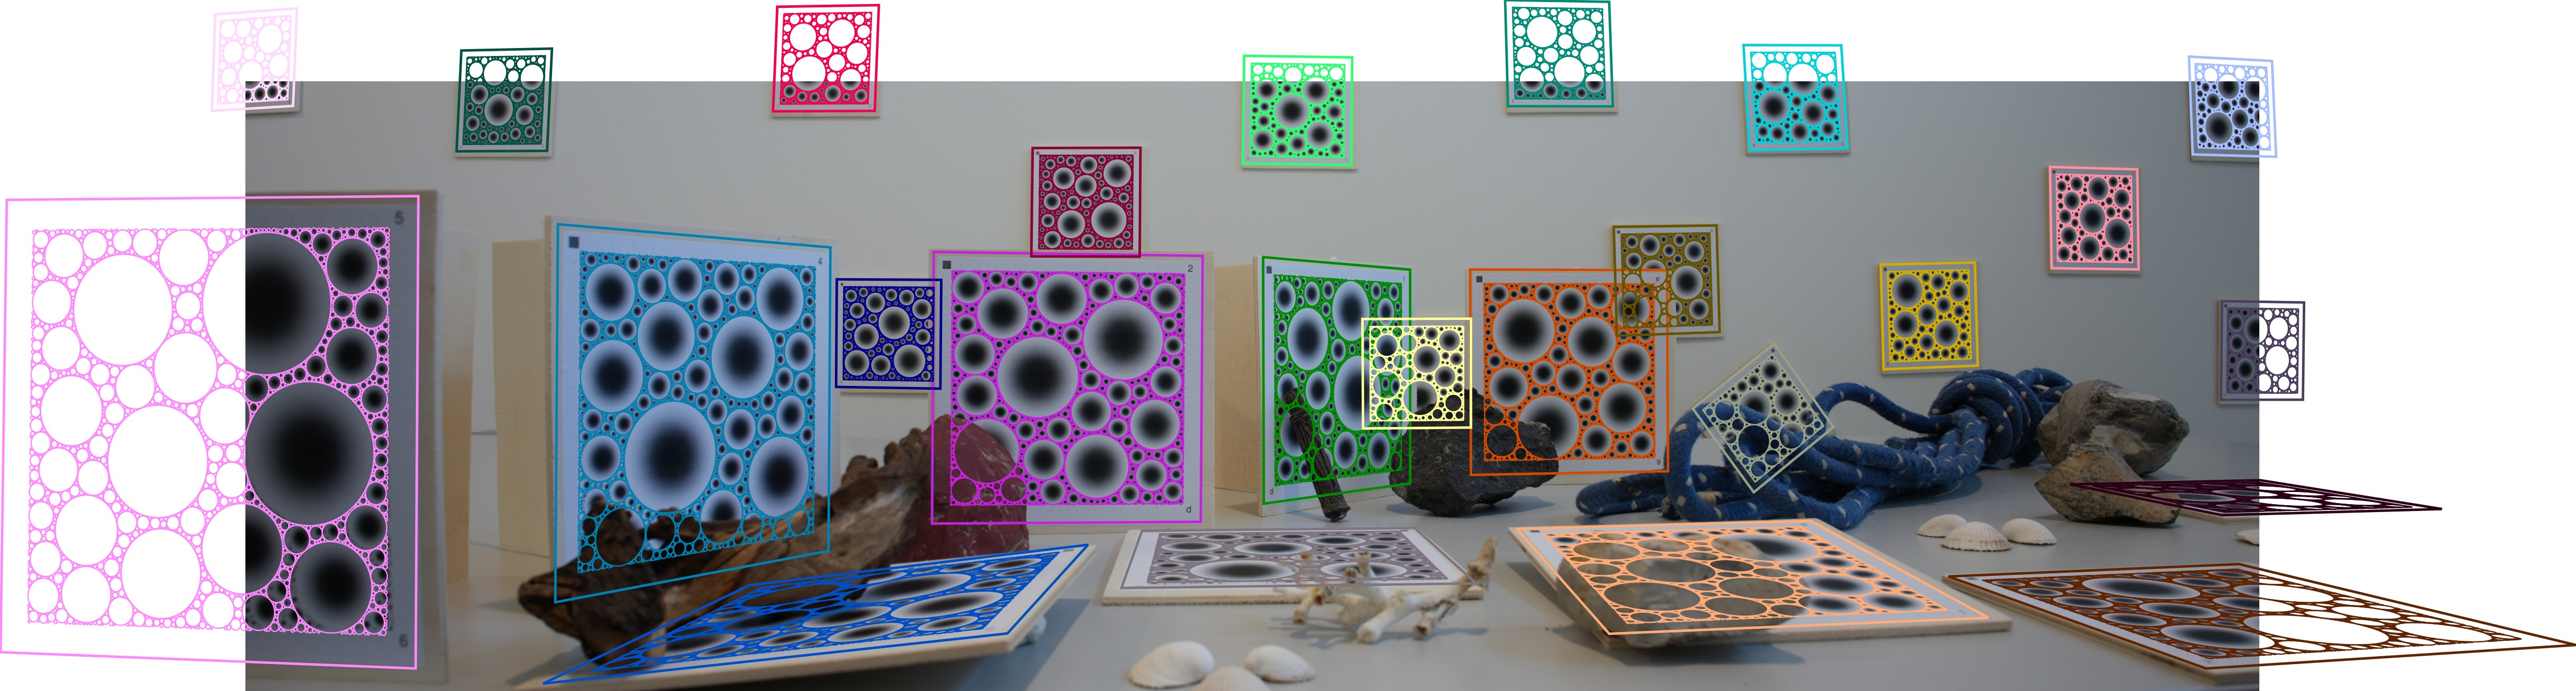
\includegraphics[width=\linewidth]{images/intro_overlay.jpg}
    \end{center}

    \textbf{fiducial marker system} that is
    \begin{itemize}[nosep]
        \item intrinsically multiscale
        \item accurate through coverage density
        \item robust against occlusion
    \end{itemize}
}

\block{Why Blobs?}{
    \begin{minipage}{0.48\linewidth}
        \centering
        {maximises SIFT response}\\[\subcaptiongap]
        \overlaid[width=\linewidth]{images/asift_detections/asift_original_photo.jpg}{images/asift_detections/asift_original.pdf}
    \end{minipage}\hfill%
    \begin{minipage}{0.48\linewidth}
        \centering
        {robust to defocus}\\[\subcaptiongap]
        \overlaid[width=\linewidth]{images/asift_detections/asift_blurred_photo.jpg}{images/asift_detections/asift_blurred.pdf}
    \end{minipage}
}

% one panel is \pipepanel wide (3:4); panels sit \pipegap = 0.047 panels apart
% in both rows, so (d) -- two panels and the gap between them -- is exactly
% 2.047 panels wide, at a panel's height, and its edges line up with (a)/(b)
\newlength{\pipepanel}
\newlength{\pipegap}
\block{Pipeline}{
	\centering
	\setlength{\pipepanel}{0.32\linewidth}%
	\setlength{\pipegap}{0.047\pipepanel}%
	\begin{minipage}{\pipepanel}
		\centering
		{(a) detect}\\[\subcaptiongap]
		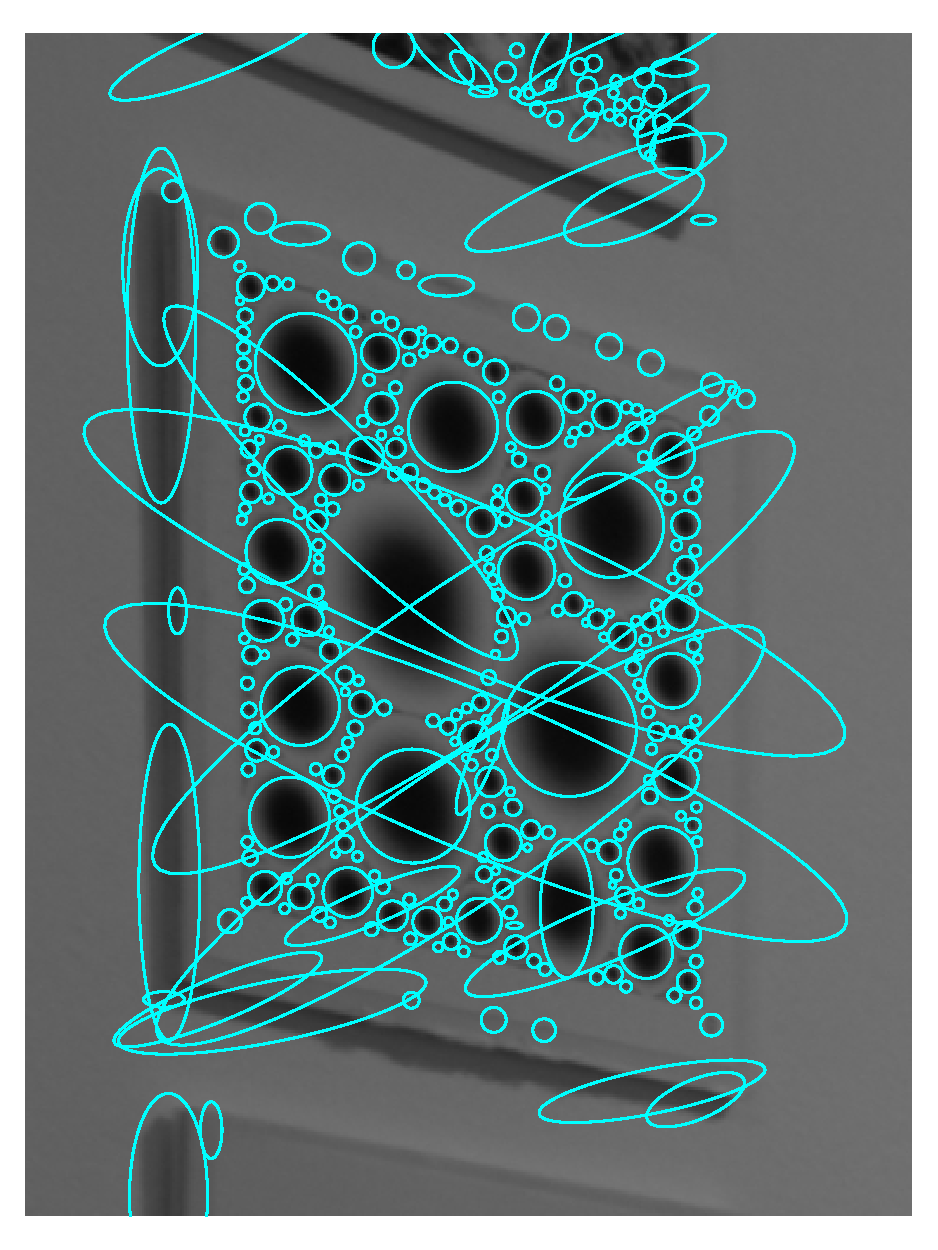
\includegraphics[width=\linewidth]{images/bb_pipe_detect.pdf}
	\end{minipage}\hspace{\pipegap}%
	\begin{minipage}{\pipepanel}
		\centering
		{(b) adapt}\\[\subcaptiongap]
		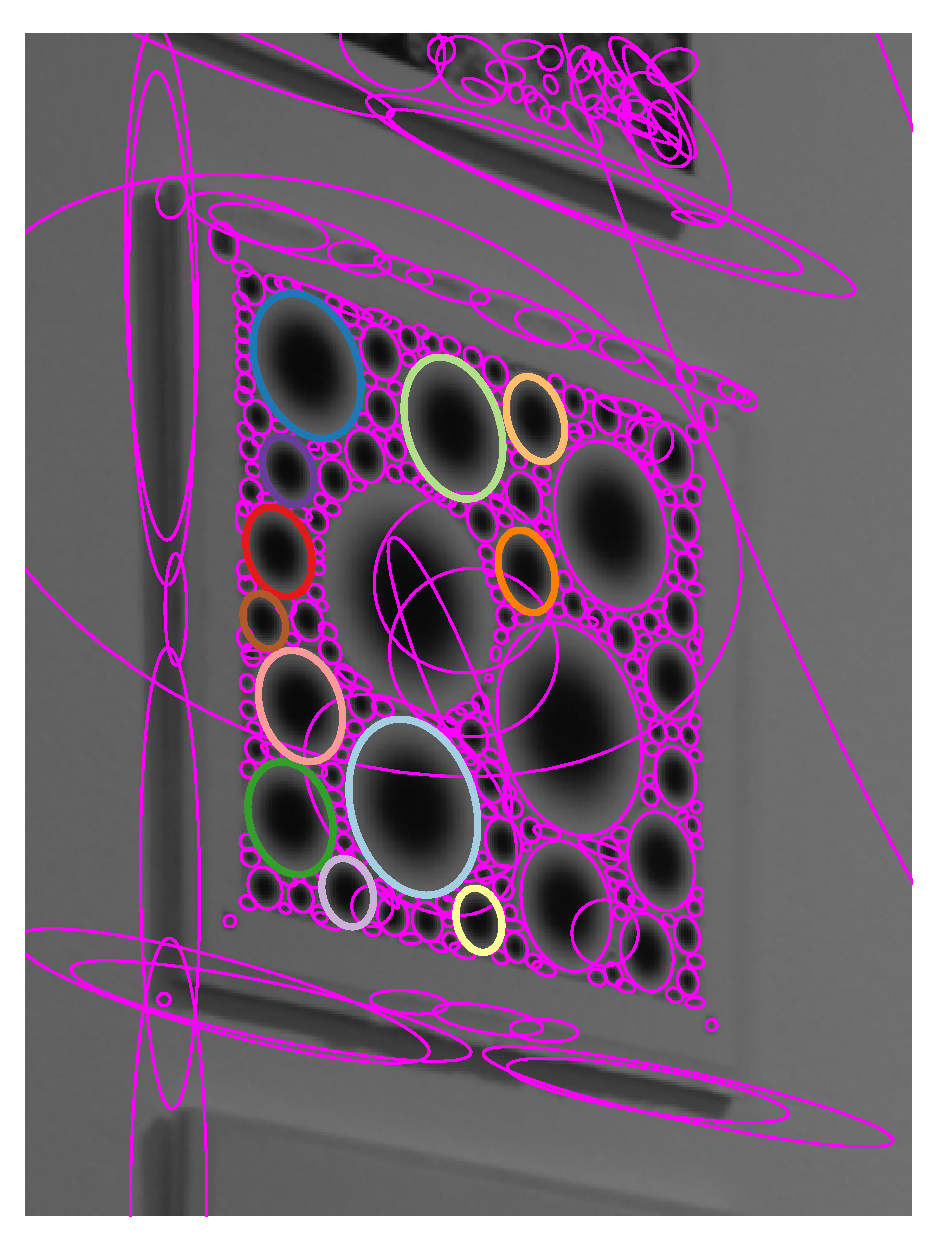
\includegraphics[width=\linewidth]{images/bb_pipe_adapt.pdf}
	\end{minipage}\hspace{\pipegap}%
	\begin{minipage}{\pipepanel}
		\centering
		{(c) canonicalize}\\[\subcaptiongap]
		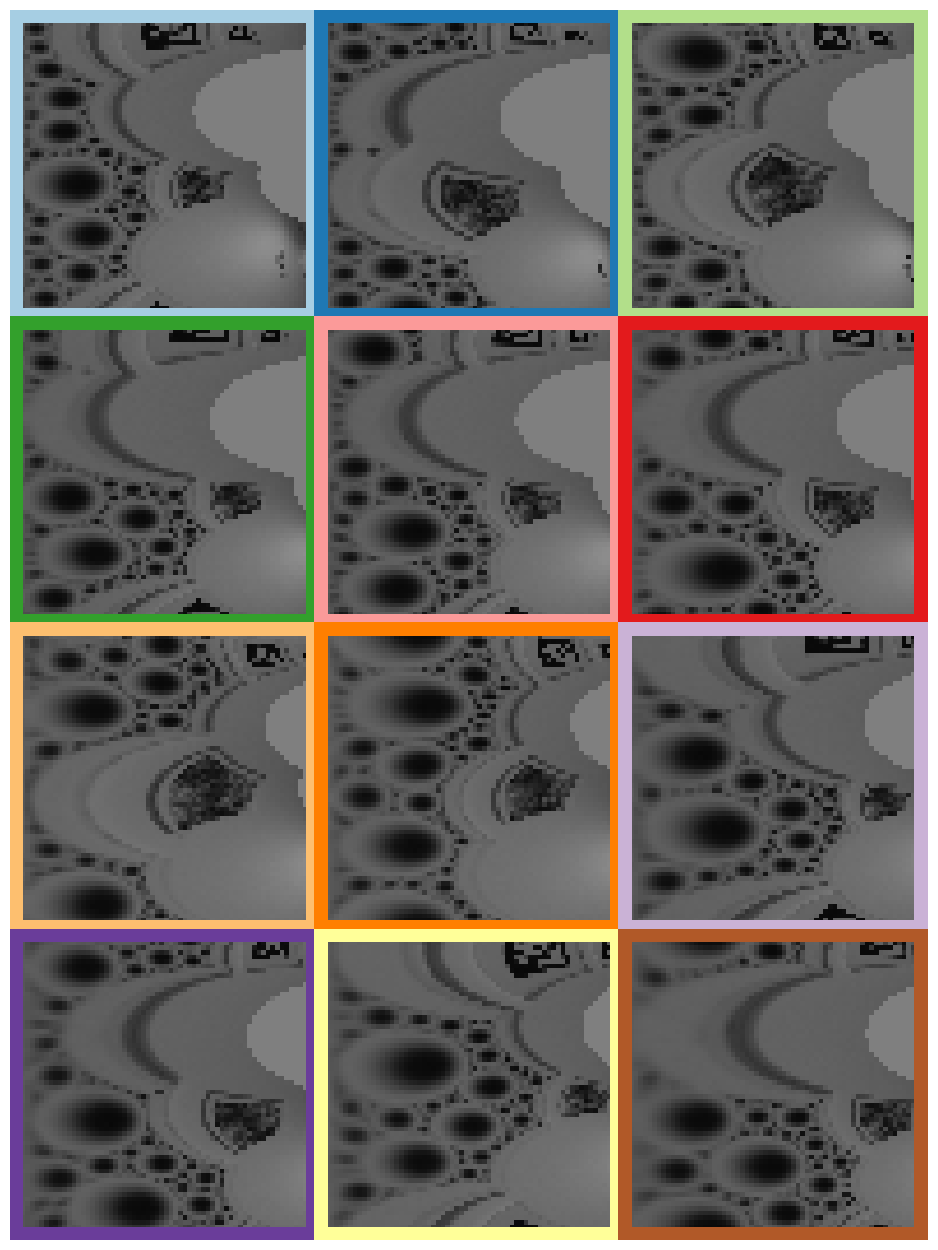
\includegraphics[width=\linewidth]{images/bb_pipe_logpolar.pdf}
	\end{minipage}\\[2\subcaptiongap]
	\begin{minipage}{2.047\pipepanel}
		\centering
		{(d) match}\\[\subcaptiongap]
		\resizebox{\linewidth}{\dimexpr 4\pipepanel/3\relax}{% bb_pipe_match: written by bmvc2026/scripts/make_pipeline_panels.jl; do not edit.
% The match panel as layers on a 921 x 600 pt page: the board's own PDF, the photo
% crop and the csponds (a transparent page). Use: \resizebox{<w>}{<h>}{% bb_pipe_match: written by bmvc2026/scripts/make_pipeline_panels.jl; do not edit.
% The match panel as layers on a 921 x 600 pt page: the board's own PDF, the photo
% crop and the csponds (a transparent page). Use: \resizebox{<w>}{<h>}{% bb_pipe_match: written by bmvc2026/scripts/make_pipeline_panels.jl; do not edit.
% The match panel as layers on a 921 x 600 pt page: the board's own PDF, the photo
% crop and the csponds (a transparent page). Use: \resizebox{<w>}{<h>}{\input{images/bb_pipe_match}}
{\setlength{\unitlength}{1pt}%
\begin{picture}(921,600)%
\put(12.0,87.2435){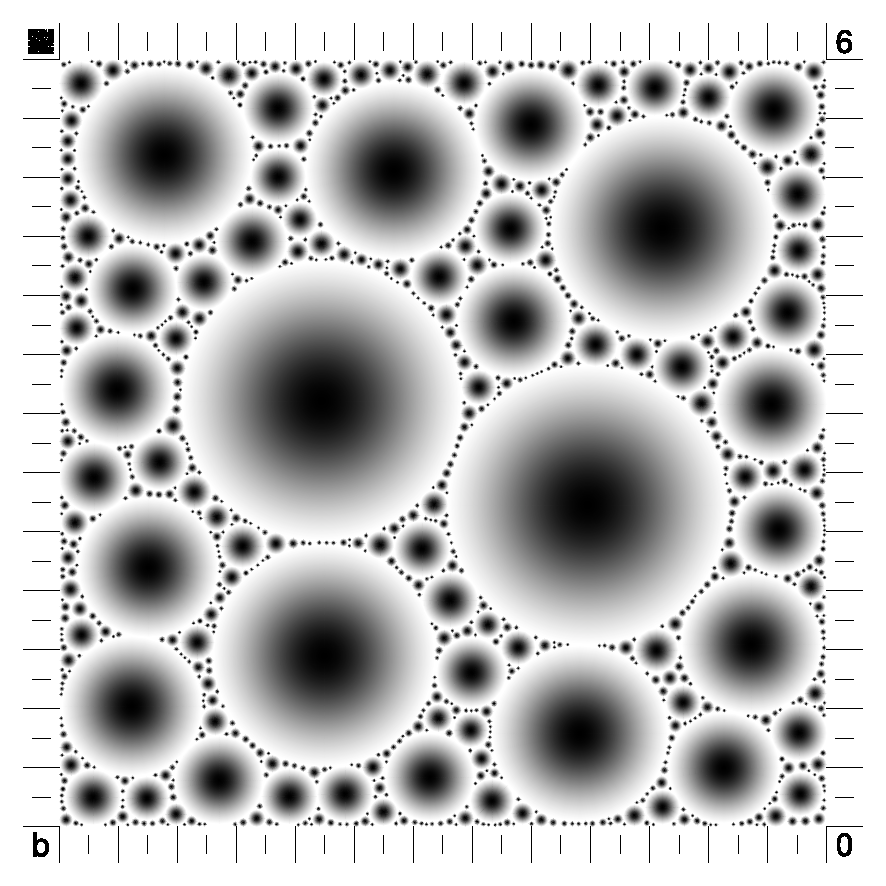
\includegraphics[width=425.5365pt,height=425.5365pt]{images/bb_pipe_match_board.pdf}}%
\put(483.0,16.0){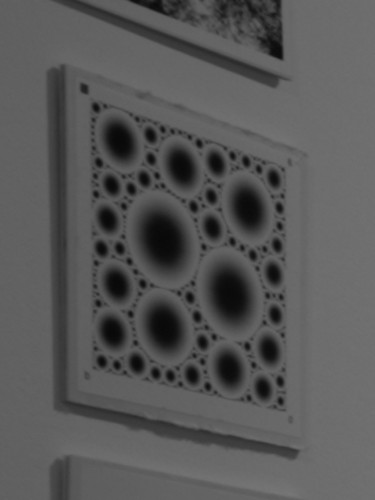
\includegraphics[width=426.0pt,height=568.0pt]{images/bb_pipe_match_photo.jpg}}%
\put(0,0){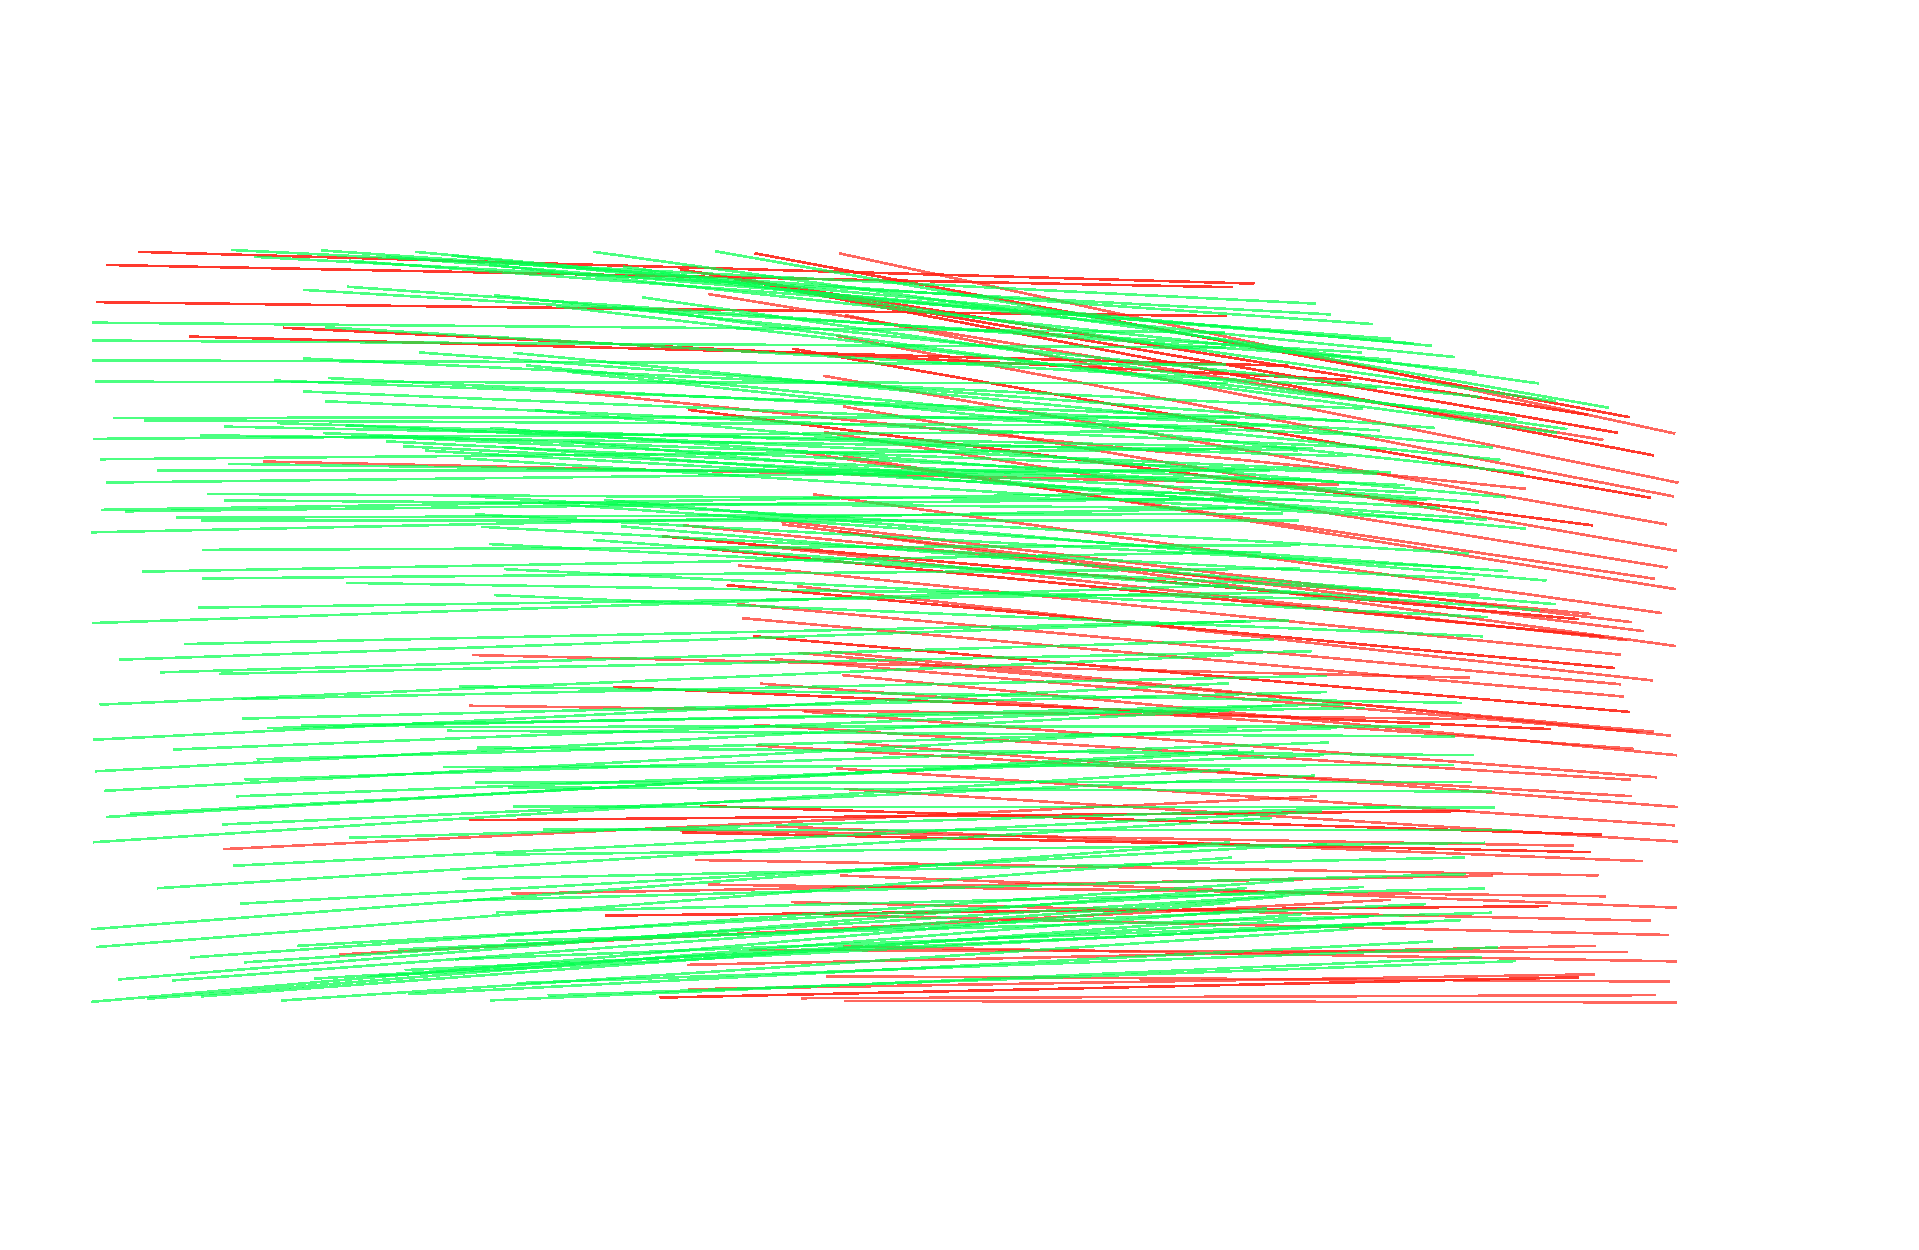
\includegraphics[width=921pt,height=600pt]{images/bb_pipe_match.pdf}}%
\end{picture}}%
}
{\setlength{\unitlength}{1pt}%
\begin{picture}(921,600)%
\put(12.0,87.2435){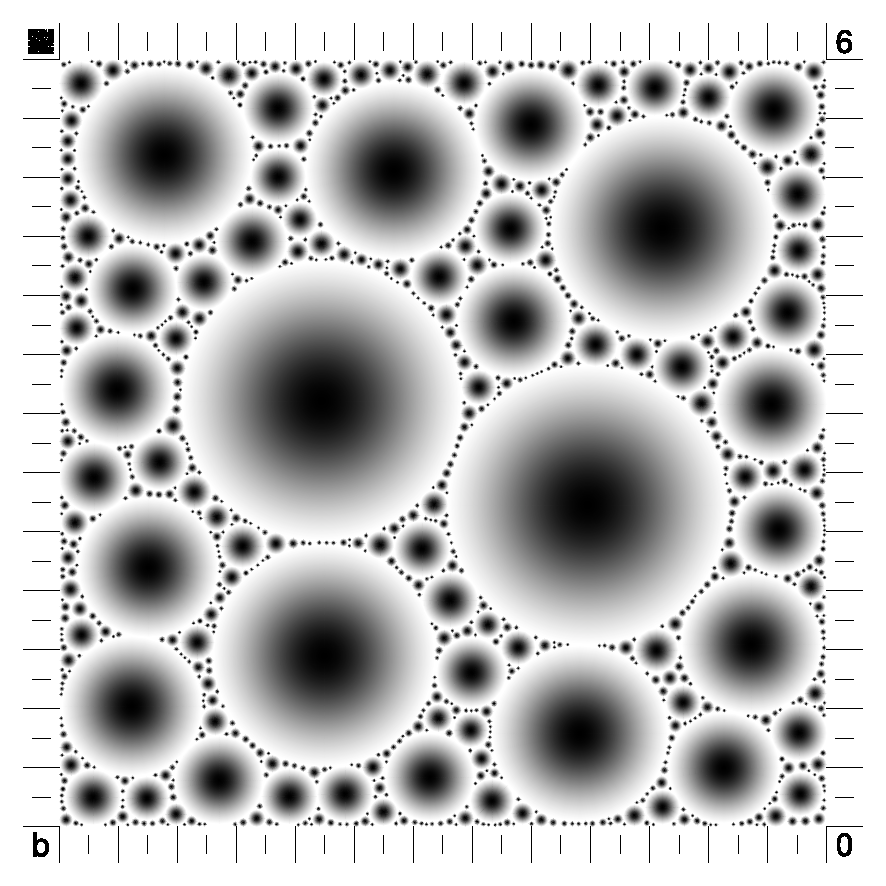
\includegraphics[width=425.5365pt,height=425.5365pt]{images/bb_pipe_match_board.pdf}}%
\put(483.0,16.0){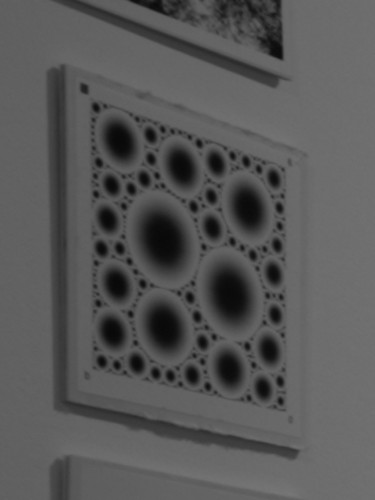
\includegraphics[width=426.0pt,height=568.0pt]{images/bb_pipe_match_photo.jpg}}%
\put(0,0){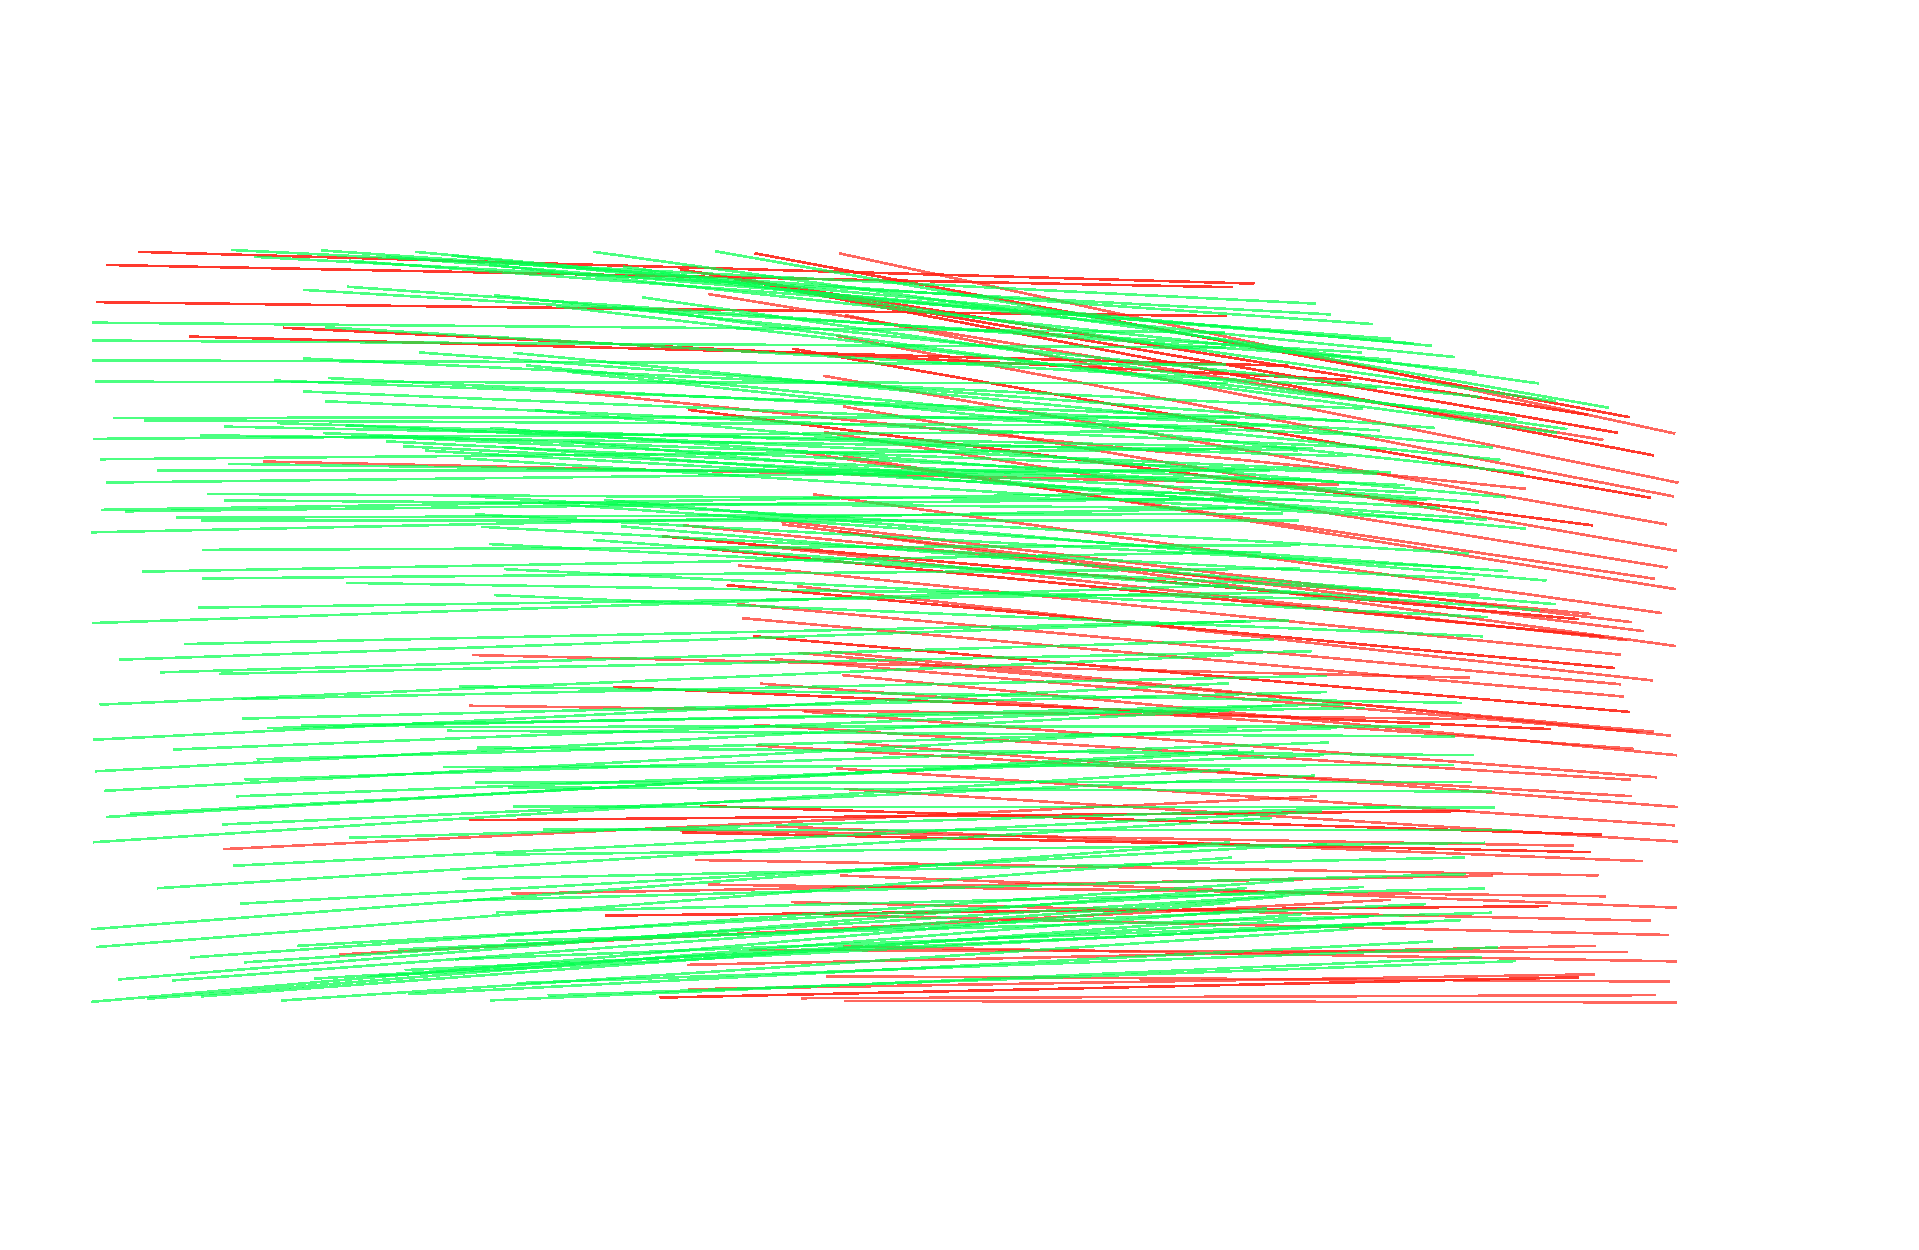
\includegraphics[width=921pt,height=600pt]{images/bb_pipe_match.pdf}}%
\end{picture}}%
}
{\setlength{\unitlength}{1pt}%
\begin{picture}(921,600)%
\put(12.0,87.2435){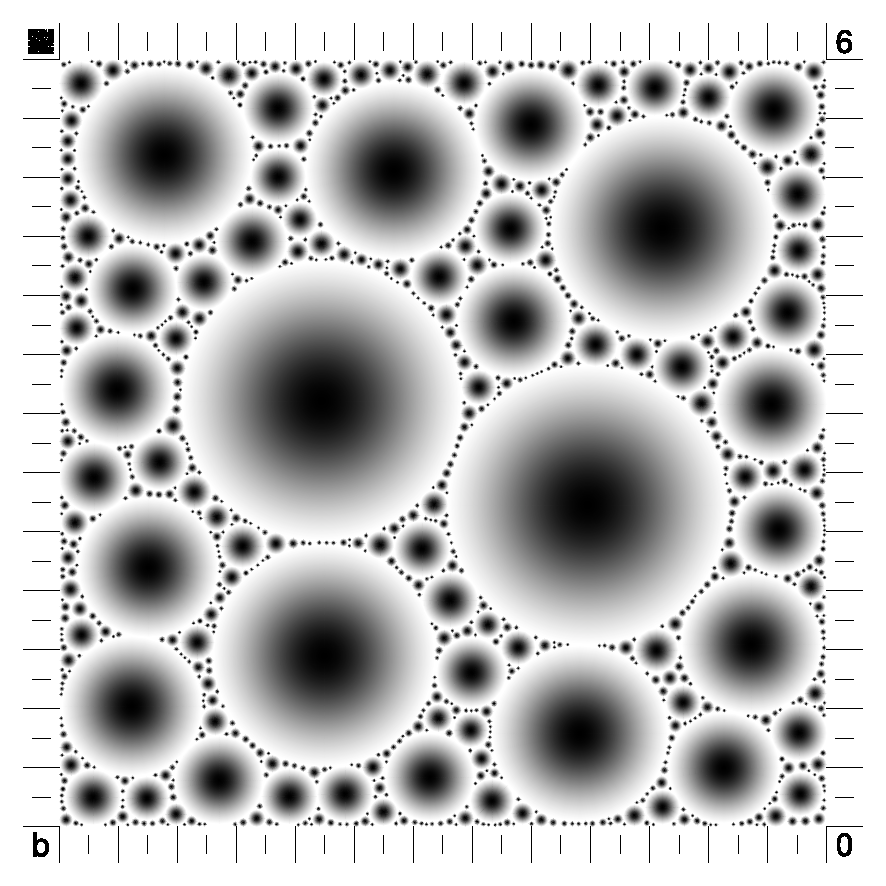
\includegraphics[width=425.5365pt,height=425.5365pt]{images/bb_pipe_match_board.pdf}}%
\put(483.0,16.0){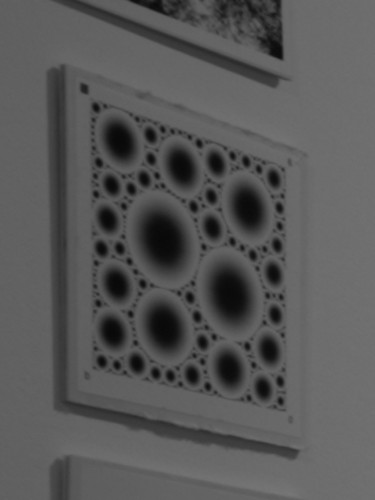
\includegraphics[width=426.0pt,height=568.0pt]{images/bb_pipe_match_photo.jpg}}%
\put(0,0){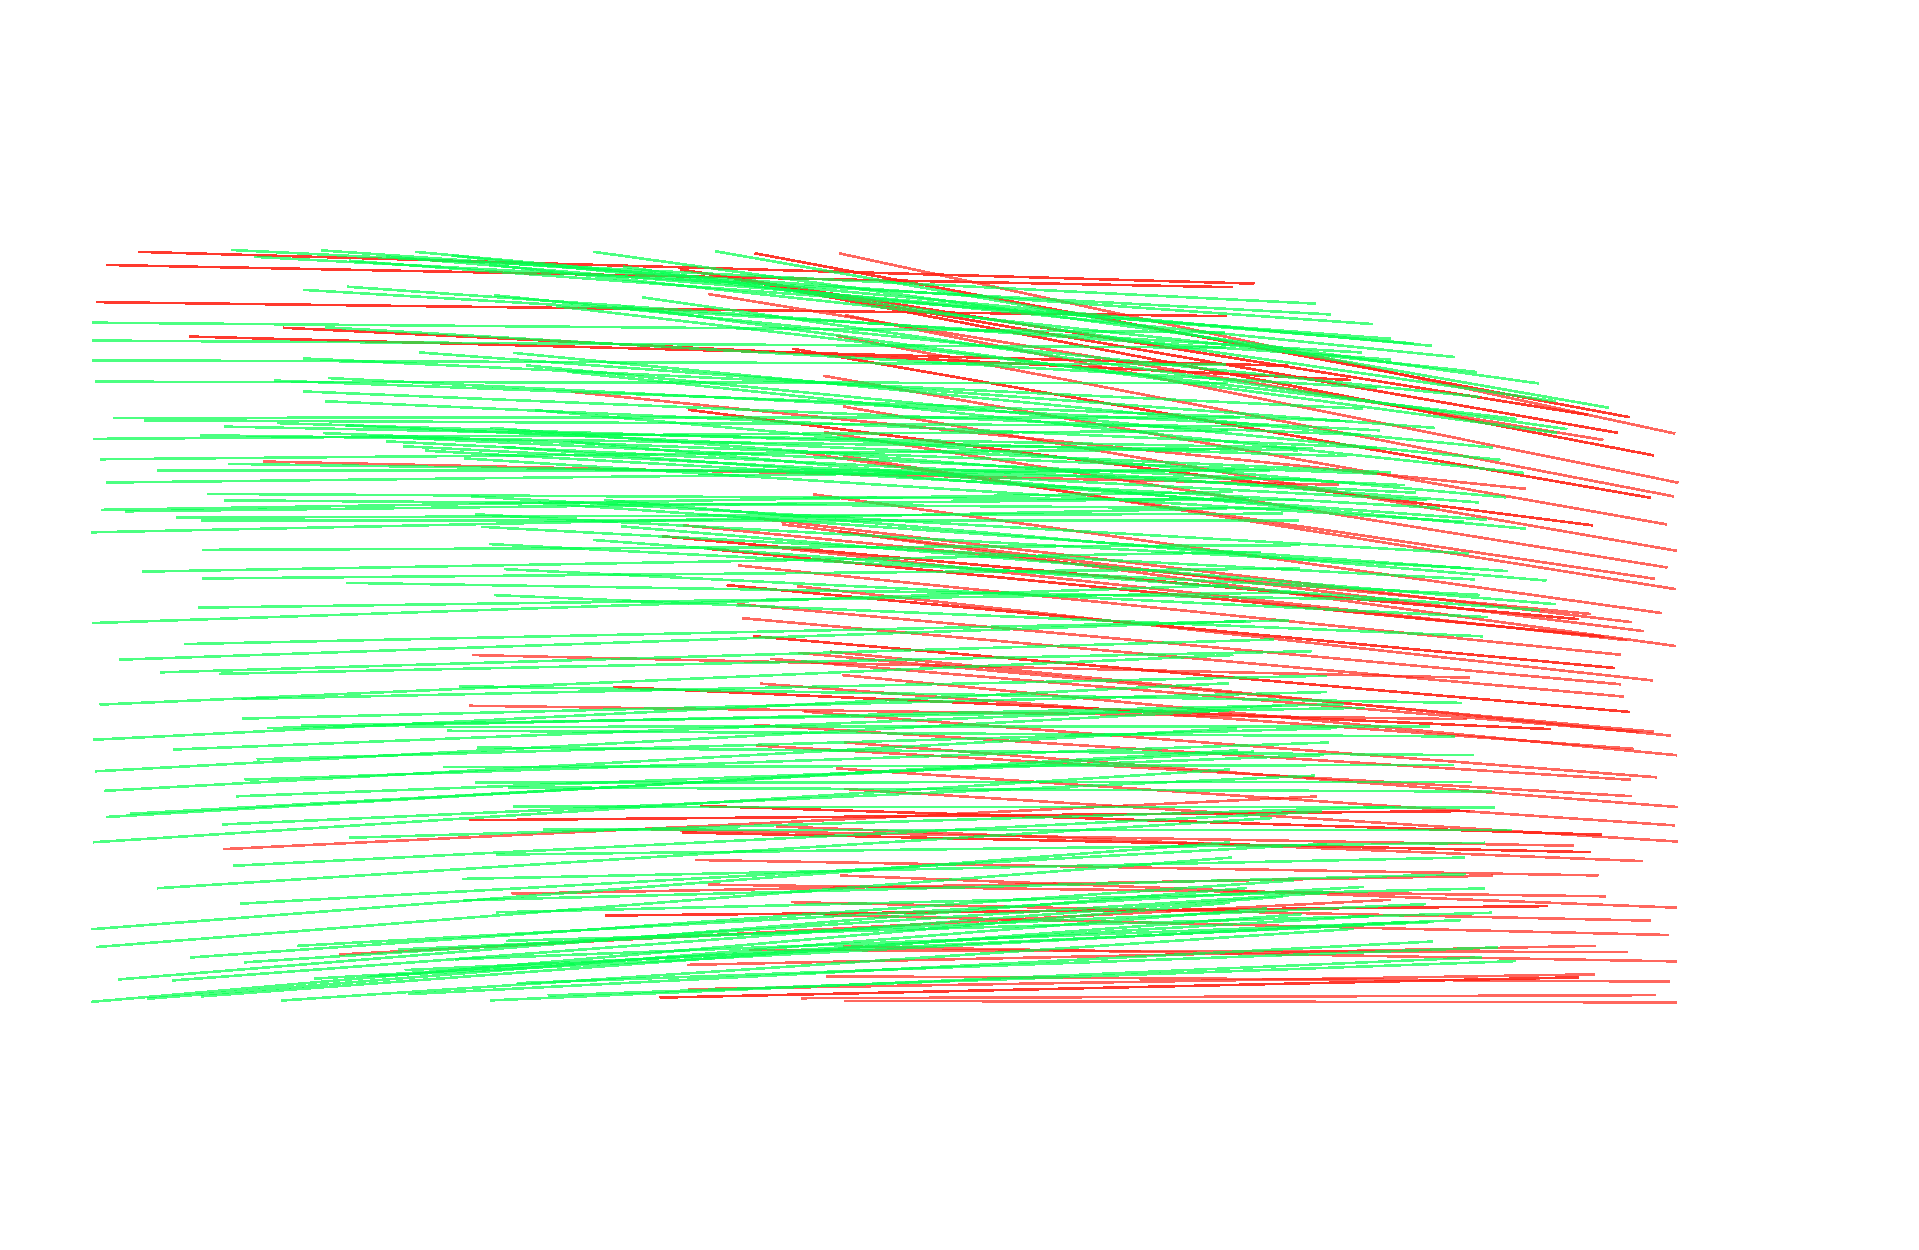
\includegraphics[width=921pt,height=600pt]{images/bb_pipe_match.pdf}}%
\end{picture}}%
}
	\end{minipage}\hspace{\pipegap}%
	\begin{minipage}{\pipepanel}
		\centering
		{(e) estimate pose}\\[\subcaptiongap]
		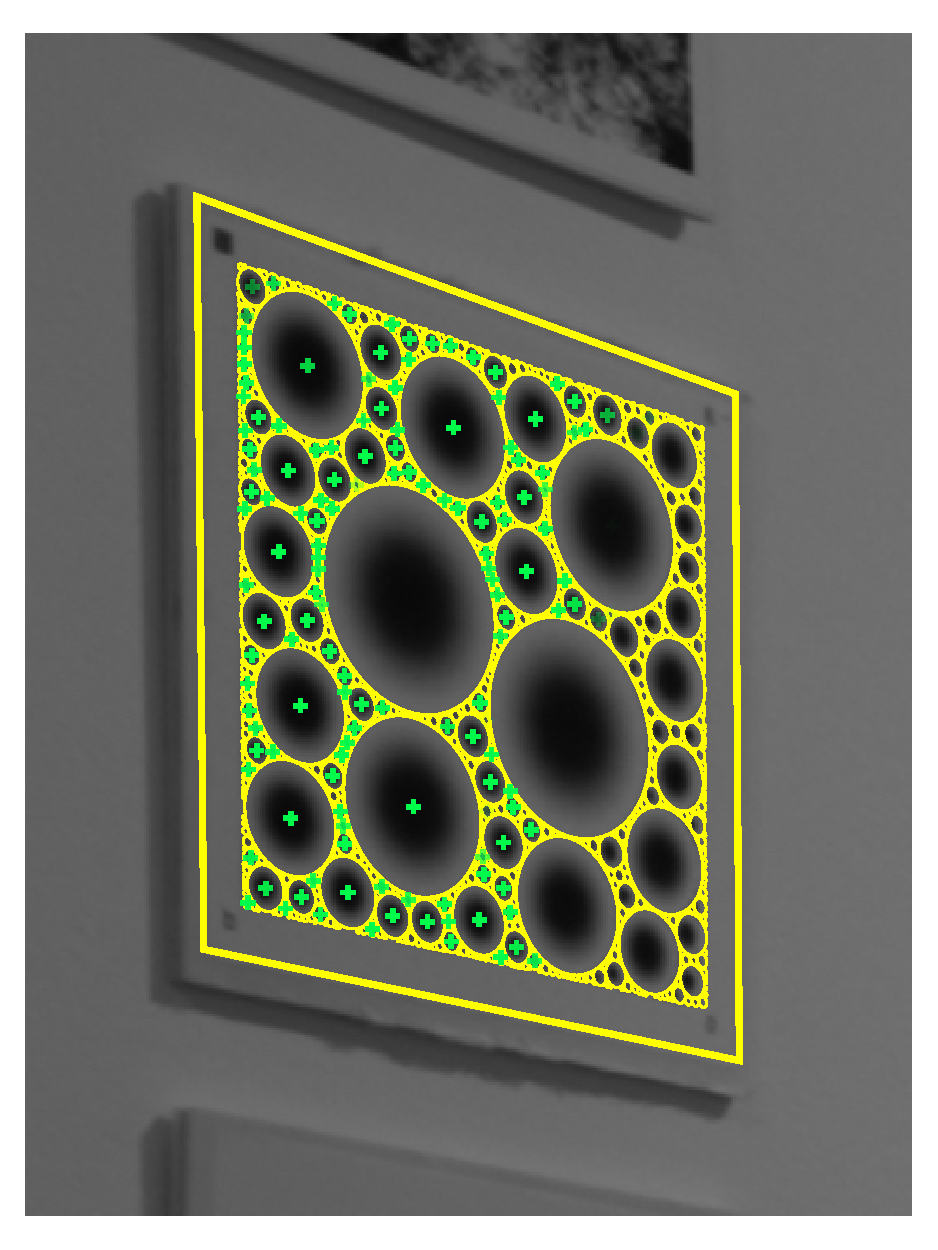
\includegraphics[width=\linewidth]{images/bb_pipe_register.pdf}
	\end{minipage}
}

\block{Experimental Setup}{
	\begin{description}[nosep]
		\item[setup:] 30 boards at different sizes observed from different distances and view angles
		\item[baselines:] AprilTag~3 and OpenCV's ArUco detector
		\item[ground truth:] motion capture
	\end{description}
	\begin{center}
		\begin{minipage}{0.32\linewidth}
			\centering
			{\small BlobBoards}\\[2pt]
			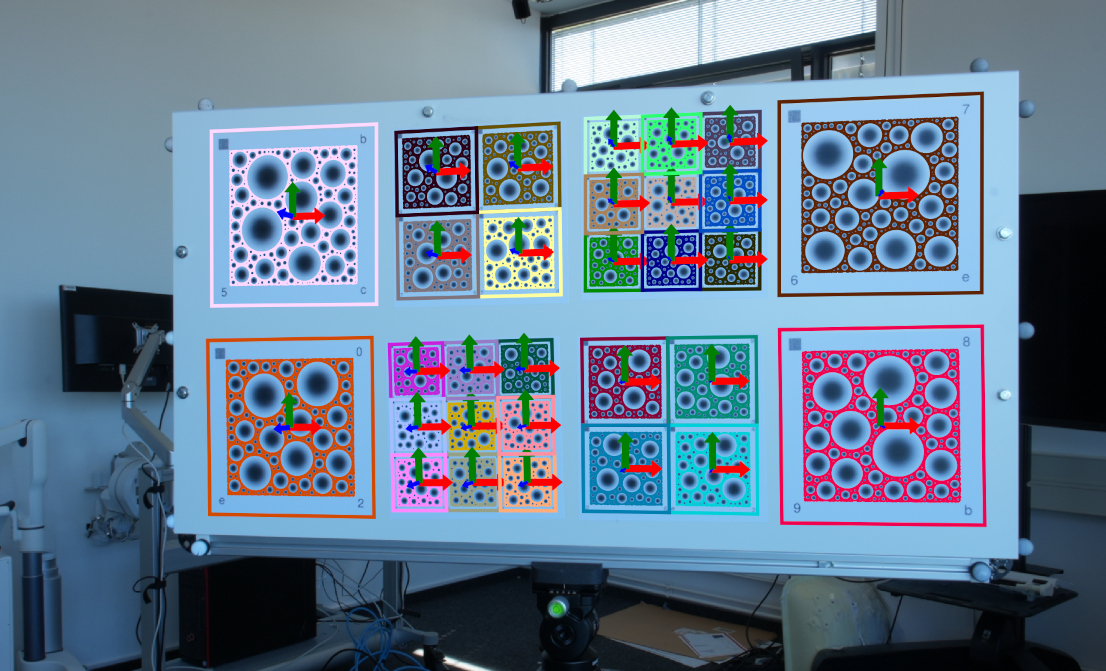
\includegraphics[width=\linewidth]{images/experiment/bb/DSC04530_val.jpg}
		\end{minipage}\hfill
		\begin{minipage}{0.32\linewidth}
			\centering
			{\small AprilTag}\\[2pt]
			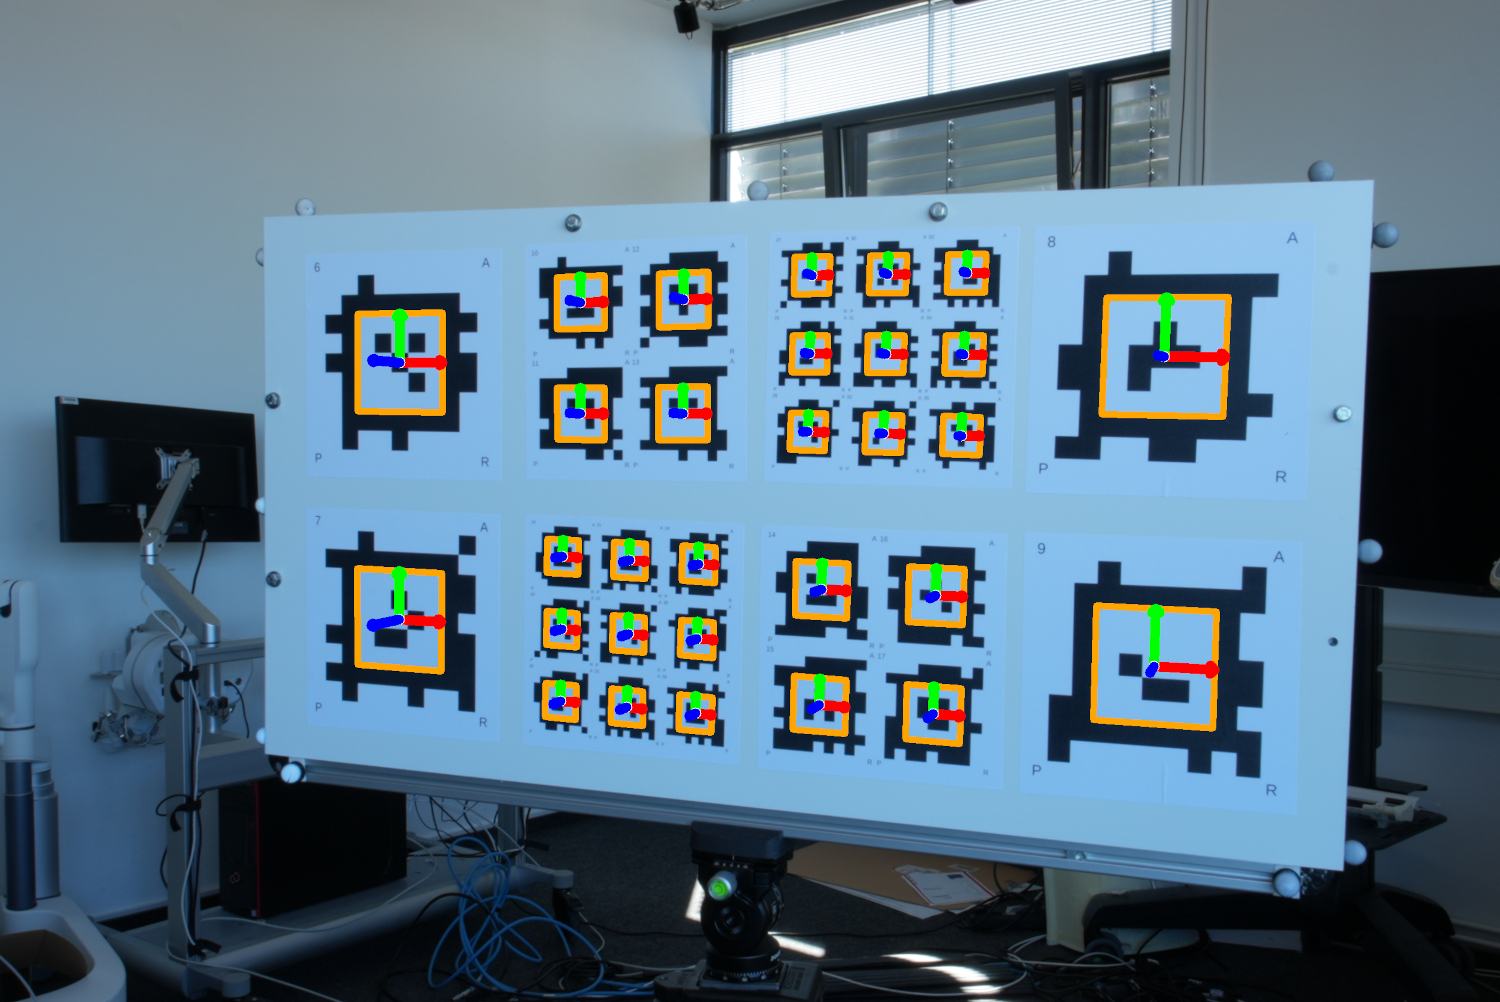
\includegraphics[width=\linewidth]{images/experiment/apr/DSC04433_val.jpg}
		\end{minipage}\hfill
		\begin{minipage}{0.32\linewidth}
			\centering
			{\small ArUco}\\[2pt]
			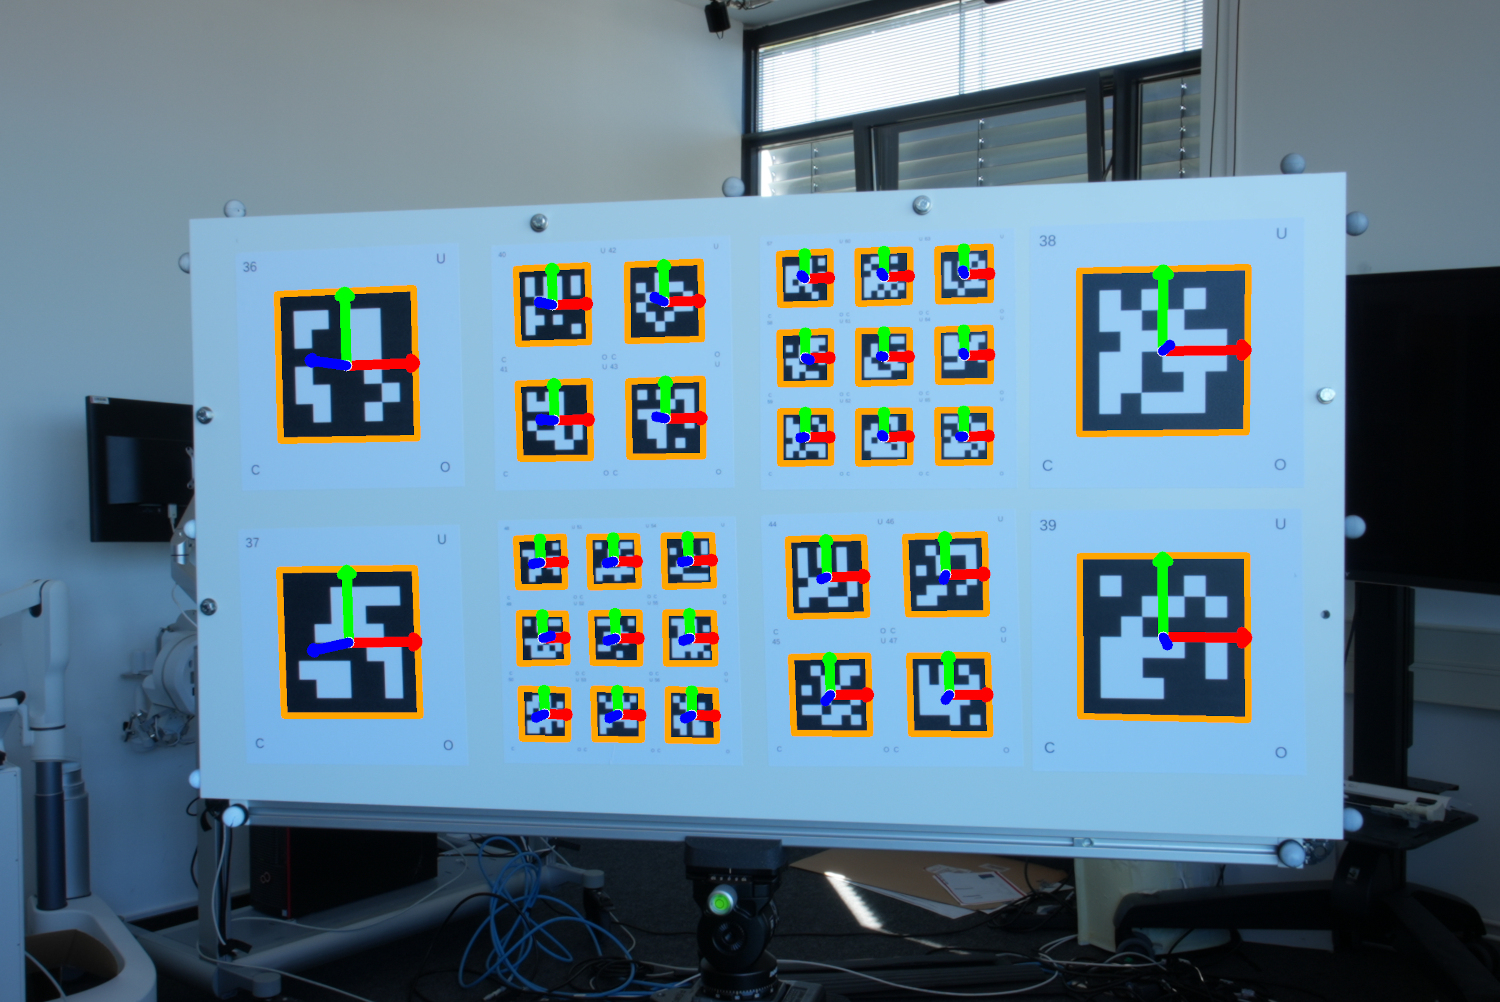
\includegraphics[width=\linewidth]{images/experiment/aru/DSC04343_val.jpg}
		\end{minipage}
	\end{center}
}

\column{0.5}

\block{Results}{
	\begin{center}
		\begin{minipage}{\linewidth}
			\begin{centering}
				\figheading{probability of detection and translation error}
				\resizebox{0.95\linewidth}{!}{%
					\paperfontsettings
					% error_floorplan_ab.tex — generated by error_distributions.jl (rows (a) and (b): no per-station rotation row (not resolvable by the hand-eye ground truth)); do not edit by hand
% class-agnostic: manual (a)/(b)/(c) caption lines, NO subcaption
% (bmvc2k's caption machinery mis-numbers subcaption subfigures)
% requires: \usepackage{graphicx,pgfplots} \pgfplotsset{compat=1.18}
\providecommand{\fpscale}{1}\renewcommand{\fpscale}{0.42}   % fan geometry scale (fonts unaffected)
\setlength{\tabcolsep}{3pt}
\centering
\begin{tabular}{@{}ccc l@{}}
\textbf{BlobBoards} & \textbf{AprilTag} & \textbf{ArUco} & \\[2pt]
% floorplan fan: BlobBoards / det — generated by error_distributions.jl; do not edit by hand
\providecommand{\fpscale}{1}
\begin{tikzpicture}[x=\fpscale cm, y=\fpscale cm, baseline=(current bounding box.north)]
  \fill[fill={rgb,1:red,0.0;green,0.408;blue,0.216}, draw=black!30, line width=0.2pt] (95.0:0.7) arc[start angle=95.0, end angle=85.0, radius=0.7] -- (85.0:1.3) arc[start angle=85.0, end angle=95.0, radius=1.3] -- cycle;
  \fill[fill={rgb,1:red,0.0;green,0.408;blue,0.216}, draw=black!30, line width=0.2pt] (105.0:0.7) arc[start angle=105.0, end angle=95.0, radius=0.7] -- (95.0:1.3) arc[start angle=95.0, end angle=105.0, radius=1.3] -- cycle;
  \fill[fill={rgb,1:red,0.0;green,0.408;blue,0.216}, draw=black!30, line width=0.2pt] (115.0:0.7) arc[start angle=115.0, end angle=105.0, radius=0.7] -- (105.0:1.3) arc[start angle=105.0, end angle=115.0, radius=1.3] -- cycle;
  \fill[fill={rgb,1:red,0.0;green,0.408;blue,0.216}, draw=black!30, line width=0.2pt] (125.0:0.7) arc[start angle=125.0, end angle=115.0, radius=0.7] -- (115.0:1.3) arc[start angle=115.0, end angle=125.0, radius=1.3] -- cycle;
  \fill[fill={rgb,1:red,0.0;green,0.408;blue,0.216}, draw=black!30, line width=0.2pt] (135.0:0.7) arc[start angle=135.0, end angle=125.0, radius=0.7] -- (125.0:1.3) arc[start angle=125.0, end angle=135.0, radius=1.3] -- cycle;
  \fill[fill={rgb,1:red,0.0;green,0.408;blue,0.216}, draw=black!30, line width=0.2pt] (145.0:0.7) arc[start angle=145.0, end angle=135.0, radius=0.7] -- (135.0:1.3) arc[start angle=135.0, end angle=145.0, radius=1.3] -- cycle;
  \fill[fill={rgb,1:red,0.0;green,0.408;blue,0.216}, draw=black!30, line width=0.2pt] (155.0:0.7) arc[start angle=155.0, end angle=145.0, radius=0.7] -- (145.0:1.3) arc[start angle=145.0, end angle=155.0, radius=1.3] -- cycle;
  \fill[fill={rgb,1:red,0.0;green,0.408;blue,0.216}, draw=black!30, line width=0.2pt] (165.0:0.7) arc[start angle=165.0, end angle=155.0, radius=0.7] -- (155.0:1.3) arc[start angle=155.0, end angle=165.0, radius=1.3] -- cycle;
  \fill[fill={rgb,1:red,0.9967;green,0.8983;blue,0.579}, draw=black!30, line width=0.2pt] (175.0:0.7) arc[start angle=175.0, end angle=165.0, radius=0.7] -- (165.0:1.3) arc[start angle=165.0, end angle=175.0, radius=1.3] -- cycle;
  \fill[fill={rgb,1:red,0.0;green,0.408;blue,0.216}, draw=black!30, line width=0.2pt] (85.0:0.7) arc[start angle=85.0, end angle=75.0, radius=0.7] -- (75.0:1.3) arc[start angle=75.0, end angle=85.0, radius=1.3] -- cycle;
  \fill[fill={rgb,1:red,0.0;green,0.408;blue,0.216}, draw=black!30, line width=0.2pt] (75.0:0.7) arc[start angle=75.0, end angle=65.0, radius=0.7] -- (65.0:1.3) arc[start angle=65.0, end angle=75.0, radius=1.3] -- cycle;
  \fill[fill={rgb,1:red,0.0;green,0.408;blue,0.216}, draw=black!30, line width=0.2pt] (65.0:0.7) arc[start angle=65.0, end angle=55.0, radius=0.7] -- (55.0:1.3) arc[start angle=55.0, end angle=65.0, radius=1.3] -- cycle;
  \fill[fill={rgb,1:red,0.0;green,0.408;blue,0.216}, draw=black!30, line width=0.2pt] (55.0:0.7) arc[start angle=55.0, end angle=45.0, radius=0.7] -- (45.0:1.3) arc[start angle=45.0, end angle=55.0, radius=1.3] -- cycle;
  \fill[fill={rgb,1:red,0.0;green,0.408;blue,0.216}, draw=black!30, line width=0.2pt] (45.0:0.7) arc[start angle=45.0, end angle=35.0, radius=0.7] -- (35.0:1.3) arc[start angle=35.0, end angle=45.0, radius=1.3] -- cycle;
  \fill[fill={rgb,1:red,0.0;green,0.408;blue,0.216}, draw=black!30, line width=0.2pt] (35.0:0.7) arc[start angle=35.0, end angle=25.0, radius=0.7] -- (25.0:1.3) arc[start angle=25.0, end angle=35.0, radius=1.3] -- cycle;
  \fill[fill={rgb,1:red,0.0;green,0.408;blue,0.216}, draw=black!30, line width=0.2pt] (25.0:0.7) arc[start angle=25.0, end angle=15.0, radius=0.7] -- (15.0:1.3) arc[start angle=15.0, end angle=25.0, radius=1.3] -- cycle;
  \fill[fill={rgb,1:red,0.862;green,0.2278;blue,0.1713}, draw=black!30, line width=0.2pt] (15.0:0.7) arc[start angle=15.0, end angle=5.0, radius=0.7] -- (5.0:1.3) arc[start angle=5.0, end angle=15.0, radius=1.3] -- cycle;
  \fill[fill={rgb,1:red,0.0;green,0.408;blue,0.216}, draw=black!30, line width=0.2pt] (95.0:1.7) arc[start angle=95.0, end angle=85.0, radius=1.7] -- (85.0:2.3) arc[start angle=85.0, end angle=95.0, radius=2.3] -- cycle;
  \fill[fill={rgb,1:red,0.0;green,0.408;blue,0.216}, draw=black!30, line width=0.2pt] (85.0:1.7) arc[start angle=85.0, end angle=75.0, radius=1.7] -- (75.0:2.3) arc[start angle=75.0, end angle=85.0, radius=2.3] -- cycle;
  \fill[fill={rgb,1:red,0.0;green,0.408;blue,0.216}, draw=black!30, line width=0.2pt] (115.0:1.7) arc[start angle=115.0, end angle=105.0, radius=1.7] -- (105.0:2.3) arc[start angle=105.0, end angle=115.0, radius=2.3] -- cycle;
  \fill[fill={rgb,1:red,0.0;green,0.408;blue,0.216}, draw=black!30, line width=0.2pt] (125.0:1.7) arc[start angle=125.0, end angle=115.0, radius=1.7] -- (115.0:2.3) arc[start angle=115.0, end angle=125.0, radius=2.3] -- cycle;
  \fill[fill={rgb,1:red,0.0;green,0.408;blue,0.216}, draw=black!30, line width=0.2pt] (135.0:1.7) arc[start angle=135.0, end angle=125.0, radius=1.7] -- (125.0:2.3) arc[start angle=125.0, end angle=135.0, radius=2.3] -- cycle;
  \fill[fill={rgb,1:red,0.0;green,0.408;blue,0.216}, draw=black!30, line width=0.2pt] (145.0:1.7) arc[start angle=145.0, end angle=135.0, radius=1.7] -- (135.0:2.3) arc[start angle=135.0, end angle=145.0, radius=2.3] -- cycle;
  \fill[fill={rgb,1:red,0.0;green,0.408;blue,0.216}, draw=black!30, line width=0.2pt] (155.0:1.7) arc[start angle=155.0, end angle=145.0, radius=1.7] -- (145.0:2.3) arc[start angle=145.0, end angle=155.0, radius=2.3] -- cycle;
  \fill[fill={rgb,1:red,0.0;green,0.408;blue,0.216}, draw=black!30, line width=0.2pt] (165.0:1.7) arc[start angle=165.0, end angle=155.0, radius=1.7] -- (155.0:2.3) arc[start angle=155.0, end angle=165.0, radius=2.3] -- cycle;
  \fill[fill={rgb,1:red,0.7777;green,0.1253;blue,0.1517}, draw=black!30, line width=0.2pt] (175.0:1.7) arc[start angle=175.0, end angle=165.0, radius=1.7] -- (165.0:2.3) arc[start angle=165.0, end angle=175.0, radius=2.3] -- cycle;
  \fill[fill={rgb,1:red,0.0;green,0.408;blue,0.216}, draw=black!30, line width=0.2pt] (75.0:1.7) arc[start angle=75.0, end angle=65.0, radius=1.7] -- (65.0:2.3) arc[start angle=65.0, end angle=75.0, radius=2.3] -- cycle;
  \fill[fill={rgb,1:red,0.0;green,0.408;blue,0.216}, draw=black!30, line width=0.2pt] (65.0:1.7) arc[start angle=65.0, end angle=55.0, radius=1.7] -- (55.0:2.3) arc[start angle=55.0, end angle=65.0, radius=2.3] -- cycle;
  \fill[fill={rgb,1:red,0.0;green,0.408;blue,0.216}, draw=black!30, line width=0.2pt] (55.0:1.7) arc[start angle=55.0, end angle=45.0, radius=1.7] -- (45.0:2.3) arc[start angle=45.0, end angle=55.0, radius=2.3] -- cycle;
  \fill[fill={rgb,1:red,0.0;green,0.408;blue,0.216}, draw=black!30, line width=0.2pt] (45.0:1.7) arc[start angle=45.0, end angle=35.0, radius=1.7] -- (35.0:2.3) arc[start angle=35.0, end angle=45.0, radius=2.3] -- cycle;
  \fill[fill={rgb,1:red,0.0;green,0.408;blue,0.216}, draw=black!30, line width=0.2pt] (35.0:1.7) arc[start angle=35.0, end angle=25.0, radius=1.7] -- (25.0:2.3) arc[start angle=25.0, end angle=35.0, radius=2.3] -- cycle;
  \fill[fill={rgb,1:red,0.102;green,0.596;blue,0.314}, draw=black!30, line width=0.2pt] (25.0:1.7) arc[start angle=25.0, end angle=15.0, radius=1.7] -- (15.0:2.3) arc[start angle=15.0, end angle=25.0, radius=2.3] -- cycle;
  \fill[fill={rgb,1:red,0.745;green,0.094;blue,0.151}, draw=black!30, line width=0.2pt] (15.0:1.7) arc[start angle=15.0, end angle=5.0, radius=1.7] -- (5.0:2.3) arc[start angle=5.0, end angle=15.0, radius=2.3] -- cycle;
  \fill[fill={rgb,1:red,0.0;green,0.408;blue,0.216}, draw=black!30, line width=0.2pt] (95.0:2.7) arc[start angle=95.0, end angle=85.0, radius=2.7] -- (85.0:3.3) arc[start angle=85.0, end angle=95.0, radius=3.3] -- cycle;
  \fill[fill={rgb,1:red,0.0;green,0.408;blue,0.216}, draw=black!30, line width=0.2pt] (105.0:2.7) arc[start angle=105.0, end angle=95.0, radius=2.7] -- (95.0:3.3) arc[start angle=95.0, end angle=105.0, radius=3.3] -- cycle;
  \fill[fill={rgb,1:red,0.0;green,0.408;blue,0.216}, draw=black!30, line width=0.2pt] (115.0:2.7) arc[start angle=115.0, end angle=105.0, radius=2.7] -- (105.0:3.3) arc[start angle=105.0, end angle=115.0, radius=3.3] -- cycle;
  \fill[fill={rgb,1:red,0.0;green,0.408;blue,0.216}, draw=black!30, line width=0.2pt] (125.0:2.7) arc[start angle=125.0, end angle=115.0, radius=2.7] -- (115.0:3.3) arc[start angle=115.0, end angle=125.0, radius=3.3] -- cycle;
  \fill[fill={rgb,1:red,0.0;green,0.408;blue,0.216}, draw=black!30, line width=0.2pt] (135.0:2.7) arc[start angle=135.0, end angle=125.0, radius=2.7] -- (125.0:3.3) arc[start angle=125.0, end angle=135.0, radius=3.3] -- cycle;
  \fill[fill={rgb,1:red,0.0;green,0.408;blue,0.216}, draw=black!30, line width=0.2pt] (145.0:2.7) arc[start angle=145.0, end angle=135.0, radius=2.7] -- (135.0:3.3) arc[start angle=135.0, end angle=145.0, radius=3.3] -- cycle;
  \fill[fill={rgb,1:red,0.034;green,0.4707;blue,0.2487}, draw=black!30, line width=0.2pt] (155.0:2.7) arc[start angle=155.0, end angle=145.0, radius=2.7] -- (145.0:3.3) arc[start angle=145.0, end angle=155.0, radius=3.3] -- cycle;
  \fill[fill={rgb,1:red,0.9947;green,0.8127;blue,0.49}, draw=black!30, line width=0.2pt] (165.0:2.7) arc[start angle=165.0, end angle=155.0, radius=2.7] -- (155.0:3.3) arc[start angle=155.0, end angle=165.0, radius=3.3] -- cycle;
  \fill[fill={rgb,1:red,0.6797;green,0.0313;blue,0.1497}, draw=black!30, line width=0.2pt] (175.0:2.7) arc[start angle=175.0, end angle=165.0, radius=2.7] -- (165.0:3.3) arc[start angle=165.0, end angle=175.0, radius=3.3] -- cycle;
  \fill[fill={rgb,1:red,0.0;green,0.408;blue,0.216}, draw=black!30, line width=0.2pt] (85.0:2.7) arc[start angle=85.0, end angle=75.0, radius=2.7] -- (75.0:3.3) arc[start angle=75.0, end angle=85.0, radius=3.3] -- cycle;
  \fill[fill={rgb,1:red,0.0;green,0.408;blue,0.216}, draw=black!30, line width=0.2pt] (75.0:2.7) arc[start angle=75.0, end angle=65.0, radius=2.7] -- (65.0:3.3) arc[start angle=65.0, end angle=75.0, radius=3.3] -- cycle;
  \fill[fill={rgb,1:red,0.0;green,0.408;blue,0.216}, draw=black!30, line width=0.2pt] (65.0:2.7) arc[start angle=65.0, end angle=55.0, radius=2.7] -- (55.0:3.3) arc[start angle=55.0, end angle=65.0, radius=3.3] -- cycle;
  \fill[fill={rgb,1:red,0.0;green,0.408;blue,0.216}, draw=black!30, line width=0.2pt] (55.0:2.7) arc[start angle=55.0, end angle=45.0, radius=2.7] -- (45.0:3.3) arc[start angle=45.0, end angle=55.0, radius=3.3] -- cycle;
  \fill[fill={rgb,1:red,0.0;green,0.408;blue,0.216}, draw=black!30, line width=0.2pt] (45.0:2.7) arc[start angle=45.0, end angle=35.0, radius=2.7] -- (35.0:3.3) arc[start angle=35.0, end angle=45.0, radius=3.3] -- cycle;
  \fill[fill={rgb,1:red,0.3007;green,0.6927;blue,0.3633}, draw=black!30, line width=0.2pt] (35.0:2.7) arc[start angle=35.0, end angle=25.0, radius=2.7] -- (25.0:3.3) arc[start angle=25.0, end angle=35.0, radius=3.3] -- cycle;
  \fill[fill={rgb,1:red,0.992;green,0.682;blue,0.38}, draw=black!30, line width=0.2pt] (25.0:2.7) arc[start angle=25.0, end angle=15.0, radius=2.7] -- (15.0:3.3) arc[start angle=15.0, end angle=25.0, radius=3.3] -- cycle;
  \fill[fill=gray!30, draw=black!30, line width=0.2pt] (15.0:2.7) arc[start angle=15.0, end angle=5.0, radius=2.7] -- (5.0:3.3) arc[start angle=5.0, end angle=15.0, radius=3.3] -- cycle;
  \fill[fill=gray!30, draw=black!30, line width=0.2pt] (105.0:1.7) arc[start angle=105.0, end angle=95.0, radius=1.7] -- (95.0:2.3) arc[start angle=95.0, end angle=105.0, radius=2.3] -- cycle;
  \fill[black] (-0.09, -0.09) rectangle (0.09, 0.09);
  \node[font=\scriptsize\bfseries, text=black!60] at (1, -0.22) {1\,m};
  \node[font=\scriptsize\bfseries, text=black!60] at (2, -0.22) {2\,m};
  \node[font=\scriptsize\bfseries, text=black!60] at (3, -0.22) {3\,m};
\end{tikzpicture}
 & % floorplan fan: AprilTag / det — generated by error_distributions.jl; do not edit by hand
\providecommand{\fpscale}{1}
\begin{tikzpicture}[x=\fpscale cm, y=\fpscale cm, baseline=(current bounding box.north)]
  \fill[fill={rgb,1:red,0.0;green,0.408;blue,0.216}, draw=black!30, line width=0.2pt] (95.0:0.7) arc[start angle=95.0, end angle=85.0, radius=0.7] -- (85.0:1.3) arc[start angle=85.0, end angle=95.0, radius=1.3] -- cycle;
  \fill[fill={rgb,1:red,0.0;green,0.408;blue,0.216}, draw=black!30, line width=0.2pt] (105.0:0.7) arc[start angle=105.0, end angle=95.0, radius=0.7] -- (95.0:1.3) arc[start angle=95.0, end angle=105.0, radius=1.3] -- cycle;
  \fill[fill={rgb,1:red,0.0;green,0.408;blue,0.216}, draw=black!30, line width=0.2pt] (115.0:0.7) arc[start angle=115.0, end angle=105.0, radius=0.7] -- (105.0:1.3) arc[start angle=105.0, end angle=115.0, radius=1.3] -- cycle;
  \fill[fill={rgb,1:red,0.0;green,0.408;blue,0.216}, draw=black!30, line width=0.2pt] (125.0:0.7) arc[start angle=125.0, end angle=115.0, radius=0.7] -- (115.0:1.3) arc[start angle=115.0, end angle=125.0, radius=1.3] -- cycle;
  \fill[fill={rgb,1:red,0.0;green,0.408;blue,0.216}, draw=black!30, line width=0.2pt] (135.0:0.7) arc[start angle=135.0, end angle=125.0, radius=0.7] -- (125.0:1.3) arc[start angle=125.0, end angle=135.0, radius=1.3] -- cycle;
  \fill[fill={rgb,1:red,0.0;green,0.408;blue,0.216}, draw=black!30, line width=0.2pt] (145.0:0.7) arc[start angle=145.0, end angle=135.0, radius=0.7] -- (135.0:1.3) arc[start angle=135.0, end angle=145.0, radius=1.3] -- cycle;
  \fill[fill={rgb,1:red,0.0;green,0.408;blue,0.216}, draw=black!30, line width=0.2pt] (155.0:0.7) arc[start angle=155.0, end angle=145.0, radius=0.7] -- (145.0:1.3) arc[start angle=145.0, end angle=155.0, radius=1.3] -- cycle;
  \fill[fill={rgb,1:red,0.068;green,0.5333;blue,0.2813}, draw=black!30, line width=0.2pt] (165.0:0.7) arc[start angle=165.0, end angle=155.0, radius=0.7] -- (155.0:1.3) arc[start angle=155.0, end angle=165.0, radius=1.3] -- cycle;
  \fill[fill={rgb,1:red,0.745;green,0.094;blue,0.151}, draw=black!30, line width=0.2pt] (175.0:0.7) arc[start angle=175.0, end angle=165.0, radius=0.7] -- (165.0:1.3) arc[start angle=165.0, end angle=175.0, radius=1.3] -- cycle;
  \fill[fill={rgb,1:red,0.0;green,0.408;blue,0.216}, draw=black!30, line width=0.2pt] (85.0:0.7) arc[start angle=85.0, end angle=75.0, radius=0.7] -- (75.0:1.3) arc[start angle=75.0, end angle=85.0, radius=1.3] -- cycle;
  \fill[fill={rgb,1:red,0.0;green,0.408;blue,0.216}, draw=black!30, line width=0.2pt] (75.0:0.7) arc[start angle=75.0, end angle=65.0, radius=0.7] -- (65.0:1.3) arc[start angle=65.0, end angle=75.0, radius=1.3] -- cycle;
  \fill[fill={rgb,1:red,0.0;green,0.408;blue,0.216}, draw=black!30, line width=0.2pt] (65.0:0.7) arc[start angle=65.0, end angle=55.0, radius=0.7] -- (55.0:1.3) arc[start angle=55.0, end angle=65.0, radius=1.3] -- cycle;
  \fill[fill={rgb,1:red,0.0;green,0.408;blue,0.216}, draw=black!30, line width=0.2pt] (55.0:0.7) arc[start angle=55.0, end angle=45.0, radius=0.7] -- (45.0:1.3) arc[start angle=45.0, end angle=55.0, radius=1.3] -- cycle;
  \fill[fill={rgb,1:red,0.0;green,0.408;blue,0.216}, draw=black!30, line width=0.2pt] (45.0:0.7) arc[start angle=45.0, end angle=35.0, radius=0.7] -- (35.0:1.3) arc[start angle=35.0, end angle=45.0, radius=1.3] -- cycle;
  \fill[fill={rgb,1:red,0.0;green,0.408;blue,0.216}, draw=black!30, line width=0.2pt] (35.0:0.7) arc[start angle=35.0, end angle=25.0, radius=0.7] -- (25.0:1.3) arc[start angle=25.0, end angle=35.0, radius=1.3] -- cycle;
  \fill[fill={rgb,1:red,0.0;green,0.408;blue,0.216}, draw=black!30, line width=0.2pt] (25.0:0.7) arc[start angle=25.0, end angle=15.0, radius=0.7] -- (15.0:1.3) arc[start angle=15.0, end angle=25.0, radius=1.3] -- cycle;
  \fill[fill={rgb,1:red,0.992;green,0.682;blue,0.38}, draw=black!30, line width=0.2pt] (15.0:0.7) arc[start angle=15.0, end angle=5.0, radius=0.7] -- (5.0:1.3) arc[start angle=5.0, end angle=15.0, radius=1.3] -- cycle;
  \fill[fill={rgb,1:red,0.0;green,0.408;blue,0.216}, draw=black!30, line width=0.2pt] (95.0:1.7) arc[start angle=95.0, end angle=85.0, radius=1.7] -- (85.0:2.3) arc[start angle=85.0, end angle=95.0, radius=2.3] -- cycle;
  \fill[fill={rgb,1:red,0.0;green,0.408;blue,0.216}, draw=black!30, line width=0.2pt] (85.0:1.7) arc[start angle=85.0, end angle=75.0, radius=1.7] -- (75.0:2.3) arc[start angle=75.0, end angle=85.0, radius=2.3] -- cycle;
  \fill[fill={rgb,1:red,0.0;green,0.408;blue,0.216}, draw=black!30, line width=0.2pt] (75.0:1.7) arc[start angle=75.0, end angle=65.0, radius=1.7] -- (65.0:2.3) arc[start angle=65.0, end angle=75.0, radius=2.3] -- cycle;
  \fill[fill={rgb,1:red,0.0;green,0.408;blue,0.216}, draw=black!30, line width=0.2pt] (125.0:1.7) arc[start angle=125.0, end angle=115.0, radius=1.7] -- (115.0:2.3) arc[start angle=115.0, end angle=125.0, radius=2.3] -- cycle;
  \fill[fill={rgb,1:red,0.0;green,0.408;blue,0.216}, draw=black!30, line width=0.2pt] (135.0:1.7) arc[start angle=135.0, end angle=125.0, radius=1.7] -- (125.0:2.3) arc[start angle=125.0, end angle=135.0, radius=2.3] -- cycle;
  \fill[fill={rgb,1:red,0.0;green,0.408;blue,0.216}, draw=black!30, line width=0.2pt] (145.0:1.7) arc[start angle=145.0, end angle=135.0, radius=1.7] -- (135.0:2.3) arc[start angle=135.0, end angle=145.0, radius=2.3] -- cycle;
  \fill[fill={rgb,1:red,0.2013;green,0.6443;blue,0.3387}, draw=black!30, line width=0.2pt] (155.0:1.7) arc[start angle=155.0, end angle=145.0, radius=1.7] -- (145.0:2.3) arc[start angle=145.0, end angle=155.0, radius=2.3] -- cycle;
  \fill[fill={rgb,1:red,0.996;green,0.878;blue,0.545}, draw=black!30, line width=0.2pt] (165.0:1.7) arc[start angle=165.0, end angle=155.0, radius=1.7] -- (155.0:2.3) arc[start angle=155.0, end angle=165.0, radius=2.3] -- cycle;
  \fill[fill={rgb,1:red,0.7123;green,0.0627;blue,0.1503}, draw=black!30, line width=0.2pt] (175.0:1.7) arc[start angle=175.0, end angle=165.0, radius=1.7] -- (165.0:2.3) arc[start angle=165.0, end angle=175.0, radius=2.3] -- cycle;
  \fill[fill={rgb,1:red,0.0;green,0.408;blue,0.216}, draw=black!30, line width=0.2pt] (65.0:1.7) arc[start angle=65.0, end angle=55.0, radius=1.7] -- (55.0:2.3) arc[start angle=55.0, end angle=65.0, radius=2.3] -- cycle;
  \fill[fill={rgb,1:red,0.0;green,0.408;blue,0.216}, draw=black!30, line width=0.2pt] (55.0:1.7) arc[start angle=55.0, end angle=45.0, radius=1.7] -- (45.0:2.3) arc[start angle=45.0, end angle=55.0, radius=2.3] -- cycle;
  \fill[fill={rgb,1:red,0.0;green,0.408;blue,0.216}, draw=black!30, line width=0.2pt] (45.0:1.7) arc[start angle=45.0, end angle=35.0, radius=1.7] -- (35.0:2.3) arc[start angle=35.0, end angle=45.0, radius=2.3] -- cycle;
  \fill[fill={rgb,1:red,0.0;green,0.408;blue,0.216}, draw=black!30, line width=0.2pt] (35.0:1.7) arc[start angle=35.0, end angle=25.0, radius=1.7] -- (25.0:2.3) arc[start angle=25.0, end angle=35.0, radius=2.3] -- cycle;
  \fill[fill={rgb,1:red,0.9987;green,0.9593;blue,0.681}, draw=black!30, line width=0.2pt] (25.0:1.7) arc[start angle=25.0, end angle=15.0, radius=1.7] -- (15.0:2.3) arc[start angle=15.0, end angle=25.0, radius=2.3] -- cycle;
  \fill[fill=gray!30, draw=black!30, line width=0.2pt] (15.0:1.7) arc[start angle=15.0, end angle=5.0, radius=1.7] -- (5.0:2.3) arc[start angle=5.0, end angle=15.0, radius=2.3] -- cycle;
  \fill[fill={rgb,1:red,0.0;green,0.408;blue,0.216}, draw=black!30, line width=0.2pt] (95.0:2.7) arc[start angle=95.0, end angle=85.0, radius=2.7] -- (85.0:3.3) arc[start angle=85.0, end angle=95.0, radius=3.3] -- cycle;
  \fill[fill={rgb,1:red,0.0;green,0.408;blue,0.216}, draw=black!30, line width=0.2pt] (105.0:2.7) arc[start angle=105.0, end angle=95.0, radius=2.7] -- (95.0:3.3) arc[start angle=95.0, end angle=105.0, radius=3.3] -- cycle;
  \fill[fill={rgb,1:red,0.0;green,0.408;blue,0.216}, draw=black!30, line width=0.2pt] (115.0:2.7) arc[start angle=115.0, end angle=105.0, radius=2.7] -- (105.0:3.3) arc[start angle=105.0, end angle=115.0, radius=3.3] -- cycle;
  \fill[fill={rgb,1:red,0.0;green,0.408;blue,0.216}, draw=black!30, line width=0.2pt] (125.0:2.7) arc[start angle=125.0, end angle=115.0, radius=2.7] -- (115.0:3.3) arc[start angle=115.0, end angle=125.0, radius=3.3] -- cycle;
  \fill[fill={rgb,1:red,0.0;green,0.408;blue,0.216}, draw=black!30, line width=0.2pt] (135.0:2.7) arc[start angle=135.0, end angle=125.0, radius=2.7] -- (125.0:3.3) arc[start angle=125.0, end angle=135.0, radius=3.3] -- cycle;
  \fill[fill={rgb,1:red,0.5673;green,0.8143;blue,0.4067}, draw=black!30, line width=0.2pt] (145.0:2.7) arc[start angle=145.0, end angle=135.0, radius=2.7] -- (135.0:3.3) arc[start angle=135.0, end angle=145.0, radius=3.3] -- cycle;
  \fill[fill={rgb,1:red,0.996;green,0.878;blue,0.545}, draw=black!30, line width=0.2pt] (155.0:2.7) arc[start angle=155.0, end angle=145.0, radius=2.7] -- (145.0:3.3) arc[start angle=145.0, end angle=155.0, radius=3.3] -- cycle;
  \fill[fill={rgb,1:red,0.881;green,0.2677;blue,0.1897}, draw=black!30, line width=0.2pt] (165.0:2.7) arc[start angle=165.0, end angle=155.0, radius=2.7] -- (155.0:3.3) arc[start angle=155.0, end angle=165.0, radius=3.3] -- cycle;
  \fill[fill={rgb,1:red,0.6797;green,0.0313;blue,0.1497}, draw=black!30, line width=0.2pt] (175.0:2.7) arc[start angle=175.0, end angle=165.0, radius=2.7] -- (165.0:3.3) arc[start angle=165.0, end angle=175.0, radius=3.3] -- cycle;
  \fill[fill={rgb,1:red,0.0;green,0.408;blue,0.216}, draw=black!30, line width=0.2pt] (85.0:2.7) arc[start angle=85.0, end angle=75.0, radius=2.7] -- (75.0:3.3) arc[start angle=75.0, end angle=85.0, radius=3.3] -- cycle;
  \fill[fill={rgb,1:red,0.0;green,0.408;blue,0.216}, draw=black!30, line width=0.2pt] (75.0:2.7) arc[start angle=75.0, end angle=65.0, radius=2.7] -- (65.0:3.3) arc[start angle=65.0, end angle=75.0, radius=3.3] -- cycle;
  \fill[fill={rgb,1:red,0.0;green,0.408;blue,0.216}, draw=black!30, line width=0.2pt] (65.0:2.7) arc[start angle=65.0, end angle=55.0, radius=2.7] -- (55.0:3.3) arc[start angle=55.0, end angle=65.0, radius=3.3] -- cycle;
  \fill[fill={rgb,1:red,0.0;green,0.408;blue,0.216}, draw=black!30, line width=0.2pt] (55.0:2.7) arc[start angle=55.0, end angle=45.0, radius=2.7] -- (45.0:3.3) arc[start angle=45.0, end angle=55.0, radius=3.3] -- cycle;
  \fill[fill={rgb,1:red,0.034;green,0.4707;blue,0.2487}, draw=black!30, line width=0.2pt] (45.0:2.7) arc[start angle=45.0, end angle=35.0, radius=2.7] -- (35.0:3.3) arc[start angle=35.0, end angle=45.0, radius=3.3] -- cycle;
  \fill[fill={rgb,1:red,0.851;green,0.937;blue,0.545}, draw=black!30, line width=0.2pt] (35.0:2.7) arc[start angle=35.0, end angle=25.0, radius=2.7] -- (25.0:3.3) arc[start angle=25.0, end angle=35.0, radius=3.3] -- cycle;
  \fill[fill={rgb,1:red,0.881;green,0.2677;blue,0.1897}, draw=black!30, line width=0.2pt] (25.0:2.7) arc[start angle=25.0, end angle=15.0, radius=2.7] -- (15.0:3.3) arc[start angle=15.0, end angle=25.0, radius=3.3] -- cycle;
  \fill[fill={rgb,1:red,0.7123;green,0.0627;blue,0.1503}, draw=black!30, line width=0.2pt] (15.0:2.7) arc[start angle=15.0, end angle=5.0, radius=2.7] -- (5.0:3.3) arc[start angle=5.0, end angle=15.0, radius=3.3] -- cycle;
  \fill[fill=gray!30, draw=black!30, line width=0.2pt] (115.0:1.7) arc[start angle=115.0, end angle=105.0, radius=1.7] -- (105.0:2.3) arc[start angle=105.0, end angle=115.0, radius=2.3] -- cycle;
  \fill[fill=gray!30, draw=black!30, line width=0.2pt] (105.0:1.7) arc[start angle=105.0, end angle=95.0, radius=1.7] -- (95.0:2.3) arc[start angle=95.0, end angle=105.0, radius=2.3] -- cycle;
  \fill[black] (-0.09, -0.09) rectangle (0.09, 0.09);
  \node[font=\scriptsize\bfseries, text=black!60] at (1, -0.22) {1\,m};
  \node[font=\scriptsize\bfseries, text=black!60] at (2, -0.22) {2\,m};
  \node[font=\scriptsize\bfseries, text=black!60] at (3, -0.22) {3\,m};
\end{tikzpicture}
 & % floorplan fan: ArUco / det — generated by error_distributions.jl; do not edit by hand
\providecommand{\fpscale}{1}
\begin{tikzpicture}[x=\fpscale cm, y=\fpscale cm, baseline=(current bounding box.north)]
  \fill[fill={rgb,1:red,0.0;green,0.408;blue,0.216}, draw=black!30, line width=0.2pt] (95.0:0.7) arc[start angle=95.0, end angle=85.0, radius=0.7] -- (85.0:1.3) arc[start angle=85.0, end angle=95.0, radius=1.3] -- cycle;
  \fill[fill={rgb,1:red,0.0;green,0.408;blue,0.216}, draw=black!30, line width=0.2pt] (105.0:0.7) arc[start angle=105.0, end angle=95.0, radius=0.7] -- (95.0:1.3) arc[start angle=95.0, end angle=105.0, radius=1.3] -- cycle;
  \fill[fill={rgb,1:red,0.0;green,0.408;blue,0.216}, draw=black!30, line width=0.2pt] (115.0:0.7) arc[start angle=115.0, end angle=105.0, radius=0.7] -- (105.0:1.3) arc[start angle=105.0, end angle=115.0, radius=1.3] -- cycle;
  \fill[fill={rgb,1:red,0.0;green,0.408;blue,0.216}, draw=black!30, line width=0.2pt] (125.0:0.7) arc[start angle=125.0, end angle=115.0, radius=0.7] -- (115.0:1.3) arc[start angle=115.0, end angle=125.0, radius=1.3] -- cycle;
  \fill[fill={rgb,1:red,0.0;green,0.408;blue,0.216}, draw=black!30, line width=0.2pt] (135.0:0.7) arc[start angle=135.0, end angle=125.0, radius=0.7] -- (125.0:1.3) arc[start angle=125.0, end angle=135.0, radius=1.3] -- cycle;
  \fill[fill={rgb,1:red,0.0;green,0.408;blue,0.216}, draw=black!30, line width=0.2pt] (145.0:0.7) arc[start angle=145.0, end angle=135.0, radius=0.7] -- (135.0:1.3) arc[start angle=135.0, end angle=145.0, radius=1.3] -- cycle;
  \fill[fill={rgb,1:red,0.0;green,0.408;blue,0.216}, draw=black!30, line width=0.2pt] (155.0:0.7) arc[start angle=155.0, end angle=145.0, radius=0.7] -- (145.0:1.3) arc[start angle=145.0, end angle=155.0, radius=1.3] -- cycle;
  \fill[fill={rgb,1:red,0.0;green,0.408;blue,0.216}, draw=black!30, line width=0.2pt] (165.0:0.7) arc[start angle=165.0, end angle=155.0, radius=0.7] -- (155.0:1.3) arc[start angle=155.0, end angle=165.0, radius=1.3] -- cycle;
  \fill[fill={rgb,1:red,0.9933;green,0.7473;blue,0.435}, draw=black!30, line width=0.2pt] (175.0:0.7) arc[start angle=175.0, end angle=165.0, radius=0.7] -- (165.0:1.3) arc[start angle=165.0, end angle=175.0, radius=1.3] -- cycle;
  \fill[fill={rgb,1:red,0.0;green,0.408;blue,0.216}, draw=black!30, line width=0.2pt] (85.0:0.7) arc[start angle=85.0, end angle=75.0, radius=0.7] -- (75.0:1.3) arc[start angle=75.0, end angle=85.0, radius=1.3] -- cycle;
  \fill[fill={rgb,1:red,0.0;green,0.408;blue,0.216}, draw=black!30, line width=0.2pt] (75.0:0.7) arc[start angle=75.0, end angle=65.0, radius=0.7] -- (65.0:1.3) arc[start angle=65.0, end angle=75.0, radius=1.3] -- cycle;
  \fill[fill={rgb,1:red,0.0;green,0.408;blue,0.216}, draw=black!30, line width=0.2pt] (65.0:0.7) arc[start angle=65.0, end angle=55.0, radius=0.7] -- (55.0:1.3) arc[start angle=55.0, end angle=65.0, radius=1.3] -- cycle;
  \fill[fill={rgb,1:red,0.0;green,0.408;blue,0.216}, draw=black!30, line width=0.2pt] (55.0:0.7) arc[start angle=55.0, end angle=45.0, radius=0.7] -- (45.0:1.3) arc[start angle=45.0, end angle=55.0, radius=1.3] -- cycle;
  \fill[fill={rgb,1:red,0.0;green,0.408;blue,0.216}, draw=black!30, line width=0.2pt] (45.0:0.7) arc[start angle=45.0, end angle=35.0, radius=0.7] -- (35.0:1.3) arc[start angle=35.0, end angle=45.0, radius=1.3] -- cycle;
  \fill[fill={rgb,1:red,0.0;green,0.408;blue,0.216}, draw=black!30, line width=0.2pt] (35.0:0.7) arc[start angle=35.0, end angle=25.0, radius=0.7] -- (25.0:1.3) arc[start angle=25.0, end angle=35.0, radius=1.3] -- cycle;
  \fill[fill={rgb,1:red,0.0;green,0.408;blue,0.216}, draw=black!30, line width=0.2pt] (25.0:0.7) arc[start angle=25.0, end angle=15.0, radius=0.7] -- (15.0:1.3) arc[start angle=15.0, end angle=25.0, radius=1.3] -- cycle;
  \fill[fill={rgb,1:red,0.745;green,0.094;blue,0.151}, draw=black!30, line width=0.2pt] (15.0:0.7) arc[start angle=15.0, end angle=5.0, radius=0.7] -- (5.0:1.3) arc[start angle=5.0, end angle=15.0, radius=1.3] -- cycle;
  \fill[fill={rgb,1:red,0.0;green,0.408;blue,0.216}, draw=black!30, line width=0.2pt] (95.0:1.7) arc[start angle=95.0, end angle=85.0, radius=1.7] -- (85.0:2.3) arc[start angle=85.0, end angle=95.0, radius=2.3] -- cycle;
  \fill[fill={rgb,1:red,0.034;green,0.4707;blue,0.2487}, draw=black!30, line width=0.2pt] (105.0:1.7) arc[start angle=105.0, end angle=95.0, radius=1.7] -- (95.0:2.3) arc[start angle=95.0, end angle=105.0, radius=2.3] -- cycle;
  \fill[fill={rgb,1:red,0.0;green,0.408;blue,0.216}, draw=black!30, line width=0.2pt] (115.0:1.7) arc[start angle=115.0, end angle=105.0, radius=1.7] -- (105.0:2.3) arc[start angle=105.0, end angle=115.0, radius=2.3] -- cycle;
  \fill[fill={rgb,1:red,0.034;green,0.4707;blue,0.2487}, draw=black!30, line width=0.2pt] (125.0:1.7) arc[start angle=125.0, end angle=115.0, radius=1.7] -- (115.0:2.3) arc[start angle=115.0, end angle=125.0, radius=2.3] -- cycle;
  \fill[fill={rgb,1:red,0.034;green,0.4707;blue,0.2487}, draw=black!30, line width=0.2pt] (135.0:1.7) arc[start angle=135.0, end angle=125.0, radius=1.7] -- (125.0:2.3) arc[start angle=125.0, end angle=135.0, radius=2.3] -- cycle;
  \fill[fill={rgb,1:red,0.7843;green,0.9083;blue,0.502}, draw=black!30, line width=0.2pt] (145.0:1.7) arc[start angle=145.0, end angle=135.0, radius=1.7] -- (135.0:2.3) arc[start angle=135.0, end angle=145.0, radius=2.3] -- cycle;
  \fill[fill={rgb,1:red,0.996;green,0.878;blue,0.545}, draw=black!30, line width=0.2pt] (155.0:1.7) arc[start angle=155.0, end angle=145.0, radius=1.7] -- (145.0:2.3) arc[start angle=145.0, end angle=155.0, radius=2.3] -- cycle;
  \fill[fill={rgb,1:red,0.996;green,0.878;blue,0.545}, draw=black!30, line width=0.2pt] (165.0:1.7) arc[start angle=165.0, end angle=155.0, radius=1.7] -- (155.0:2.3) arc[start angle=155.0, end angle=165.0, radius=2.3] -- cycle;
  \fill[fill={rgb,1:red,0.7123;green,0.0627;blue,0.1503}, draw=black!30, line width=0.2pt] (175.0:1.7) arc[start angle=175.0, end angle=165.0, radius=1.7] -- (165.0:2.3) arc[start angle=165.0, end angle=175.0, radius=2.3] -- cycle;
  \fill[fill={rgb,1:red,0.0;green,0.408;blue,0.216}, draw=black!30, line width=0.2pt] (85.0:1.7) arc[start angle=85.0, end angle=75.0, radius=1.7] -- (75.0:2.3) arc[start angle=75.0, end angle=85.0, radius=2.3] -- cycle;
  \fill[fill={rgb,1:red,0.0;green,0.408;blue,0.216}, draw=black!30, line width=0.2pt] (75.0:1.7) arc[start angle=75.0, end angle=65.0, radius=1.7] -- (65.0:2.3) arc[start angle=65.0, end angle=75.0, radius=2.3] -- cycle;
  \fill[fill={rgb,1:red,0.0;green,0.408;blue,0.216}, draw=black!30, line width=0.2pt] (65.0:1.7) arc[start angle=65.0, end angle=55.0, radius=1.7] -- (55.0:2.3) arc[start angle=55.0, end angle=65.0, radius=2.3] -- cycle;
  \fill[fill={rgb,1:red,0.0;green,0.408;blue,0.216}, draw=black!30, line width=0.2pt] (55.0:1.7) arc[start angle=55.0, end angle=45.0, radius=1.7] -- (45.0:2.3) arc[start angle=45.0, end angle=55.0, radius=2.3] -- cycle;
  \fill[fill={rgb,1:red,0.651;green,0.851;blue,0.416}, draw=black!30, line width=0.2pt] (45.0:1.7) arc[start angle=45.0, end angle=35.0, radius=1.7] -- (35.0:2.3) arc[start angle=35.0, end angle=45.0, radius=2.3] -- cycle;
  \fill[fill={rgb,1:red,0.996;green,0.878;blue,0.545}, draw=black!30, line width=0.2pt] (35.0:1.7) arc[start angle=35.0, end angle=25.0, radius=1.7] -- (25.0:2.3) arc[start angle=25.0, end angle=35.0, radius=2.3] -- cycle;
  \fill[fill={rgb,1:red,0.9947;green,0.8127;blue,0.49}, draw=black!30, line width=0.2pt] (25.0:1.7) arc[start angle=25.0, end angle=15.0, radius=1.7] -- (15.0:2.3) arc[start angle=15.0, end angle=25.0, radius=2.3] -- cycle;
  \fill[fill={rgb,1:red,0.6797;green,0.0313;blue,0.1497}, draw=black!30, line width=0.2pt] (15.0:1.7) arc[start angle=15.0, end angle=5.0, radius=1.7] -- (5.0:2.3) arc[start angle=5.0, end angle=15.0, radius=2.3] -- cycle;
  \fill[fill={rgb,1:red,0.996;green,0.878;blue,0.545}, draw=black!30, line width=0.2pt] (95.0:2.7) arc[start angle=95.0, end angle=85.0, radius=2.7] -- (85.0:3.3) arc[start angle=85.0, end angle=95.0, radius=3.3] -- cycle;
  \fill[fill={rgb,1:red,0.996;green,0.878;blue,0.545}, draw=black!30, line width=0.2pt] (105.0:2.7) arc[start angle=105.0, end angle=95.0, radius=2.7] -- (95.0:3.3) arc[start angle=95.0, end angle=105.0, radius=3.3] -- cycle;
  \fill[fill={rgb,1:red,0.996;green,0.878;blue,0.545}, draw=black!30, line width=0.2pt] (115.0:2.7) arc[start angle=115.0, end angle=105.0, radius=2.7] -- (105.0:3.3) arc[start angle=105.0, end angle=115.0, radius=3.3] -- cycle;
  \fill[fill={rgb,1:red,0.996;green,0.878;blue,0.545}, draw=black!30, line width=0.2pt] (125.0:2.7) arc[start angle=125.0, end angle=115.0, radius=2.7] -- (115.0:3.3) arc[start angle=115.0, end angle=125.0, radius=3.3] -- cycle;
  \fill[fill={rgb,1:red,0.996;green,0.878;blue,0.545}, draw=black!30, line width=0.2pt] (135.0:2.7) arc[start angle=135.0, end angle=125.0, radius=2.7] -- (125.0:3.3) arc[start angle=125.0, end angle=135.0, radius=3.3] -- cycle;
  \fill[fill={rgb,1:red,0.9803;green,0.597;blue,0.341}, draw=black!30, line width=0.2pt] (145.0:2.7) arc[start angle=145.0, end angle=135.0, radius=2.7] -- (135.0:3.3) arc[start angle=135.0, end angle=145.0, radius=3.3] -- cycle;
  \fill[fill={rgb,1:red,0.881;green,0.2677;blue,0.1897}, draw=black!30, line width=0.2pt] (155.0:2.7) arc[start angle=155.0, end angle=145.0, radius=2.7] -- (145.0:3.3) arc[start angle=145.0, end angle=155.0, radius=3.3] -- cycle;
  \fill[fill={rgb,1:red,0.881;green,0.2677;blue,0.1897}, draw=black!30, line width=0.2pt] (165.0:2.7) arc[start angle=165.0, end angle=155.0, radius=2.7] -- (155.0:3.3) arc[start angle=155.0, end angle=165.0, radius=3.3] -- cycle;
  \fill[fill={rgb,1:red,0.7123;green,0.0627;blue,0.1503}, draw=black!30, line width=0.2pt] (175.0:2.7) arc[start angle=175.0, end angle=165.0, radius=2.7] -- (165.0:3.3) arc[start angle=165.0, end angle=175.0, radius=3.3] -- cycle;
  \fill[fill={rgb,1:red,0.996;green,0.878;blue,0.545}, draw=black!30, line width=0.2pt] (85.0:2.7) arc[start angle=85.0, end angle=75.0, radius=2.7] -- (75.0:3.3) arc[start angle=75.0, end angle=85.0, radius=3.3] -- cycle;
  \fill[fill={rgb,1:red,0.996;green,0.878;blue,0.545}, draw=black!30, line width=0.2pt] (75.0:2.7) arc[start angle=75.0, end angle=65.0, radius=2.7] -- (65.0:3.3) arc[start angle=65.0, end angle=75.0, radius=3.3] -- cycle;
  \fill[fill={rgb,1:red,0.996;green,0.878;blue,0.545}, draw=black!30, line width=0.2pt] (65.0:2.7) arc[start angle=65.0, end angle=55.0, radius=2.7] -- (55.0:3.3) arc[start angle=55.0, end angle=65.0, radius=3.3] -- cycle;
  \fill[fill={rgb,1:red,0.996;green,0.878;blue,0.545}, draw=black!30, line width=0.2pt] (55.0:2.7) arc[start angle=55.0, end angle=45.0, radius=2.7] -- (45.0:3.3) arc[start angle=45.0, end angle=55.0, radius=3.3] -- cycle;
  \fill[fill={rgb,1:red,0.9803;green,0.597;blue,0.341}, draw=black!30, line width=0.2pt] (45.0:2.7) arc[start angle=45.0, end angle=35.0, radius=2.7] -- (35.0:3.3) arc[start angle=35.0, end angle=45.0, radius=3.3] -- cycle;
  \fill[fill={rgb,1:red,0.881;green,0.2677;blue,0.1897}, draw=black!30, line width=0.2pt] (35.0:2.7) arc[start angle=35.0, end angle=25.0, radius=2.7] -- (25.0:3.3) arc[start angle=25.0, end angle=35.0, radius=3.3] -- cycle;
  \fill[fill={rgb,1:red,0.881;green,0.2677;blue,0.1897}, draw=black!30, line width=0.2pt] (25.0:2.7) arc[start angle=25.0, end angle=15.0, radius=2.7] -- (15.0:3.3) arc[start angle=15.0, end angle=25.0, radius=3.3] -- cycle;
  \fill[fill={rgb,1:red,0.6797;green,0.0313;blue,0.1497}, draw=black!30, line width=0.2pt] (15.0:2.7) arc[start angle=15.0, end angle=5.0, radius=2.7] -- (5.0:3.3) arc[start angle=5.0, end angle=15.0, radius=3.3] -- cycle;
  \fill[black] (-0.09, -0.09) rectangle (0.09, 0.09);
  \node[font=\scriptsize\bfseries, text=black!60] at (1, -0.22) {1\,m};
  \node[font=\scriptsize\bfseries, text=black!60] at (2, -0.22) {2\,m};
  \node[font=\scriptsize\bfseries, text=black!60] at (3, -0.22) {3\,m};
\end{tikzpicture}
 & % floorplan colorbar: det — generated by error_distributions.jl; do not edit by hand
\begin{tikzpicture}[baseline=(current bounding box.north)]
\pgfplotsset{colormap={rdylgnrev}{rgb=(0.0,0.408,0.216) rgb=(0.0729,0.5423,0.286) rgb=(0.2297,0.6581,0.3457) rgb=(0.4359,0.7567,0.392) rgb=(0.6151,0.8353,0.412) rgb=(0.7653,0.9001,0.4897) rgb=(0.8936,0.955,0.6033) rgb=(1.0,1.0,0.749) rgb=(0.9971,0.9129,0.6033) rgb=(0.9943,0.794,0.4743) rgb=(0.987,0.6456,0.3633) rgb=(0.962,0.4634,0.2797) rgb=(0.8919,0.2904,0.2001) rgb=(0.787,0.1343,0.1519) rgb=(0.647,0.0,0.149)}, colormap={rdylgn}{rgb=(0.647,0.0,0.149) rgb=(0.787,0.1343,0.1519) rgb=(0.8919,0.2904,0.2001) rgb=(0.962,0.4634,0.2797) rgb=(0.987,0.6456,0.3633) rgb=(0.9943,0.794,0.4743) rgb=(0.9971,0.9129,0.6033) rgb=(1.0,1.0,0.749) rgb=(0.8936,0.955,0.6033) rgb=(0.7653,0.9001,0.4897) rgb=(0.6151,0.8353,0.412) rgb=(0.4359,0.7567,0.392) rgb=(0.2297,0.6581,0.3457) rgb=(0.0729,0.5423,0.286) rgb=(0.0,0.408,0.216)}}
\begin{axis}[hide axis, scale only axis, width=0pt, height=1.6cm,
  colormap name=rdylgn, colorbar, point meta min=0.0, point meta max=1.0,
  colorbar style={height=1.6cm, width=0.25cm, ylabel={P(detection)}, ylabel style={font=\scriptsize},
    ytick={0.0,0.25,0.5,0.75,1.0}, yticklabels={0,.25,.5,.75,1}, tick label style={font=\scriptsize},
    yticklabel style={text width=1.7em, align=right}}]
  \addplot[draw=none] coordinates {(0,0)};
\end{axis}
\end{tikzpicture}
 \\[2pt]
\multicolumn{3}{c}{(a) Probability of Detection} & \\[8pt]
% floorplan fan: BlobBoards / trans — generated by error_distributions.jl; do not edit by hand
\providecommand{\fpscale}{1}
\begin{tikzpicture}[x=\fpscale cm, y=\fpscale cm, baseline=(current bounding box.north)]
  \fill[fill={rgb,1:red,0.0827;green,0.5604;blue,0.2954}, draw=black!30, line width=0.2pt] (95.0:0.7) arc[start angle=95.0, end angle=85.0, radius=0.7] -- (85.0:1.3) arc[start angle=85.0, end angle=95.0, radius=1.3] -- cycle;
  \fill[fill={rgb,1:red,0.0185;green,0.4421;blue,0.2338}, draw=black!30, line width=0.2pt] (105.0:0.7) arc[start angle=105.0, end angle=95.0, radius=0.7] -- (95.0:1.3) arc[start angle=95.0, end angle=105.0, radius=1.3] -- cycle;
  \fill[fill={rgb,1:red,0.0804;green,0.5561;blue,0.2932}, draw=black!30, line width=0.2pt] (115.0:0.7) arc[start angle=115.0, end angle=105.0, radius=0.7] -- (105.0:1.3) arc[start angle=105.0, end angle=115.0, radius=1.3] -- cycle;
  \fill[fill={rgb,1:red,0.0876;green,0.5695;blue,0.3002}, draw=black!30, line width=0.2pt] (125.0:0.7) arc[start angle=125.0, end angle=115.0, radius=0.7] -- (115.0:1.3) arc[start angle=115.0, end angle=125.0, radius=1.3] -- cycle;
  \fill[fill={rgb,1:red,0.1864;green,0.6371;blue,0.335}, draw=black!30, line width=0.2pt] (135.0:0.7) arc[start angle=135.0, end angle=125.0, radius=0.7] -- (125.0:1.3) arc[start angle=125.0, end angle=135.0, radius=1.3] -- cycle;
  \fill[fill={rgb,1:red,0.2643;green,0.675;blue,0.3543}, draw=black!30, line width=0.2pt] (145.0:0.7) arc[start angle=145.0, end angle=135.0, radius=0.7] -- (135.0:1.3) arc[start angle=135.0, end angle=145.0, radius=1.3] -- cycle;
  \fill[fill={rgb,1:red,0.1814;green,0.6346;blue,0.3337}, draw=black!30, line width=0.2pt] (155.0:0.7) arc[start angle=155.0, end angle=145.0, radius=0.7] -- (145.0:1.3) arc[start angle=145.0, end angle=155.0, radius=1.3] -- cycle;
  \fill[fill={rgb,1:red,0.4819;green,0.7769;blue,0.3971}, draw=black!30, line width=0.2pt] (165.0:0.7) arc[start angle=165.0, end angle=155.0, radius=0.7] -- (155.0:1.3) arc[start angle=155.0, end angle=165.0, radius=1.3] -- cycle;
  \fill[fill={rgb,1:red,0.0745;green,0.5454;blue,0.2876}, draw=black!30, line width=0.2pt] (175.0:0.7) arc[start angle=175.0, end angle=165.0, radius=0.7] -- (165.0:1.3) arc[start angle=165.0, end angle=175.0, radius=1.3] -- cycle;
  \fill[fill={rgb,1:red,0.0445;green,0.4901;blue,0.2588}, draw=black!30, line width=0.2pt] (85.0:0.7) arc[start angle=85.0, end angle=75.0, radius=0.7] -- (75.0:1.3) arc[start angle=75.0, end angle=85.0, radius=1.3] -- cycle;
  \fill[fill={rgb,1:red,0.0202;green,0.4453;blue,0.2354}, draw=black!30, line width=0.2pt] (75.0:0.7) arc[start angle=75.0, end angle=65.0, radius=0.7] -- (65.0:1.3) arc[start angle=65.0, end angle=75.0, radius=1.3] -- cycle;
  \fill[fill={rgb,1:red,0.0856;green,0.5657;blue,0.2982}, draw=black!30, line width=0.2pt] (65.0:0.7) arc[start angle=65.0, end angle=55.0, radius=0.7] -- (55.0:1.3) arc[start angle=55.0, end angle=65.0, radius=1.3] -- cycle;
  \fill[fill={rgb,1:red,0.1304;green,0.6098;blue,0.3211}, draw=black!30, line width=0.2pt] (55.0:0.7) arc[start angle=55.0, end angle=45.0, radius=0.7] -- (45.0:1.3) arc[start angle=45.0, end angle=55.0, radius=1.3] -- cycle;
  \fill[fill={rgb,1:red,0.0;green,0.408;blue,0.216}, draw=black!30, line width=0.2pt] (45.0:0.7) arc[start angle=45.0, end angle=35.0, radius=0.7] -- (35.0:1.3) arc[start angle=35.0, end angle=45.0, radius=1.3] -- cycle;
  \fill[fill={rgb,1:red,0.3029;green,0.6937;blue,0.3639}, draw=black!30, line width=0.2pt] (35.0:0.7) arc[start angle=35.0, end angle=25.0, radius=0.7] -- (25.0:1.3) arc[start angle=25.0, end angle=35.0, radius=1.3] -- cycle;
  \fill[fill={rgb,1:red,0.3354;green,0.7096;blue,0.372}, draw=black!30, line width=0.2pt] (25.0:0.7) arc[start angle=25.0, end angle=15.0, radius=0.7] -- (15.0:1.3) arc[start angle=15.0, end angle=25.0, radius=1.3] -- cycle;
  \fill[fill={rgb,1:red,0.0933;green,0.5801;blue,0.3057}, draw=black!30, line width=0.2pt] (15.0:0.7) arc[start angle=15.0, end angle=5.0, radius=0.7] -- (5.0:1.3) arc[start angle=5.0, end angle=15.0, radius=1.3] -- cycle;
  \fill[fill={rgb,1:red,0.1519;green,0.6203;blue,0.3264}, draw=black!30, line width=0.2pt] (95.0:1.7) arc[start angle=95.0, end angle=85.0, radius=1.7] -- (85.0:2.3) arc[start angle=85.0, end angle=95.0, radius=2.3] -- cycle;
  \fill[fill={rgb,1:red,0.2522;green,0.6691;blue,0.3513}, draw=black!30, line width=0.2pt] (85.0:1.7) arc[start angle=85.0, end angle=75.0, radius=1.7] -- (75.0:2.3) arc[start angle=75.0, end angle=85.0, radius=2.3] -- cycle;
  \fill[fill={rgb,1:red,0.271;green,0.6782;blue,0.356}, draw=black!30, line width=0.2pt] (115.0:1.7) arc[start angle=115.0, end angle=105.0, radius=1.7] -- (105.0:2.3) arc[start angle=105.0, end angle=115.0, radius=2.3] -- cycle;
  \fill[fill={rgb,1:red,0.3997;green,0.7409;blue,0.3879}, draw=black!30, line width=0.2pt] (125.0:1.7) arc[start angle=125.0, end angle=115.0, radius=1.7] -- (115.0:2.3) arc[start angle=115.0, end angle=125.0, radius=2.3] -- cycle;
  \fill[fill={rgb,1:red,0.4131;green,0.7467;blue,0.3895}, draw=black!30, line width=0.2pt] (135.0:1.7) arc[start angle=135.0, end angle=125.0, radius=1.7] -- (125.0:2.3) arc[start angle=125.0, end angle=135.0, radius=2.3] -- cycle;
  \fill[fill={rgb,1:red,0.4715;green,0.7723;blue,0.396}, draw=black!30, line width=0.2pt] (145.0:1.7) arc[start angle=145.0, end angle=135.0, radius=1.7] -- (135.0:2.3) arc[start angle=135.0, end angle=145.0, radius=2.3] -- cycle;
  \fill[fill={rgb,1:red,0.4736;green,0.7732;blue,0.3962}, draw=black!30, line width=0.2pt] (155.0:1.7) arc[start angle=155.0, end angle=145.0, radius=1.7] -- (145.0:2.3) arc[start angle=145.0, end angle=155.0, radius=2.3] -- cycle;
  \fill[fill={rgb,1:red,0.5031;green,0.7862;blue,0.3995}, draw=black!30, line width=0.2pt] (165.0:1.7) arc[start angle=165.0, end angle=155.0, radius=1.7] -- (155.0:2.3) arc[start angle=155.0, end angle=165.0, radius=2.3] -- cycle;
  \fill[fill={rgb,1:red,0.5515;green,0.8074;blue,0.4049}, draw=black!30, line width=0.2pt] (175.0:1.7) arc[start angle=175.0, end angle=165.0, radius=1.7] -- (165.0:2.3) arc[start angle=165.0, end angle=175.0, radius=2.3] -- cycle;
  \fill[fill={rgb,1:red,0.3628;green,0.7229;blue,0.3788}, draw=black!30, line width=0.2pt] (75.0:1.7) arc[start angle=75.0, end angle=65.0, radius=1.7] -- (65.0:2.3) arc[start angle=65.0, end angle=75.0, radius=2.3] -- cycle;
  \fill[fill={rgb,1:red,0.147;green,0.6179;blue,0.3252}, draw=black!30, line width=0.2pt] (65.0:1.7) arc[start angle=65.0, end angle=55.0, radius=1.7] -- (55.0:2.3) arc[start angle=55.0, end angle=65.0, radius=2.3] -- cycle;
  \fill[fill={rgb,1:red,0.312;green,0.6982;blue,0.3661}, draw=black!30, line width=0.2pt] (55.0:1.7) arc[start angle=55.0, end angle=45.0, radius=1.7] -- (45.0:2.3) arc[start angle=45.0, end angle=55.0, radius=2.3] -- cycle;
  \fill[fill={rgb,1:red,0.237;green,0.6617;blue,0.3475}, draw=black!30, line width=0.2pt] (45.0:1.7) arc[start angle=45.0, end angle=35.0, radius=1.7] -- (35.0:2.3) arc[start angle=35.0, end angle=45.0, radius=2.3] -- cycle;
  \fill[fill={rgb,1:red,0.2095;green,0.6483;blue,0.3407}, draw=black!30, line width=0.2pt] (35.0:1.7) arc[start angle=35.0, end angle=25.0, radius=1.7] -- (25.0:2.3) arc[start angle=25.0, end angle=35.0, radius=2.3] -- cycle;
  \fill[fill={rgb,1:red,0.383;green,0.7327;blue,0.3838}, draw=black!30, line width=0.2pt] (25.0:1.7) arc[start angle=25.0, end angle=15.0, radius=1.7] -- (15.0:2.3) arc[start angle=15.0, end angle=25.0, radius=2.3] -- cycle;
  \fill[fill={rgb,1:red,0.4679;green,0.7707;blue,0.3956}, draw=black!30, line width=0.2pt] (15.0:1.7) arc[start angle=15.0, end angle=5.0, radius=1.7] -- (5.0:2.3) arc[start angle=5.0, end angle=15.0, radius=2.3] -- cycle;
  \fill[fill={rgb,1:red,0.2929;green,0.6889;blue,0.3614}, draw=black!30, line width=0.2pt] (95.0:2.7) arc[start angle=95.0, end angle=85.0, radius=2.7] -- (85.0:3.3) arc[start angle=85.0, end angle=95.0, radius=3.3] -- cycle;
  \fill[fill={rgb,1:red,0.3535;green,0.7184;blue,0.3765}, draw=black!30, line width=0.2pt] (105.0:2.7) arc[start angle=105.0, end angle=95.0, radius=2.7] -- (95.0:3.3) arc[start angle=95.0, end angle=105.0, radius=3.3] -- cycle;
  \fill[fill={rgb,1:red,0.5911;green,0.8247;blue,0.4093}, draw=black!30, line width=0.2pt] (115.0:2.7) arc[start angle=115.0, end angle=105.0, radius=2.7] -- (105.0:3.3) arc[start angle=105.0, end angle=115.0, radius=3.3] -- cycle;
  \fill[fill={rgb,1:red,0.546;green,0.805;blue,0.4043}, draw=black!30, line width=0.2pt] (125.0:2.7) arc[start angle=125.0, end angle=115.0, radius=2.7] -- (115.0:3.3) arc[start angle=115.0, end angle=125.0, radius=3.3] -- cycle;
  \fill[fill={rgb,1:red,0.5095;green,0.789;blue,0.4002}, draw=black!30, line width=0.2pt] (135.0:2.7) arc[start angle=135.0, end angle=125.0, radius=2.7] -- (125.0:3.3) arc[start angle=125.0, end angle=135.0, radius=3.3] -- cycle;
  \fill[fill={rgb,1:red,0.5784;green,0.8192;blue,0.4079}, draw=black!30, line width=0.2pt] (145.0:2.7) arc[start angle=145.0, end angle=135.0, radius=2.7] -- (135.0:3.3) arc[start angle=135.0, end angle=145.0, radius=3.3] -- cycle;
  \fill[fill={rgb,1:red,0.7949;green,0.9129;blue,0.5088}, draw=black!30, line width=0.2pt] (155.0:2.7) arc[start angle=155.0, end angle=145.0, radius=2.7] -- (145.0:3.3) arc[start angle=145.0, end angle=155.0, radius=3.3] -- cycle;
  \fill[fill={rgb,1:red,0.8466;green,0.9351;blue,0.5422}, draw=black!30, line width=0.2pt] (165.0:2.7) arc[start angle=165.0, end angle=155.0, radius=2.7] -- (155.0:3.3) arc[start angle=155.0, end angle=165.0, radius=3.3] -- cycle;
  \fill[fill={rgb,1:red,0.9998;green,0.9948;blue,0.7403}, draw=black!30, line width=0.2pt] (175.0:2.7) arc[start angle=175.0, end angle=165.0, radius=2.7] -- (165.0:3.3) arc[start angle=165.0, end angle=175.0, radius=3.3] -- cycle;
  \fill[fill={rgb,1:red,0.4349;green,0.7563;blue,0.3919}, draw=black!30, line width=0.2pt] (85.0:2.7) arc[start angle=85.0, end angle=75.0, radius=2.7] -- (75.0:3.3) arc[start angle=75.0, end angle=85.0, radius=3.3] -- cycle;
  \fill[fill={rgb,1:red,0.3325;green,0.7081;blue,0.3712}, draw=black!30, line width=0.2pt] (75.0:2.7) arc[start angle=75.0, end angle=65.0, radius=2.7] -- (65.0:3.3) arc[start angle=65.0, end angle=75.0, radius=3.3] -- cycle;
  \fill[fill={rgb,1:red,0.5368;green,0.801;blue,0.4033}, draw=black!30, line width=0.2pt] (65.0:2.7) arc[start angle=65.0, end angle=55.0, radius=2.7] -- (55.0:3.3) arc[start angle=55.0, end angle=65.0, radius=3.3] -- cycle;
  \fill[fill={rgb,1:red,0.5432;green,0.8038;blue,0.404}, draw=black!30, line width=0.2pt] (55.0:2.7) arc[start angle=55.0, end angle=45.0, radius=2.7] -- (45.0:3.3) arc[start angle=45.0, end angle=55.0, radius=3.3] -- cycle;
  \fill[fill={rgb,1:red,0.6728;green,0.8604;blue,0.4301}, draw=black!30, line width=0.2pt] (45.0:2.7) arc[start angle=45.0, end angle=35.0, radius=2.7] -- (35.0:3.3) arc[start angle=35.0, end angle=45.0, radius=3.3] -- cycle;
  \fill[fill={rgb,1:red,0.5956;green,0.8267;blue,0.4098}, draw=black!30, line width=0.2pt] (35.0:2.7) arc[start angle=35.0, end angle=25.0, radius=2.7] -- (25.0:3.3) arc[start angle=25.0, end angle=35.0, radius=3.3] -- cycle;
  \fill[fill={rgb,1:red,0.9189;green,0.9657;blue,0.638}, draw=black!30, line width=0.2pt] (25.0:2.7) arc[start angle=25.0, end angle=15.0, radius=2.7] -- (15.0:3.3) arc[start angle=15.0, end angle=25.0, radius=3.3] -- cycle;
  \fill[fill=gray!30, draw=black!30, line width=0.2pt] (15.0:2.7) arc[start angle=15.0, end angle=5.0, radius=2.7] -- (5.0:3.3) arc[start angle=5.0, end angle=15.0, radius=3.3] -- cycle;
  \fill[fill=gray!30, draw=black!30, line width=0.2pt] (105.0:1.7) arc[start angle=105.0, end angle=95.0, radius=1.7] -- (95.0:2.3) arc[start angle=95.0, end angle=105.0, radius=2.3] -- cycle;
  \fill[black] (-0.09, -0.09) rectangle (0.09, 0.09);
  \node[font=\scriptsize\bfseries, text=black!60] at (1, -0.22) {1\,m};
  \node[font=\scriptsize\bfseries, text=black!60] at (2, -0.22) {2\,m};
  \node[font=\scriptsize\bfseries, text=black!60] at (3, -0.22) {3\,m};
\end{tikzpicture}
 & % floorplan fan: AprilTag / trans — generated by error_distributions.jl; do not edit by hand
\providecommand{\fpscale}{1}
\begin{tikzpicture}[x=\fpscale cm, y=\fpscale cm, baseline=(current bounding box.north)]
  \fill[fill={rgb,1:red,0.6113;green,0.8336;blue,0.4116}, draw=black!30, line width=0.2pt] (95.0:0.7) arc[start angle=95.0, end angle=85.0, radius=0.7] -- (85.0:1.3) arc[start angle=85.0, end angle=95.0, radius=1.3] -- cycle;
  \fill[fill={rgb,1:red,0.493;green,0.7818;blue,0.3984}, draw=black!30, line width=0.2pt] (105.0:0.7) arc[start angle=105.0, end angle=95.0, radius=0.7] -- (95.0:1.3) arc[start angle=95.0, end angle=105.0, radius=1.3] -- cycle;
  \fill[fill={rgb,1:red,0.5242;green,0.7954;blue,0.4019}, draw=black!30, line width=0.2pt] (115.0:0.7) arc[start angle=115.0, end angle=105.0, radius=0.7] -- (105.0:1.3) arc[start angle=105.0, end angle=115.0, radius=1.3] -- cycle;
  \fill[fill={rgb,1:red,0.5997;green,0.8285;blue,0.4103}, draw=black!30, line width=0.2pt] (125.0:0.7) arc[start angle=125.0, end angle=115.0, radius=0.7] -- (115.0:1.3) arc[start angle=115.0, end angle=125.0, radius=1.3] -- cycle;
  \fill[fill={rgb,1:red,0.5965;green,0.8271;blue,0.4099}, draw=black!30, line width=0.2pt] (135.0:0.7) arc[start angle=135.0, end angle=125.0, radius=0.7] -- (125.0:1.3) arc[start angle=125.0, end angle=135.0, radius=1.3] -- cycle;
  \fill[fill={rgb,1:red,0.5517;green,0.8075;blue,0.4049}, draw=black!30, line width=0.2pt] (145.0:0.7) arc[start angle=145.0, end angle=135.0, radius=0.7] -- (135.0:1.3) arc[start angle=135.0, end angle=145.0, radius=1.3] -- cycle;
  \fill[fill={rgb,1:red,0.6177;green,0.8364;blue,0.4123}, draw=black!30, line width=0.2pt] (155.0:0.7) arc[start angle=155.0, end angle=145.0, radius=0.7] -- (145.0:1.3) arc[start angle=145.0, end angle=155.0, radius=1.3] -- cycle;
  \fill[fill={rgb,1:red,0.4755;green,0.7741;blue,0.3964}, draw=black!30, line width=0.2pt] (165.0:0.7) arc[start angle=165.0, end angle=155.0, radius=0.7] -- (155.0:1.3) arc[start angle=155.0, end angle=165.0, radius=1.3] -- cycle;
  \fill[fill={rgb,1:red,0.4512;green,0.7635;blue,0.3937}, draw=black!30, line width=0.2pt] (175.0:0.7) arc[start angle=175.0, end angle=165.0, radius=0.7] -- (165.0:1.3) arc[start angle=165.0, end angle=175.0, radius=1.3] -- cycle;
  \fill[fill={rgb,1:red,0.6742;green,0.861;blue,0.431}, draw=black!30, line width=0.2pt] (85.0:0.7) arc[start angle=85.0, end angle=75.0, radius=0.7] -- (75.0:1.3) arc[start angle=75.0, end angle=85.0, radius=1.3] -- cycle;
  \fill[fill={rgb,1:red,0.5483;green,0.806;blue,0.4045}, draw=black!30, line width=0.2pt] (75.0:0.7) arc[start angle=75.0, end angle=65.0, radius=0.7] -- (65.0:1.3) arc[start angle=65.0, end angle=75.0, radius=1.3] -- cycle;
  \fill[fill={rgb,1:red,0.6192;green,0.8371;blue,0.4125}, draw=black!30, line width=0.2pt] (65.0:0.7) arc[start angle=65.0, end angle=55.0, radius=0.7] -- (55.0:1.3) arc[start angle=55.0, end angle=65.0, radius=1.3] -- cycle;
  \fill[fill={rgb,1:red,0.6655;green,0.8572;blue,0.4253}, draw=black!30, line width=0.2pt] (55.0:0.7) arc[start angle=55.0, end angle=45.0, radius=0.7] -- (45.0:1.3) arc[start angle=45.0, end angle=55.0, radius=1.3] -- cycle;
  \fill[fill={rgb,1:red,0.6533;green,0.852;blue,0.4175}, draw=black!30, line width=0.2pt] (45.0:0.7) arc[start angle=45.0, end angle=35.0, radius=0.7] -- (35.0:1.3) arc[start angle=35.0, end angle=45.0, radius=1.3] -- cycle;
  \fill[fill={rgb,1:red,0.5745;green,0.8175;blue,0.4075}, draw=black!30, line width=0.2pt] (35.0:0.7) arc[start angle=35.0, end angle=25.0, radius=0.7] -- (25.0:1.3) arc[start angle=25.0, end angle=35.0, radius=1.3] -- cycle;
  \fill[fill={rgb,1:red,0.6683;green,0.8584;blue,0.4271}, draw=black!30, line width=0.2pt] (25.0:0.7) arc[start angle=25.0, end angle=15.0, radius=0.7] -- (15.0:1.3) arc[start angle=15.0, end angle=25.0, radius=1.3] -- cycle;
  \fill[fill={rgb,1:red,0.3423;green,0.7129;blue,0.3737}, draw=black!30, line width=0.2pt] (15.0:0.7) arc[start angle=15.0, end angle=5.0, radius=0.7] -- (5.0:1.3) arc[start angle=5.0, end angle=15.0, radius=1.3] -- cycle;
  \fill[fill={rgb,1:red,0.9842;green,0.6251;blue,0.3539}, draw=black!30, line width=0.2pt] (95.0:1.7) arc[start angle=95.0, end angle=85.0, radius=1.7] -- (85.0:2.3) arc[start angle=85.0, end angle=95.0, radius=2.3] -- cycle;
  \fill[fill={rgb,1:red,0.9872;green,0.6467;blue,0.3638}, draw=black!30, line width=0.2pt] (85.0:1.7) arc[start angle=85.0, end angle=75.0, radius=1.7] -- (75.0:2.3) arc[start angle=75.0, end angle=85.0, radius=2.3] -- cycle;
  \fill[fill={rgb,1:red,0.992;green,0.6825;blue,0.3804}, draw=black!30, line width=0.2pt] (75.0:1.7) arc[start angle=75.0, end angle=65.0, radius=1.7] -- (65.0:2.3) arc[start angle=65.0, end angle=75.0, radius=2.3] -- cycle;
  \fill[fill={rgb,1:red,0.9832;green,0.6181;blue,0.3507}, draw=black!30, line width=0.2pt] (125.0:1.7) arc[start angle=125.0, end angle=115.0, radius=1.7] -- (115.0:2.3) arc[start angle=115.0, end angle=125.0, radius=2.3] -- cycle;
  \fill[fill={rgb,1:red,0.9792;green,0.589;blue,0.3373}, draw=black!30, line width=0.2pt] (135.0:1.7) arc[start angle=135.0, end angle=125.0, radius=1.7] -- (125.0:2.3) arc[start angle=125.0, end angle=135.0, radius=2.3] -- cycle;
  \fill[fill={rgb,1:red,0.9814;green,0.6045;blue,0.3445}, draw=black!30, line width=0.2pt] (145.0:1.7) arc[start angle=145.0, end angle=135.0, radius=1.7] -- (135.0:2.3) arc[start angle=135.0, end angle=145.0, radius=2.3] -- cycle;
  \fill[fill={rgb,1:red,0.9928;green,0.719;blue,0.4111}, draw=black!30, line width=0.2pt] (155.0:1.7) arc[start angle=155.0, end angle=145.0, radius=1.7] -- (145.0:2.3) arc[start angle=145.0, end angle=155.0, radius=2.3] -- cycle;
  \fill[fill={rgb,1:red,0.9966;green,0.8973;blue,0.5773}, draw=black!30, line width=0.2pt] (165.0:1.7) arc[start angle=165.0, end angle=155.0, radius=1.7] -- (155.0:2.3) arc[start angle=155.0, end angle=165.0, radius=2.3] -- cycle;
  \fill[fill={rgb,1:red,0.6106;green,0.8333;blue,0.4115}, draw=black!30, line width=0.2pt] (175.0:1.7) arc[start angle=175.0, end angle=165.0, radius=1.7] -- (165.0:2.3) arc[start angle=165.0, end angle=175.0, radius=2.3] -- cycle;
  \fill[fill={rgb,1:red,0.9945;green,0.8033;blue,0.4821}, draw=black!30, line width=0.2pt] (65.0:1.7) arc[start angle=65.0, end angle=55.0, radius=1.7] -- (55.0:2.3) arc[start angle=55.0, end angle=65.0, radius=2.3] -- cycle;
  \fill[fill={rgb,1:red,0.9951;green,0.8353;blue,0.5091}, draw=black!30, line width=0.2pt] (55.0:1.7) arc[start angle=55.0, end angle=45.0, radius=1.7] -- (45.0:2.3) arc[start angle=45.0, end angle=55.0, radius=2.3] -- cycle;
  \fill[fill={rgb,1:red,0.9974;green,0.9209;blue,0.6167}, draw=black!30, line width=0.2pt] (45.0:1.7) arc[start angle=45.0, end angle=35.0, radius=1.7] -- (35.0:2.3) arc[start angle=35.0, end angle=45.0, radius=2.3] -- cycle;
  \fill[fill={rgb,1:red,0.9976;green,0.9265;blue,0.626}, draw=black!30, line width=0.2pt] (35.0:1.7) arc[start angle=35.0, end angle=25.0, radius=1.7] -- (25.0:2.3) arc[start angle=25.0, end angle=35.0, radius=2.3] -- cycle;
  \fill[fill={rgb,1:red,0.9341;green,0.9721;blue,0.6587}, draw=black!30, line width=0.2pt] (25.0:1.7) arc[start angle=25.0, end angle=15.0, radius=1.7] -- (15.0:2.3) arc[start angle=15.0, end angle=25.0, radius=2.3] -- cycle;
  \fill[fill=gray!30, draw=black!30, line width=0.2pt] (15.0:1.7) arc[start angle=15.0, end angle=5.0, radius=1.7] -- (5.0:2.3) arc[start angle=5.0, end angle=15.0, radius=2.3] -- cycle;
  \fill[fill={rgb,1:red,0.837;green,0.1823;blue,0.1529}, draw=black!30, line width=0.2pt] (95.0:2.7) arc[start angle=95.0, end angle=85.0, radius=2.7] -- (85.0:3.3) arc[start angle=85.0, end angle=95.0, radius=3.3] -- cycle;
  \fill[fill={rgb,1:red,0.85;green,0.2026;blue,0.1597}, draw=black!30, line width=0.2pt] (105.0:2.7) arc[start angle=105.0, end angle=95.0, radius=2.7] -- (95.0:3.3) arc[start angle=95.0, end angle=105.0, radius=3.3] -- cycle;
  \fill[fill={rgb,1:red,0.8626;green,0.229;blue,0.1719}, draw=black!30, line width=0.2pt] (115.0:2.7) arc[start angle=115.0, end angle=105.0, radius=2.7] -- (105.0:3.3) arc[start angle=105.0, end angle=115.0, radius=3.3] -- cycle;
  \fill[fill={rgb,1:red,0.8454;green,0.1931;blue,0.1553}, draw=black!30, line width=0.2pt] (125.0:2.7) arc[start angle=125.0, end angle=115.0, radius=2.7] -- (115.0:3.3) arc[start angle=115.0, end angle=125.0, radius=3.3] -- cycle;
  \fill[fill={rgb,1:red,0.8485;green,0.1996;blue,0.1583}, draw=black!30, line width=0.2pt] (135.0:2.7) arc[start angle=135.0, end angle=125.0, radius=2.7] -- (125.0:3.3) arc[start angle=125.0, end angle=135.0, radius=3.3] -- cycle;
  \fill[fill={rgb,1:red,0.8953;green,0.2977;blue,0.2035}, draw=black!30, line width=0.2pt] (145.0:2.7) arc[start angle=145.0, end angle=135.0, radius=2.7] -- (135.0:3.3) arc[start angle=135.0, end angle=145.0, radius=3.3] -- cycle;
  \fill[fill={rgb,1:red,0.946;green,0.404;blue,0.2524}, draw=black!30, line width=0.2pt] (155.0:2.7) arc[start angle=155.0, end angle=145.0, radius=2.7] -- (145.0:3.3) arc[start angle=145.0, end angle=155.0, radius=3.3] -- cycle;
  \fill[fill={rgb,1:red,0.9942;green,0.7879;blue,0.4692}, draw=black!30, line width=0.2pt] (165.0:2.7) arc[start angle=165.0, end angle=155.0, radius=2.7] -- (155.0:3.3) arc[start angle=155.0, end angle=165.0, radius=3.3] -- cycle;
  \fill[fill={rgb,1:red,0.9262;green,0.9688;blue,0.6479}, draw=black!30, line width=0.2pt] (175.0:2.7) arc[start angle=175.0, end angle=165.0, radius=2.7] -- (165.0:3.3) arc[start angle=165.0, end angle=175.0, radius=3.3] -- cycle;
  \fill[fill={rgb,1:red,0.8505;green,0.2037;blue,0.1602}, draw=black!30, line width=0.2pt] (85.0:2.7) arc[start angle=85.0, end angle=75.0, radius=2.7] -- (75.0:3.3) arc[start angle=75.0, end angle=85.0, radius=3.3] -- cycle;
  \fill[fill={rgb,1:red,0.8981;green,0.3036;blue,0.2062}, draw=black!30, line width=0.2pt] (75.0:2.7) arc[start angle=75.0, end angle=65.0, radius=2.7] -- (65.0:3.3) arc[start angle=65.0, end angle=75.0, radius=3.3] -- cycle;
  \fill[fill={rgb,1:red,0.9169;green,0.3428;blue,0.2243}, draw=black!30, line width=0.2pt] (65.0:2.7) arc[start angle=65.0, end angle=55.0, radius=2.7] -- (55.0:3.3) arc[start angle=55.0, end angle=65.0, radius=3.3] -- cycle;
  \fill[fill={rgb,1:red,0.9689;green,0.5138;blue,0.3028}, draw=black!30, line width=0.2pt] (55.0:2.7) arc[start angle=55.0, end angle=45.0, radius=2.7] -- (45.0:3.3) arc[start angle=45.0, end angle=55.0, radius=3.3] -- cycle;
  \fill[fill={rgb,1:red,0.9811;green,0.6029;blue,0.3437}, draw=black!30, line width=0.2pt] (45.0:2.7) arc[start angle=45.0, end angle=35.0, radius=2.7] -- (35.0:3.3) arc[start angle=35.0, end angle=45.0, radius=3.3] -- cycle;
  \fill[fill={rgb,1:red,0.9924;green,0.7002;blue,0.3953}, draw=black!30, line width=0.2pt] (35.0:2.7) arc[start angle=35.0, end angle=25.0, radius=2.7] -- (25.0:3.3) arc[start angle=25.0, end angle=35.0, radius=3.3] -- cycle;
  \fill[fill={rgb,1:red,0.9959;green,0.8718;blue,0.5398}, draw=black!30, line width=0.2pt] (25.0:2.7) arc[start angle=25.0, end angle=15.0, radius=2.7] -- (15.0:3.3) arc[start angle=15.0, end angle=25.0, radius=3.3] -- cycle;
  \fill[fill={rgb,1:red,0.9969;green,0.9048;blue,0.5898}, draw=black!30, line width=0.2pt] (15.0:2.7) arc[start angle=15.0, end angle=5.0, radius=2.7] -- (5.0:3.3) arc[start angle=5.0, end angle=15.0, radius=3.3] -- cycle;
  \fill[fill=gray!30, draw=black!30, line width=0.2pt] (115.0:1.7) arc[start angle=115.0, end angle=105.0, radius=1.7] -- (105.0:2.3) arc[start angle=105.0, end angle=115.0, radius=2.3] -- cycle;
  \fill[fill=gray!30, draw=black!30, line width=0.2pt] (105.0:1.7) arc[start angle=105.0, end angle=95.0, radius=1.7] -- (95.0:2.3) arc[start angle=95.0, end angle=105.0, radius=2.3] -- cycle;
  \fill[black] (-0.09, -0.09) rectangle (0.09, 0.09);
  \node[font=\scriptsize\bfseries, text=black!60] at (1, -0.22) {1\,m};
  \node[font=\scriptsize\bfseries, text=black!60] at (2, -0.22) {2\,m};
  \node[font=\scriptsize\bfseries, text=black!60] at (3, -0.22) {3\,m};
\end{tikzpicture}
 & % floorplan fan: ArUco / trans — generated by error_distributions.jl; do not edit by hand
\providecommand{\fpscale}{1}
\begin{tikzpicture}[x=\fpscale cm, y=\fpscale cm, baseline=(current bounding box.north)]
  \fill[fill={rgb,1:red,0.7187;green,0.8801;blue,0.4597}, draw=black!30, line width=0.2pt] (95.0:0.7) arc[start angle=95.0, end angle=85.0, radius=0.7] -- (85.0:1.3) arc[start angle=85.0, end angle=95.0, radius=1.3] -- cycle;
  \fill[fill={rgb,1:red,0.7505;green,0.8938;blue,0.4802}, draw=black!30, line width=0.2pt] (105.0:0.7) arc[start angle=105.0, end angle=95.0, radius=0.7] -- (95.0:1.3) arc[start angle=95.0, end angle=105.0, radius=1.3] -- cycle;
  \fill[fill={rgb,1:red,0.7251;green,0.8829;blue,0.4638}, draw=black!30, line width=0.2pt] (115.0:0.7) arc[start angle=115.0, end angle=105.0, radius=0.7] -- (105.0:1.3) arc[start angle=105.0, end angle=115.0, radius=1.3] -- cycle;
  \fill[fill={rgb,1:red,0.6427;green,0.8474;blue,0.4151}, draw=black!30, line width=0.2pt] (125.0:0.7) arc[start angle=125.0, end angle=115.0, radius=0.7] -- (115.0:1.3) arc[start angle=115.0, end angle=125.0, radius=1.3] -- cycle;
  \fill[fill={rgb,1:red,0.7122;green,0.8773;blue,0.4555}, draw=black!30, line width=0.2pt] (135.0:0.7) arc[start angle=135.0, end angle=125.0, radius=0.7] -- (125.0:1.3) arc[start angle=125.0, end angle=135.0, radius=1.3] -- cycle;
  \fill[fill={rgb,1:red,0.6664;green,0.8576;blue,0.4259}, draw=black!30, line width=0.2pt] (145.0:0.7) arc[start angle=145.0, end angle=135.0, radius=0.7] -- (135.0:1.3) arc[start angle=135.0, end angle=145.0, radius=1.3] -- cycle;
  \fill[fill={rgb,1:red,0.7929;green,0.912;blue,0.5075}, draw=black!30, line width=0.2pt] (155.0:0.7) arc[start angle=155.0, end angle=145.0, radius=0.7] -- (145.0:1.3) arc[start angle=145.0, end angle=155.0, radius=1.3] -- cycle;
  \fill[fill={rgb,1:red,0.8222;green,0.9246;blue,0.5264}, draw=black!30, line width=0.2pt] (165.0:0.7) arc[start angle=165.0, end angle=155.0, radius=0.7] -- (155.0:1.3) arc[start angle=155.0, end angle=165.0, radius=1.3] -- cycle;
  \fill[fill={rgb,1:red,0.7755;green,0.9045;blue,0.4963}, draw=black!30, line width=0.2pt] (175.0:0.7) arc[start angle=175.0, end angle=165.0, radius=0.7] -- (165.0:1.3) arc[start angle=165.0, end angle=175.0, radius=1.3] -- cycle;
  \fill[fill={rgb,1:red,0.7427;green,0.8904;blue,0.4752}, draw=black!30, line width=0.2pt] (85.0:0.7) arc[start angle=85.0, end angle=75.0, radius=0.7] -- (75.0:1.3) arc[start angle=75.0, end angle=85.0, radius=1.3] -- cycle;
  \fill[fill={rgb,1:red,0.762;green,0.8987;blue,0.4876}, draw=black!30, line width=0.2pt] (75.0:0.7) arc[start angle=75.0, end angle=65.0, radius=0.7] -- (65.0:1.3) arc[start angle=65.0, end angle=75.0, radius=1.3] -- cycle;
  \fill[fill={rgb,1:red,0.7908;green,0.9111;blue,0.5062}, draw=black!30, line width=0.2pt] (65.0:0.7) arc[start angle=65.0, end angle=55.0, radius=0.7] -- (55.0:1.3) arc[start angle=55.0, end angle=65.0, radius=1.3] -- cycle;
  \fill[fill={rgb,1:red,0.7605;green,0.8981;blue,0.4866}, draw=black!30, line width=0.2pt] (55.0:0.7) arc[start angle=55.0, end angle=45.0, radius=0.7] -- (45.0:1.3) arc[start angle=45.0, end angle=55.0, radius=1.3] -- cycle;
  \fill[fill={rgb,1:red,0.7723;green,0.9031;blue,0.4942}, draw=black!30, line width=0.2pt] (45.0:0.7) arc[start angle=45.0, end angle=35.0, radius=0.7] -- (35.0:1.3) arc[start angle=35.0, end angle=45.0, radius=1.3] -- cycle;
  \fill[fill={rgb,1:red,0.6239;green,0.8391;blue,0.413}, draw=black!30, line width=0.2pt] (35.0:0.7) arc[start angle=35.0, end angle=25.0, radius=0.7] -- (25.0:1.3) arc[start angle=25.0, end angle=35.0, radius=1.3] -- cycle;
  \fill[fill={rgb,1:red,0.8469;green,0.9353;blue,0.5424}, draw=black!30, line width=0.2pt] (25.0:0.7) arc[start angle=25.0, end angle=15.0, radius=0.7] -- (15.0:1.3) arc[start angle=15.0, end angle=25.0, radius=1.3] -- cycle;
  \fill[fill={rgb,1:red,0.7815;green,0.9071;blue,0.5002}, draw=black!30, line width=0.2pt] (15.0:0.7) arc[start angle=15.0, end angle=5.0, radius=0.7] -- (5.0:1.3) arc[start angle=5.0, end angle=15.0, radius=1.3] -- cycle;
  \fill[fill={rgb,1:red,0.9813;green,0.6041;blue,0.3443}, draw=black!30, line width=0.2pt] (95.0:1.7) arc[start angle=95.0, end angle=85.0, radius=1.7] -- (85.0:2.3) arc[start angle=85.0, end angle=95.0, radius=2.3] -- cycle;
  \fill[fill={rgb,1:red,0.9725;green,0.5398;blue,0.3147}, draw=black!30, line width=0.2pt] (105.0:1.7) arc[start angle=105.0, end angle=95.0, radius=1.7] -- (95.0:2.3) arc[start angle=95.0, end angle=105.0, radius=2.3] -- cycle;
  \fill[fill={rgb,1:red,0.9598;green,0.4472;blue,0.2723}, draw=black!30, line width=0.2pt] (115.0:1.7) arc[start angle=115.0, end angle=105.0, radius=1.7] -- (105.0:2.3) arc[start angle=105.0, end angle=115.0, radius=2.3] -- cycle;
  \fill[fill={rgb,1:red,0.9574;green,0.4301;blue,0.2644}, draw=black!30, line width=0.2pt] (125.0:1.7) arc[start angle=125.0, end angle=115.0, radius=1.7] -- (115.0:2.3) arc[start angle=115.0, end angle=125.0, radius=2.3] -- cycle;
  \fill[fill={rgb,1:red,0.9812;green,0.6032;blue,0.3438}, draw=black!30, line width=0.2pt] (135.0:1.7) arc[start angle=135.0, end angle=125.0, radius=1.7] -- (125.0:2.3) arc[start angle=125.0, end angle=135.0, radius=2.3] -- cycle;
  \fill[fill={rgb,1:red,0.9872;green,0.6469;blue,0.3639}, draw=black!30, line width=0.2pt] (145.0:1.7) arc[start angle=145.0, end angle=135.0, radius=1.7] -- (135.0:2.3) arc[start angle=135.0, end angle=145.0, radius=2.3] -- cycle;
  \fill[fill={rgb,1:red,0.9691;green,0.5153;blue,0.3035}, draw=black!30, line width=0.2pt] (155.0:1.7) arc[start angle=155.0, end angle=145.0, radius=1.7] -- (145.0:2.3) arc[start angle=145.0, end angle=155.0, radius=2.3] -- cycle;
  \fill[fill={rgb,1:red,0.975;green,0.5582;blue,0.3232}, draw=black!30, line width=0.2pt] (165.0:1.7) arc[start angle=165.0, end angle=155.0, radius=1.7] -- (155.0:2.3) arc[start angle=155.0, end angle=165.0, radius=2.3] -- cycle;
  \fill[fill={rgb,1:red,0.983;green,0.9928;blue,0.7257}, draw=black!30, line width=0.2pt] (175.0:1.7) arc[start angle=175.0, end angle=165.0, radius=1.7] -- (165.0:2.3) arc[start angle=165.0, end angle=175.0, radius=2.3] -- cycle;
  \fill[fill={rgb,1:red,0.9695;green,0.518;blue,0.3047}, draw=black!30, line width=0.2pt] (85.0:1.7) arc[start angle=85.0, end angle=75.0, radius=1.7] -- (75.0:2.3) arc[start angle=75.0, end angle=85.0, radius=2.3] -- cycle;
  \fill[fill={rgb,1:red,0.9686;green,0.5116;blue,0.3018}, draw=black!30, line width=0.2pt] (75.0:1.7) arc[start angle=75.0, end angle=65.0, radius=1.7] -- (65.0:2.3) arc[start angle=65.0, end angle=75.0, radius=2.3] -- cycle;
  \fill[fill={rgb,1:red,0.9864;green,0.6415;blue,0.3614}, draw=black!30, line width=0.2pt] (65.0:1.7) arc[start angle=65.0, end angle=55.0, radius=1.7] -- (55.0:2.3) arc[start angle=55.0, end angle=65.0, radius=2.3] -- cycle;
  \fill[fill={rgb,1:red,0.9669;green,0.4989;blue,0.296}, draw=black!30, line width=0.2pt] (55.0:1.7) arc[start angle=55.0, end angle=45.0, radius=1.7] -- (45.0:2.3) arc[start angle=45.0, end angle=55.0, radius=2.3] -- cycle;
  \fill[fill={rgb,1:red,0.9925;green,0.7069;blue,0.401}, draw=black!30, line width=0.2pt] (45.0:1.7) arc[start angle=45.0, end angle=35.0, radius=1.7] -- (35.0:2.3) arc[start angle=35.0, end angle=45.0, radius=2.3] -- cycle;
  \fill[fill={rgb,1:red,0.9932;green,0.74;blue,0.4288}, draw=black!30, line width=0.2pt] (35.0:1.7) arc[start angle=35.0, end angle=25.0, radius=1.7] -- (25.0:2.3) arc[start angle=25.0, end angle=35.0, radius=2.3] -- cycle;
  \fill[fill={rgb,1:red,0.993;green,0.7301;blue,0.4205}, draw=black!30, line width=0.2pt] (25.0:1.7) arc[start angle=25.0, end angle=15.0, radius=1.7] -- (15.0:2.3) arc[start angle=15.0, end angle=25.0, radius=2.3] -- cycle;
  \fill[fill={rgb,1:red,0.9967;green,0.899;blue,0.5801}, draw=black!30, line width=0.2pt] (15.0:1.7) arc[start angle=15.0, end angle=5.0, radius=1.7] -- (5.0:2.3) arc[start angle=5.0, end angle=15.0, radius=2.3] -- cycle;
  \fill[fill={rgb,1:red,0.8784;green,0.2623;blue,0.1872}, draw=black!30, line width=0.2pt] (95.0:2.7) arc[start angle=95.0, end angle=85.0, radius=2.7] -- (85.0:3.3) arc[start angle=85.0, end angle=95.0, radius=3.3] -- cycle;
  \fill[fill={rgb,1:red,0.8349;green,0.1802;blue,0.1528}, draw=black!30, line width=0.2pt] (105.0:2.7) arc[start angle=105.0, end angle=95.0, radius=2.7] -- (95.0:3.3) arc[start angle=95.0, end angle=105.0, radius=3.3] -- cycle;
  \fill[fill={rgb,1:red,0.7997;green,0.1464;blue,0.1521}, draw=black!30, line width=0.2pt] (115.0:2.7) arc[start angle=115.0, end angle=105.0, radius=2.7] -- (105.0:3.3) arc[start angle=105.0, end angle=115.0, radius=3.3] -- cycle;
  \fill[fill={rgb,1:red,0.8462;green,0.1946;blue,0.156}, draw=black!30, line width=0.2pt] (125.0:2.7) arc[start angle=125.0, end angle=115.0, radius=2.7] -- (115.0:3.3) arc[start angle=115.0, end angle=125.0, radius=3.3] -- cycle;
  \fill[fill={rgb,1:red,0.8039;green,0.1505;blue,0.1522}, draw=black!30, line width=0.2pt] (135.0:2.7) arc[start angle=135.0, end angle=125.0, radius=2.7] -- (125.0:3.3) arc[start angle=125.0, end angle=135.0, radius=3.3] -- cycle;
  \fill[fill={rgb,1:red,0.9301;green,0.3706;blue,0.2371}, draw=black!30, line width=0.2pt] (145.0:2.7) arc[start angle=145.0, end angle=135.0, radius=2.7] -- (135.0:3.3) arc[start angle=135.0, end angle=145.0, radius=3.3] -- cycle;
  \fill[fill={rgb,1:red,0.9672;green,0.5013;blue,0.2971}, draw=black!30, line width=0.2pt] (155.0:2.7) arc[start angle=155.0, end angle=145.0, radius=2.7] -- (145.0:3.3) arc[start angle=145.0, end angle=155.0, radius=3.3] -- cycle;
  \fill[fill={rgb,1:red,0.965;green,0.4854;blue,0.2898}, draw=black!30, line width=0.2pt] (165.0:2.7) arc[start angle=165.0, end angle=155.0, radius=2.7] -- (155.0:3.3) arc[start angle=155.0, end angle=165.0, radius=3.3] -- cycle;
  \fill[fill={rgb,1:red,0.9928;green,0.7211;blue,0.4129}, draw=black!30, line width=0.2pt] (175.0:2.7) arc[start angle=175.0, end angle=165.0, radius=2.7] -- (165.0:3.3) arc[start angle=165.0, end angle=175.0, radius=3.3] -- cycle;
  \fill[fill={rgb,1:red,0.9004;green,0.3083;blue,0.2084}, draw=black!30, line width=0.2pt] (85.0:2.7) arc[start angle=85.0, end angle=75.0, radius=2.7] -- (75.0:3.3) arc[start angle=75.0, end angle=85.0, radius=3.3] -- cycle;
  \fill[fill={rgb,1:red,0.8695;green,0.2435;blue,0.1785}, draw=black!30, line width=0.2pt] (75.0:2.7) arc[start angle=75.0, end angle=65.0, radius=2.7] -- (65.0:3.3) arc[start angle=65.0, end angle=75.0, radius=3.3] -- cycle;
  \fill[fill={rgb,1:red,0.8852;green,0.2765;blue,0.1937}, draw=black!30, line width=0.2pt] (65.0:2.7) arc[start angle=65.0, end angle=55.0, radius=2.7] -- (55.0:3.3) arc[start angle=55.0, end angle=65.0, radius=3.3] -- cycle;
  \fill[fill={rgb,1:red,0.9063;green,0.3206;blue,0.214}, draw=black!30, line width=0.2pt] (55.0:2.7) arc[start angle=55.0, end angle=45.0, radius=2.7] -- (45.0:3.3) arc[start angle=45.0, end angle=55.0, radius=3.3] -- cycle;
  \fill[fill={rgb,1:red,0.939;green,0.3892;blue,0.2456}, draw=black!30, line width=0.2pt] (45.0:2.7) arc[start angle=45.0, end angle=35.0, radius=2.7] -- (35.0:3.3) arc[start angle=35.0, end angle=45.0, radius=3.3] -- cycle;
  \fill[fill={rgb,1:red,0.9734;green,0.5465;blue,0.3178}, draw=black!30, line width=0.2pt] (35.0:2.7) arc[start angle=35.0, end angle=25.0, radius=2.7] -- (25.0:3.3) arc[start angle=25.0, end angle=35.0, radius=3.3] -- cycle;
  \fill[fill={rgb,1:red,0.976;green,0.5653;blue,0.3264}, draw=black!30, line width=0.2pt] (25.0:2.7) arc[start angle=25.0, end angle=15.0, radius=2.7] -- (15.0:3.3) arc[start angle=15.0, end angle=25.0, radius=3.3] -- cycle;
  \fill[fill={rgb,1:red,0.9739;green,0.5503;blue,0.3196}, draw=black!30, line width=0.2pt] (15.0:2.7) arc[start angle=15.0, end angle=5.0, radius=2.7] -- (5.0:3.3) arc[start angle=5.0, end angle=15.0, radius=3.3] -- cycle;
  \fill[black] (-0.09, -0.09) rectangle (0.09, 0.09);
  \node[font=\scriptsize\bfseries, text=black!60] at (1, -0.22) {1\,m};
  \node[font=\scriptsize\bfseries, text=black!60] at (2, -0.22) {2\,m};
  \node[font=\scriptsize\bfseries, text=black!60] at (3, -0.22) {3\,m};
\end{tikzpicture}
 & % floorplan colorbar: trans — generated by error_distributions.jl; do not edit by hand
\begin{tikzpicture}[baseline=(current bounding box.north)]
\pgfplotsset{colormap={rdylgnrev}{rgb=(0.0,0.408,0.216) rgb=(0.0729,0.5423,0.286) rgb=(0.2297,0.6581,0.3457) rgb=(0.4359,0.7567,0.392) rgb=(0.6151,0.8353,0.412) rgb=(0.7653,0.9001,0.4897) rgb=(0.8936,0.955,0.6033) rgb=(1.0,1.0,0.749) rgb=(0.9971,0.9129,0.6033) rgb=(0.9943,0.794,0.4743) rgb=(0.987,0.6456,0.3633) rgb=(0.962,0.4634,0.2797) rgb=(0.8919,0.2904,0.2001) rgb=(0.787,0.1343,0.1519) rgb=(0.647,0.0,0.149)}, colormap={rdylgn}{rgb=(0.647,0.0,0.149) rgb=(0.787,0.1343,0.1519) rgb=(0.8919,0.2904,0.2001) rgb=(0.962,0.4634,0.2797) rgb=(0.987,0.6456,0.3633) rgb=(0.9943,0.794,0.4743) rgb=(0.9971,0.9129,0.6033) rgb=(1.0,1.0,0.749) rgb=(0.8936,0.955,0.6033) rgb=(0.7653,0.9001,0.4897) rgb=(0.6151,0.8353,0.412) rgb=(0.4359,0.7567,0.392) rgb=(0.2297,0.6581,0.3457) rgb=(0.0729,0.5423,0.286) rgb=(0.0,0.408,0.216)}}
\begin{axis}[hide axis, scale only axis, width=0pt, height=1.6cm,
  colormap name=rdylgnrev, colorbar, point meta min=0.301, point meta max=2.0792,
  colorbar style={height=1.6cm, width=0.25cm, ylabel={trans.~error [mm]}, ylabel style={font=\scriptsize},
    ytick={0.301,0.699,1.0,1.3979,1.7782,2.0792}, yticklabels={2,5,10,25,60,120}, tick label style={font=\scriptsize},
    yticklabel style={text width=1.7em, align=right}}]
  \addplot[draw=none] coordinates {(0,0)};
\end{axis}
\end{tikzpicture}
 \\[2pt]
\multicolumn{3}{c}{(b) Median Translation Error [mm]} & \\
\end{tabular}

				}
			\end{centering}
		\end{minipage}
	\end{center}

	\bigskip

	\begin{center}
		\begin{minipage}{\linewidth}
			\begin{centering}
				\figheading{recall as a function of error}
				\resizebox{0.95\linewidth}{!}{%
					\paperfontsettings
					% error_scale_ecdfs_table.tex — generated by error_distributions.jl; do not edit by hand
\centering
\setlength{\tabcolsep}{2pt}
\providecolor{bbBlue}{HTML}{0072B2}
\providecolor{bbOrange}{HTML}{E69F00}
\providecolor{bbGreen}{HTML}{009E73}
\begin{tabular}{@{}ccc@{}}
{\small Small (4\,cm)} & {\small Medium (6\,cm)} & {\small Large (12\,cm)} \\[1pt]
% hist_trans_small.tex — generated (per-scale ECDF) by error_distributions.jl; do not edit by hand
\providecolor{bbBlue}{HTML}{0072B2}
\providecolor{bbOrange}{HTML}{E69F00}
\providecolor{bbGreen}{HTML}{009E73}
\begin{tikzpicture}[baseline=(current bounding box.center)]
\begin{axis}[width=4.05cm, height=3.4cm, xmode=log, ymin=0, ymax=1,
  xmin=0.5, xmax=400.0, ylabel={$P(\mathrm{error} < x)$},
  xtick={1,10,100}, xticklabels={{1 mm},{10 mm},{100 mm}},
  ytick={0,0.25,0.5,0.75,1}, yticklabels={0,,0.5,,1},
  label style={font=\scriptsize}, tick label style={font=\scriptsize},
  ]
\addplot[forget plot, black!35, dashed, line width=0.5pt] coordinates {(0.5,0.5) (400.0,0.5)};
\addplot[const plot, draw=bbBlue, line width=1.0pt] coordinates {(0.5,0) (0.6033,0.0009921) (0.84036,0.003968) (1.0096,0.006944) (1.0852,0.009921) (1.1919,0.0129) (1.2642,0.01587) (1.3462,0.01885) (1.3653,0.02183) (1.4591,0.0248) (1.49,0.02778) (1.5421,0.03075) (1.5583,0.03373) (1.5759,0.03671) (1.6061,0.03968) (1.6399,0.04266) (1.6908,0.04563) (1.726,0.04861) (1.7541,0.05159) (1.8026,0.05456) (1.8439,0.05754) (1.8589,0.06052) (1.8708,0.06349) (1.9218,0.06647) (1.9518,0.06944) (1.9767,0.07242) (2.0039,0.0754) (2.0279,0.07837) (2.0459,0.08135) (2.0753,0.08433) (2.0928,0.0873) (2.1131,0.09028) (2.1445,0.09325) (2.154,0.09623) (2.1665,0.09921) (2.2021,0.1022) (2.2514,0.1052) (2.279,0.1081) (2.2927,0.1111) (2.2993,0.1141) (2.3071,0.1171) (2.3269,0.12) (2.3299,0.123) (2.3409,0.126) (2.3425,0.129) (2.3565,0.1319) (2.3832,0.1349) (2.4046,0.1379) (2.4303,0.1409) (2.4476,0.1438) (2.4528,0.1468) (2.468,0.1498) (2.4859,0.1528) (2.4916,0.1558) (2.528,0.1587) (2.5406,0.1617) (2.5691,0.1647) (2.5814,0.1677) (2.6144,0.1706) (2.6387,0.1736) (2.6462,0.1766) (2.6577,0.1796) (2.676,0.1825) (2.6801,0.1855) (2.6913,0.1885) (2.6982,0.1915) (2.7128,0.1944) (2.7181,0.1974) (2.727,0.2004) (2.7306,0.2034) (2.7345,0.2063) (2.7438,0.2093) (2.7546,0.2123) (2.7706,0.2153) (2.7791,0.2183) (2.811,0.2212) (2.8257,0.2242) (2.837,0.2272) (2.8603,0.2302) (2.8724,0.2331) (2.8918,0.2361) (2.9064,0.2391) (2.92,0.2421) (2.9278,0.245) (2.9323,0.248) (2.9391,0.251) (2.9537,0.254) (2.9572,0.2569) (2.9728,0.2599) (2.9787,0.2629) (2.994,0.2659) (3.0044,0.2688) (3.0128,0.2718) (3.0276,0.2748) (3.0399,0.2778) (3.0485,0.2808) (3.0596,0.2837) (3.0728,0.2867) (3.0807,0.2897) (3.1128,0.2927) (3.1209,0.2956) (3.1301,0.2986) (3.145,0.3016) (3.163,0.3046) (3.1787,0.3075) (3.186,0.3105) (3.1984,0.3135) (3.2469,0.3165) (3.2655,0.3194) (3.2678,0.3224) (3.2819,0.3254) (3.2912,0.3284) (3.3151,0.3313) (3.3284,0.3343) (3.3317,0.3373) (3.3399,0.3403) (3.349,0.3433) (3.3631,0.3462) (3.3802,0.3492) (3.3935,0.3522) (3.3972,0.3552) (3.4291,0.3581) (3.4416,0.3611) (3.4451,0.3641) (3.4739,0.3671) (3.4976,0.37) (3.4992,0.373) (3.5315,0.376) (3.5428,0.379) (3.5667,0.3819) (3.5935,0.3849) (3.6102,0.3879) (3.6426,0.3909) (3.6593,0.3938) (3.6845,0.3968) (3.7033,0.3998) (3.7205,0.4028) (3.7488,0.4058) (3.7593,0.4087) (3.7773,0.4117) (3.7826,0.4147) (3.7995,0.4177) (3.8129,0.4206) (3.8429,0.4236) (3.8637,0.4266) (3.8728,0.4296) (3.8738,0.4325) (3.8988,0.4355) (3.9077,0.4385) (3.9175,0.4415) (3.9285,0.4444) (3.9405,0.4474) (3.953,0.4504) (3.9725,0.4534) (3.9883,0.4563) (4.0037,0.4593) (4.0114,0.4623) (4.0325,0.4653) (4.0753,0.4683) (4.0876,0.4712) (4.1293,0.4742) (4.1427,0.4772) (4.15,0.4802) (4.1748,0.4831) (4.1884,0.4861) (4.216,0.4891) (4.2558,0.4921) (4.264,0.495) (4.3504,0.498) (4.3679,0.501) (4.3863,0.504) (4.4207,0.5069) (4.4744,0.5099) (4.4988,0.5129) (4.521,0.5159) (4.5605,0.5188) (4.5977,0.5218) (4.6159,0.5248) (4.6486,0.5278) (4.6618,0.5308) (4.6974,0.5337) (4.7121,0.5367) (4.7521,0.5397) (4.8043,0.5427) (4.8313,0.5456) (4.8564,0.5486) (4.892,0.5516) (4.9102,0.5546) (4.9423,0.5575) (4.9771,0.5605) (5.0051,0.5635) (5.0595,0.5665) (5.1084,0.5694) (5.1296,0.5724) (5.2104,0.5754) (5.2562,0.5784) (5.342,0.5813) (5.3465,0.5843) (5.3725,0.5873) (5.4185,0.5903) (5.5628,0.5933) (5.5989,0.5962) (5.6375,0.5992) (5.6611,0.6022) (5.7974,0.6052) (5.8179,0.6081) (5.8582,0.6111) (5.9636,0.6141) (6.0143,0.6171) (6.0706,0.62) (6.1406,0.623) (6.2206,0.626) (6.274,0.629) (6.4566,0.6319) (6.4933,0.6349) (6.6033,0.6379) (6.688,0.6409) (6.8089,0.6438) (6.8536,0.6468) (7.0044,0.6498) (7.0965,0.6528) (7.1222,0.6558) (7.1504,0.6587) (7.2041,0.6617) (7.2769,0.6647) (7.3953,0.6677) (7.5165,0.6706) (7.5321,0.6736) (7.6676,0.6766) (7.7865,0.6796) (7.9252,0.6825) (8.0039,0.6855) (8.0708,0.6885) (8.1509,0.6915) (8.2409,0.6944) (8.4899,0.6974) (8.5899,0.7004) (8.8166,0.7034) (9.0542,0.7063) (9.1351,0.7093) (9.1625,0.7123) (9.2577,0.7153) (9.4489,0.7183) (9.77,0.7212) (10.022,0.7242) (10.096,0.7272) (10.346,0.7302) (10.548,0.7331) (10.904,0.7361) (11.27,0.7391) (11.379,0.7421) (11.467,0.745) (11.948,0.748) (12.277,0.751) (12.883,0.754) (13.465,0.7569) (14.42,0.7599) (15.552,0.7629) (16.548,0.7659) (19.247,0.7688) (34.102,0.7718) (400.0,0.7718)};
\addplot[const plot, draw=bbOrange, line width=1.0pt] coordinates {(0.5,0) (1.6794,0.0009747) (2.6189,0.002924) (3.0676,0.004873) (3.1513,0.006823) (3.3063,0.008772) (3.3496,0.01072) (3.4354,0.01267) (3.5068,0.01462) (3.5929,0.01657) (3.6793,0.01852) (3.7532,0.02047) (3.7715,0.02242) (3.9079,0.02437) (4.0082,0.02632) (4.0291,0.02827) (4.0699,0.03021) (4.1085,0.03216) (4.2829,0.03411) (4.398,0.03606) (4.4401,0.03801) (4.6013,0.03996) (4.694,0.04191) (4.7489,0.04386) (4.7825,0.04581) (4.9238,0.04776) (4.9899,0.04971) (5.1205,0.05166) (5.1964,0.05361) (5.2094,0.05556) (5.2198,0.0575) (5.2325,0.05945) (5.3576,0.0614) (5.3634,0.06335) (5.3859,0.0653) (5.4035,0.06725) (5.4613,0.0692) (5.4766,0.07115) (5.5031,0.0731) (5.5395,0.07505) (5.5763,0.077) (5.6042,0.07895) (5.616,0.0809) (5.6528,0.08285) (5.6926,0.0848) (5.7179,0.08674) (5.7995,0.08869) (5.8095,0.09064) (5.8233,0.09259) (5.8657,0.09454) (5.897,0.09649) (5.9462,0.09844) (5.955,0.1004) (5.9851,0.1023) (6.0193,0.1043) (6.0359,0.1062) (6.0688,0.1082) (6.0739,0.1101) (6.1301,0.1121) (6.1613,0.114) (6.1933,0.116) (6.2335,0.1179) (6.3231,0.1199) (6.3329,0.1218) (6.3593,0.1238) (6.3651,0.1257) (6.3779,0.1277) (6.4283,0.1296) (6.4316,0.1316) (6.4554,0.1335) (6.4677,0.1355) (6.5019,0.1374) (6.5037,0.1394) (6.5328,0.1413) (6.5879,0.1433) (6.6242,0.1452) (6.6624,0.1472) (6.6776,0.1491) (6.6903,0.1511) (6.7087,0.153) (6.757,0.155) (6.7686,0.1569) (6.8345,0.1589) (6.855,0.1608) (6.8697,0.1628) (6.8932,0.1647) (6.9632,0.1667) (6.9791,0.1686) (7.0301,0.1706) (7.0687,0.1725) (7.0731,0.1745) (7.1033,0.1764) (7.1675,0.1784) (7.2141,0.1803) (7.2197,0.1823) (7.248,0.1842) (7.2876,0.1862) (7.2995,0.1881) (7.3132,0.1901) (7.3202,0.192) (7.3329,0.194) (7.3846,0.1959) (7.4334,0.1979) (7.5197,0.1998) (7.5431,0.2018) (7.5862,0.2037) (7.614,0.2057) (7.6308,0.2076) (7.6399,0.2096) (7.6438,0.2115) (7.675,0.2135) (7.7114,0.2154) (7.7206,0.2173) (7.7311,0.2193) (7.7726,0.2212) (7.8227,0.2232) (7.8965,0.2251) (7.969,0.2271) (7.992,0.229) (8.0349,0.231) (8.0608,0.2329) (8.1244,0.2349) (8.1867,0.2368) (8.2532,0.2388) (8.2606,0.2407) (8.2782,0.2427) (8.4016,0.2446) (8.4681,0.2466) (8.571,0.2485) (8.6198,0.2505) (8.828,0.2524) (8.8696,0.2544) (8.9421,0.2563) (8.9533,0.2583) (9.0667,0.2602) (9.1661,0.2622) (9.4122,0.2641) (9.675,0.2661) (9.9881,0.268) (10.759,0.27) (10.845,0.2719) (11.67,0.2739) (14.014,0.2758) (15.135,0.2778) (18.587,0.2797) (19.806,0.2817) (20.149,0.2836) (20.703,0.2856) (20.834,0.2875) (21.284,0.2895) (21.555,0.2914) (21.982,0.2934) (23.054,0.2953) (24.22,0.2973) (24.487,0.2992) (24.921,0.3012) (25.172,0.3031) (25.278,0.3051) (26.072,0.307) (26.403,0.309) (26.677,0.3109) (27.572,0.3129) (28.098,0.3148) (28.254,0.3168) (28.683,0.3187) (29.266,0.3207) (29.355,0.3226) (29.707,0.3246) (30.201,0.3265) (30.345,0.3285) (30.552,0.3304) (30.617,0.3324) (30.684,0.3343) (31.29,0.3363) (31.59,0.3382) (31.916,0.3402) (32.234,0.3421) (32.726,0.3441) (33.059,0.346) (33.553,0.348) (33.932,0.3499) (34.063,0.3519) (34.226,0.3538) (34.628,0.3558) (34.748,0.3577) (34.967,0.3596) (35.19,0.3616) (35.367,0.3635) (35.681,0.3655) (35.777,0.3674) (35.913,0.3694) (36.04,0.3713) (36.276,0.3733) (36.443,0.3752) (36.572,0.3772) (36.801,0.3791) (37.224,0.3811) (37.361,0.383) (37.418,0.385) (37.613,0.3869) (37.906,0.3889) (38.175,0.3908) (38.397,0.3928) (38.724,0.3947) (38.939,0.3967) (39.032,0.3986) (39.09,0.4006) (39.155,0.4025) (39.186,0.4045) (39.222,0.4064) (40.157,0.4084) (40.486,0.4103) (40.68,0.4123) (40.871,0.4142) (41.056,0.4162) (41.072,0.4181) (41.166,0.4201) (41.25,0.422) (41.371,0.424) (41.587,0.4259) (41.782,0.4279) (41.992,0.4298) (42.218,0.4318) (42.292,0.4337) (42.487,0.4357) (43.021,0.4376) (43.11,0.4396) (43.218,0.4415) (43.259,0.4435) (43.481,0.4454) (43.549,0.4474) (43.745,0.4493) (43.955,0.4513) (44.14,0.4532) (44.346,0.4552) (44.562,0.4571) (44.812,0.4591) (45.547,0.461) (45.636,0.463) (45.709,0.4649) (45.942,0.4669) (45.996,0.4688) (46.409,0.4708) (46.988,0.4727) (47.004,0.4747) (47.323,0.4766) (47.371,0.4786) (47.697,0.4805) (47.851,0.4825) (47.928,0.4844) (48.072,0.4864) (48.191,0.4883) (48.386,0.4903) (48.695,0.4922) (48.979,0.4942) (49.308,0.4961) (49.484,0.4981) (49.924,0.5) (50.115,0.5019) (50.286,0.5039) (50.429,0.5058) (50.624,0.5078) (50.844,0.5097) (50.971,0.5117) (51.508,0.5136) (51.652,0.5156) (52.169,0.5175) (52.334,0.5195) (53.572,0.5214) (54.196,0.5234) (54.312,0.5253) (54.581,0.5273) (55.067,0.5292) (55.35,0.5312) (55.579,0.5331) (56.396,0.5351) (57.035,0.537) (58.193,0.539) (59.167,0.5409) (59.929,0.5429) (60.722,0.5448) (62.586,0.5468) (63.479,0.5487) (64.812,0.5507) (65.234,0.5526) (66.353,0.5546) (66.684,0.5565) (67.359,0.5585) (68.306,0.5604) (68.752,0.5624) (68.825,0.5643) (69.662,0.5663) (69.993,0.5682) (70.721,0.5702) (70.957,0.5721) (71.557,0.5741) (72.065,0.576) (73.227,0.578) (73.262,0.5799) (73.496,0.5819) (73.856,0.5838) (75.49,0.5858) (77.174,0.5877) (77.67,0.5897) (78.094,0.5916) (78.263,0.5936) (78.304,0.5955) (79.765,0.5975) (80.784,0.5994) (81.217,0.6014) (81.531,0.6033) (81.68,0.6053) (81.843,0.6072) (82.485,0.6092) (82.651,0.6111) (82.822,0.6131) (84.168,0.615) (84.619,0.617) (84.745,0.6189) (84.943,0.6209) (85.628,0.6228) (85.718,0.6248) (86.82,0.6267) (86.911,0.6287) (87.181,0.6306) (87.788,0.6326) (88.024,0.6345) (88.504,0.6365) (89.276,0.6384) (89.652,0.6404) (90.095,0.6423) (90.272,0.6442) (90.381,0.6462) (90.878,0.6481) (91.107,0.6501) (91.452,0.652) (92.991,0.654) (93.701,0.6559) (94.125,0.6579) (95.874,0.6598) (95.932,0.6618) (96.6,0.6637) (96.921,0.6657) (97.544,0.6676) (99.614,0.6696) (101.2,0.6715) (102.32,0.6735) (105.51,0.6754) (106.93,0.6774) (108.59,0.6793) (109.18,0.6813) (110.57,0.6832) (114.99,0.6852) (118.18,0.6871) (122.85,0.6881) (400.0,0.6881)};
\addplot[const plot, draw=bbGreen, line width=1.0pt] coordinates {(0.5,0) (1.6434,0.0009747) (1.738,0.001949) (2.2244,0.002924) (2.8019,0.003899) (3.039,0.004873) (3.1059,0.005848) (3.3054,0.006823) (3.7969,0.007797) (3.9372,0.008772) (4.1807,0.009747) (4.3056,0.01072) (4.6908,0.0117) (4.7124,0.01267) (4.8242,0.01365) (4.8355,0.01462) (4.892,0.01559) (5.0006,0.01657) (5.0025,0.01754) (5.0426,0.01852) (5.1369,0.01949) (5.144,0.02047) (5.1764,0.02144) (5.1781,0.02242) (5.2209,0.02339) (5.2646,0.02437) (5.322,0.02534) (5.4886,0.02632) (5.5079,0.02729) (5.6069,0.02827) (5.6146,0.02924) (5.6256,0.03021) (5.6578,0.03119) (5.684,0.03216) (5.7427,0.03314) (5.7468,0.03411) (5.8112,0.03509) (5.8187,0.03606) (5.8274,0.03704) (5.9265,0.03801) (5.9554,0.03899) (6.0166,0.03996) (6.1124,0.04094) (6.1655,0.04191) (6.1728,0.04288) (6.2511,0.04386) (6.2528,0.04483) (6.2547,0.04581) (6.3582,0.04678) (6.3704,0.04776) (6.4843,0.04873) (6.4971,0.04971) (6.5022,0.05068) (6.5695,0.05166) (6.6087,0.05263) (6.6676,0.05361) (6.6837,0.05458) (6.7561,0.05556) (6.7617,0.05653) (6.7848,0.0575) (6.8052,0.05848) (6.8341,0.05945) (6.8583,0.06043) (6.8881,0.0614) (6.8986,0.06238) (6.9204,0.06335) (6.9527,0.06433) (6.9745,0.0653) (6.9761,0.06628) (7.0373,0.06725) (7.073,0.06823) (7.099,0.0692) (7.1645,0.07018) (7.1945,0.07115) (7.2026,0.07212) (7.2763,0.0731) (7.2835,0.07407) (7.2853,0.07505) (7.2956,0.07602) (7.2973,0.077) (7.3117,0.07797) (7.3515,0.07895) (7.3669,0.07992) (7.3838,0.0809) (7.4054,0.08187) (7.4799,0.08285) (7.5007,0.08382) (7.5101,0.0848) (7.5233,0.08577) (7.5436,0.08674) (7.5561,0.08772) (7.5594,0.08869) (7.6561,0.08967) (7.699,0.09064) (7.7138,0.09162) (7.8067,0.09259) (7.8352,0.09357) (7.8629,0.09454) (7.8763,0.09552) (7.887,0.09649) (7.9056,0.09747) (7.9604,0.09844) (7.9636,0.09942) (7.9983,0.1004) (8.0755,0.1014) (8.125,0.1023) (8.144,0.1033) (8.1732,0.1043) (8.1808,0.1053) (8.2763,0.1062) (8.277,0.1072) (8.2979,0.1082) (8.3089,0.1092) (8.3269,0.1101) (8.3416,0.1111) (8.407,0.1121) (8.4374,0.1131) (8.4639,0.114) (8.5272,0.115) (8.5342,0.116) (8.5906,0.117) (8.6149,0.1179) (8.7267,0.1189) (8.7871,0.1199) (8.8019,0.1209) (8.8022,0.1218) (8.887,0.1228) (8.9094,0.1238) (8.9303,0.1248) (8.9355,0.1257) (8.9522,0.1267) (8.9903,0.1277) (8.9932,0.1287) (9.0066,0.1296) (9.0117,0.1306) (9.042,0.1316) (9.0509,0.1326) (9.1459,0.1335) (9.1729,0.1345) (9.1825,0.1355) (9.1885,0.1365) (9.1987,0.1374) (9.2071,0.1384) (9.2219,0.1394) (9.255,0.1404) (9.2858,0.1413) (9.2927,0.1423) (9.3813,0.1433) (9.3864,0.1442) (9.3878,0.1452) (9.3947,0.1462) (9.4069,0.1472) (9.4903,0.1481) (9.55,0.1491) (9.5528,0.1501) (9.5731,0.1511) (9.735,0.152) (9.8679,0.153) (9.8756,0.154) (9.9635,0.155) (9.9872,0.1559) (9.9979,0.1569) (10.021,0.1579) (10.101,0.1589) (10.108,0.1598) (10.126,0.1608) (10.166,0.1618) (10.177,0.1628) (10.238,0.1637) (10.248,0.1647) (10.272,0.1657) (10.294,0.1667) (10.381,0.1676) (10.381,0.1686) (10.399,0.1696) (10.402,0.1706) (10.427,0.1715) (10.439,0.1725) (10.456,0.1735) (10.517,0.1745) (10.55,0.1754) (10.644,0.1764) (10.817,0.1774) (10.832,0.1784) (10.832,0.1793) (10.864,0.1803) (10.878,0.1813) (10.893,0.1823) (10.914,0.1832) (10.941,0.1842) (10.943,0.1852) (10.966,0.1862) (11.0,0.1871) (11.036,0.1881) (11.038,0.1891) (11.042,0.1901) (11.06,0.191) (11.106,0.192) (11.129,0.193) (11.135,0.194) (11.172,0.1949) (11.209,0.1959) (11.211,0.1969) (11.23,0.1979) (11.27,0.1988) (11.284,0.1998) (11.298,0.2008) (11.321,0.2018) (11.425,0.2027) (11.434,0.2037) (11.448,0.2047) (11.477,0.2057) (11.571,0.2066) (11.572,0.2076) (11.578,0.2086) (11.645,0.2096) (11.667,0.2105) (11.786,0.2115) (11.811,0.2125) (11.917,0.2135) (11.946,0.2144) (11.983,0.2154) (11.989,0.2164) (12.079,0.2173) (12.093,0.2183) (12.121,0.2193) (12.17,0.2203) (12.186,0.2212) (12.259,0.2222) (12.464,0.2232) (12.473,0.2242) (12.495,0.2251) (12.549,0.2261) (12.66,0.2271) (12.846,0.2281) (12.868,0.229) (12.897,0.23) (12.943,0.231) (13.075,0.232) (13.136,0.2329) (13.303,0.2339) (13.304,0.2349) (13.46,0.2359) (13.525,0.2368) (13.542,0.2378) (13.634,0.2388) (13.645,0.2398) (13.701,0.2407) (13.786,0.2417) (13.919,0.2427) (13.967,0.2437) (13.975,0.2446) (14.053,0.2456) (14.053,0.2466) (14.101,0.2476) (14.111,0.2485) (14.271,0.2495) (14.405,0.2505) (14.523,0.2515) (14.541,0.2524) (14.682,0.2534) (14.712,0.2544) (14.95,0.2554) (15.165,0.2563) (15.165,0.2573) (15.222,0.2583) (15.269,0.2593) (15.312,0.2602) (15.667,0.2612) (15.794,0.2622) (16.188,0.2632) (16.585,0.2641) (16.822,0.2651) (16.888,0.2661) (16.907,0.2671) (17.013,0.268) (17.033,0.269) (17.546,0.27) (17.613,0.271) (17.878,0.2719) (19.045,0.2729) (19.157,0.2739) (19.742,0.2749) (19.82,0.2758) (22.069,0.2768) (22.341,0.2778) (22.679,0.2788) (23.09,0.2797) (23.099,0.2807) (24.109,0.2817) (24.33,0.2827) (25.149,0.2836) (25.202,0.2846) (26.91,0.2856) (27.064,0.2865) (27.242,0.2875) (28.026,0.2885) (28.56,0.2895) (28.974,0.2904) (29.12,0.2914) (29.142,0.2924) (29.555,0.2934) (29.953,0.2943) (30.354,0.2953) (30.618,0.2963) (30.841,0.2973) (31.203,0.2982) (31.318,0.2992) (31.411,0.3002) (33.077,0.3012) (33.274,0.3021) (33.427,0.3031) (33.8,0.3041) (33.822,0.3051) (33.93,0.306) (34.135,0.307) (34.323,0.308) (34.337,0.309) (35.177,0.3099) (35.472,0.3109) (35.505,0.3119) (35.907,0.3129) (35.939,0.3138) (35.989,0.3148) (36.144,0.3158) (36.303,0.3168) (36.386,0.3177) (36.43,0.3187) (36.931,0.3197) (37.811,0.3207) (37.921,0.3216) (38.38,0.3226) (38.48,0.3236) (38.927,0.3246) (38.939,0.3255) (39.559,0.3265) (39.657,0.3275) (40.245,0.3285) (40.265,0.3294) (40.764,0.3304) (40.782,0.3314) (40.823,0.3324) (41.007,0.3333) (41.108,0.3343) (42.131,0.3353) (42.331,0.3363) (42.397,0.3372) (42.736,0.3382) (42.905,0.3392) (43.527,0.3402) (44.026,0.3411) (44.413,0.3421) (44.601,0.3431) (44.793,0.3441) (44.83,0.345) (45.003,0.346) (45.162,0.347) (45.594,0.348) (45.608,0.3489) (46.567,0.3499) (46.975,0.3509) (47.04,0.3519) (47.311,0.3528) (47.341,0.3538) (48.799,0.3548) (49.22,0.3558) (49.629,0.3567) (49.822,0.3577) (49.988,0.3587) (50.314,0.3596) (51.65,0.3606) (51.664,0.3616) (52.019,0.3626) (52.093,0.3635) (52.158,0.3645) (52.504,0.3655) (52.65,0.3665) (53.069,0.3674) (53.441,0.3684) (53.459,0.3694) (53.683,0.3704) (53.878,0.3713) (54.017,0.3723) (55.133,0.3733) (55.22,0.3743) (55.456,0.3752) (55.787,0.3762) (55.976,0.3772) (56.071,0.3782) (56.173,0.3791) (56.687,0.3801) (56.76,0.3811) (56.783,0.3821) (56.793,0.383) (57.226,0.384) (57.63,0.385) (57.755,0.386) (57.953,0.3869) (58.078,0.3879) (58.534,0.3889) (59.585,0.3899) (59.645,0.3908) (60.309,0.3918) (60.673,0.3928) (61.01,0.3938) (61.232,0.3947) (61.412,0.3957) (61.472,0.3967) (61.528,0.3977) (61.53,0.3986) (62.341,0.3996) (62.496,0.4006) (62.808,0.4016) (62.919,0.4025) (63.445,0.4035) (63.983,0.4045) (64.073,0.4055) (64.413,0.4064) (64.84,0.4074) (65.217,0.4084) (65.755,0.4094) (66.878,0.4103) (67.442,0.4113) (67.863,0.4123) (68.282,0.4133) (68.501,0.4142) (69.444,0.4152) (69.678,0.4162) (69.965,0.4172) (70.052,0.4181) (70.249,0.4191) (70.464,0.4201) (70.696,0.4211) (70.699,0.422) (70.918,0.423) (71.06,0.424) (71.976,0.425) (72.409,0.4259) (72.525,0.4269) (72.709,0.4279) (73.353,0.4288) (73.564,0.4298) (73.624,0.4308) (73.886,0.4318) (73.889,0.4327) (73.961,0.4337) (74.273,0.4347) (74.765,0.4357) (75.16,0.4366) (77.356,0.4376) (78.418,0.4386) (78.575,0.4396) (80.583,0.4405) (83.309,0.4415) (83.567,0.4425) (99.688,0.4435) (99.762,0.4444) (108.07,0.4454) (400.0,0.4454)};
\end{axis}
\end{tikzpicture}
 & % hist_trans_medium.tex — generated (per-scale ECDF) by error_distributions.jl; do not edit by hand
\providecolor{bbBlue}{HTML}{0072B2}
\providecolor{bbOrange}{HTML}{E69F00}
\providecolor{bbGreen}{HTML}{009E73}
\begin{tikzpicture}[baseline=(current bounding box.center)]
\begin{axis}[width=4.05cm, height=3.4cm, xmode=log, ymin=0, ymax=1,
  xmin=0.5, xmax=400.0, ylabel={$P(\mathrm{error} < x)$},
  xtick={1,10,100}, xticklabels={{1 mm},{10 mm},{100 mm}},
  ytick={0,0.25,0.5,0.75,1}, yticklabels={0,,0.5,,1},
  label style={font=\scriptsize}, tick label style={font=\scriptsize},
  ]
\addplot[forget plot, black!35, dashed, line width=0.5pt] coordinates {(0.5,0.5) (400.0,0.5)};
\addplot[const plot, draw=bbBlue, line width=1.0pt] coordinates {(0.5,0) (0.82065,0.002232) (1.1341,0.004464) (1.2094,0.006696) (1.2672,0.008929) (1.4285,0.01116) (1.4285,0.01339) (1.5554,0.01562) (1.6368,0.01786) (1.6854,0.02009) (1.7028,0.02232) (1.7064,0.02455) (1.7098,0.02679) (1.7459,0.02902) (1.7501,0.03125) (1.7641,0.03348) (1.7941,0.03571) (1.808,0.03795) (1.86,0.04018) (1.8667,0.04241) (1.8671,0.04464) (1.8853,0.04688) (1.891,0.04911) (1.9181,0.05134) (1.9279,0.05357) (1.933,0.0558) (1.9535,0.05804) (1.9539,0.06027) (1.9937,0.0625) (2.0102,0.06473) (2.0498,0.06696) (2.0504,0.0692) (2.0704,0.07143) (2.1018,0.07366) (2.141,0.07589) (2.1414,0.07812) (2.161,0.08036) (2.1642,0.08259) (2.176,0.08482) (2.1772,0.08705) (2.1911,0.08929) (2.1971,0.09152) (2.1975,0.09375) (2.2011,0.09598) (2.2064,0.09821) (2.2164,0.1004) (2.2377,0.1027) (2.2583,0.1049) (2.2615,0.1071) (2.2642,0.1094) (2.2672,0.1116) (2.3424,0.1138) (2.356,0.1161) (2.3566,0.1183) (2.3577,0.1205) (2.3617,0.1228) (2.3731,0.125) (2.3908,0.1272) (2.398,0.1295) (2.4028,0.1317) (2.4208,0.1339) (2.4251,0.1362) (2.4269,0.1384) (2.4572,0.1406) (2.4803,0.1429) (2.4832,0.1451) (2.4974,0.1473) (2.5138,0.1496) (2.5182,0.1518) (2.5208,0.154) (2.5246,0.1562) (2.5269,0.1585) (2.5289,0.1607) (2.5304,0.1629) (2.5446,0.1652) (2.5552,0.1674) (2.591,0.1696) (2.6009,0.1719) (2.6088,0.1741) (2.6832,0.1763) (2.6838,0.1786) (2.6915,0.1808) (2.6974,0.183) (2.7002,0.1853) (2.7206,0.1875) (2.7232,0.1897) (2.7316,0.192) (2.7353,0.1942) (2.7398,0.1964) (2.7646,0.1987) (2.7712,0.2009) (2.7805,0.2031) (2.7816,0.2054) (2.801,0.2076) (2.8101,0.2098) (2.8104,0.2121) (2.8104,0.2143) (2.8597,0.2165) (2.866,0.2188) (2.8676,0.221) (2.8767,0.2232) (2.8934,0.2254) (2.9091,0.2277) (2.9099,0.2299) (2.9111,0.2321) (2.9119,0.2344) (2.9366,0.2366) (2.9893,0.2388) (2.9943,0.2411) (3.0061,0.2433) (3.0062,0.2455) (3.0205,0.2478) (3.0355,0.25) (3.0425,0.2522) (3.0497,0.2545) (3.0585,0.2567) (3.0794,0.2589) (3.0821,0.2612) (3.0946,0.2634) (3.1099,0.2656) (3.1118,0.2679) (3.1135,0.2701) (3.1208,0.2723) (3.1301,0.2746) (3.1312,0.2768) (3.1347,0.279) (3.1492,0.2812) (3.1624,0.2835) (3.1656,0.2857) (3.1677,0.2879) (3.1702,0.2902) (3.1855,0.2924) (3.1954,0.2946) (3.212,0.2969) (3.2152,0.2991) (3.2338,0.3013) (3.2376,0.3036) (3.2411,0.3058) (3.2537,0.308) (3.2629,0.3103) (3.263,0.3125) (3.2908,0.3147) (3.2929,0.317) (3.2998,0.3192) (3.3093,0.3214) (3.314,0.3237) (3.3148,0.3259) (3.3339,0.3281) (3.3547,0.3304) (3.3656,0.3326) (3.3735,0.3348) (3.3788,0.3371) (3.3834,0.3393) (3.4226,0.3415) (3.4263,0.3438) (3.4779,0.346) (3.4933,0.3482) (3.4965,0.3504) (3.4974,0.3527) (3.5029,0.3549) (3.5185,0.3571) (3.5292,0.3594) (3.5343,0.3616) (3.549,0.3638) (3.5571,0.3661) (3.5729,0.3683) (3.5984,0.3705) (3.6112,0.3728) (3.6131,0.375) (3.6169,0.3772) (3.6282,0.3795) (3.6429,0.3817) (3.6439,0.3839) (3.6454,0.3862) (3.6462,0.3884) (3.6544,0.3906) (3.66,0.3929) (3.6645,0.3951) (3.6664,0.3973) (3.6682,0.3996) (3.6941,0.4018) (3.7006,0.404) (3.7046,0.4062) (3.7061,0.4085) (3.7067,0.4107) (3.7116,0.4129) (3.7195,0.4152) (3.7263,0.4174) (3.7279,0.4196) (3.7303,0.4219) (3.7315,0.4241) (3.7477,0.4263) (3.7482,0.4286) (3.7525,0.4308) (3.7717,0.433) (3.7722,0.4353) (3.7844,0.4375) (3.8117,0.4397) (3.8276,0.442) (3.8357,0.4442) (3.8374,0.4464) (3.8392,0.4487) (3.8591,0.4509) (3.8755,0.4531) (3.886,0.4554) (3.8866,0.4576) (3.9138,0.4598) (3.9191,0.4621) (3.95,0.4643) (3.9523,0.4665) (3.9809,0.4688) (3.9882,0.471) (3.9905,0.4732) (4.0033,0.4754) (4.0214,0.4777) (4.0267,0.4799) (4.0316,0.4821) (4.0439,0.4844) (4.0477,0.4866) (4.0605,0.4888) (4.1051,0.4911) (4.1201,0.4933) (4.123,0.4955) (4.1433,0.4978) (4.1596,0.5) (4.1926,0.5022) (4.2092,0.5045) (4.2097,0.5067) (4.267,0.5089) (4.2845,0.5112) (4.2902,0.5134) (4.3023,0.5156) (4.3294,0.5179) (4.3513,0.5201) (4.3529,0.5223) (4.3557,0.5246) (4.3566,0.5268) (4.3608,0.529) (4.3688,0.5312) (4.3882,0.5335) (4.394,0.5357) (4.4075,0.5379) (4.4496,0.5402) (4.4691,0.5424) (4.4742,0.5446) (4.4808,0.5469) (4.4874,0.5491) (4.5032,0.5513) (4.505,0.5536) (4.5093,0.5558) (4.5251,0.558) (4.5257,0.5603) (4.5303,0.5625) (4.5362,0.5647) (4.5421,0.567) (4.5425,0.5692) (4.5475,0.5714) (4.5648,0.5737) (4.594,0.5759) (4.607,0.5781) (4.613,0.5804) (4.6219,0.5826) (4.6345,0.5848) (4.6923,0.5871) (4.7723,0.5893) (4.7796,0.5915) (4.7859,0.5938) (4.7945,0.596) (4.7999,0.5982) (4.8459,0.6004) (4.8516,0.6027) (4.8566,0.6049) (4.9213,0.6071) (4.9229,0.6094) (4.9407,0.6116) (4.9521,0.6138) (4.984,0.6161) (4.9924,0.6183) (5.0435,0.6205) (5.06,0.6228) (5.0885,0.625) (5.1012,0.6272) (5.1059,0.6295) (5.1062,0.6317) (5.1527,0.6339) (5.1588,0.6362) (5.1591,0.6384) (5.171,0.6406) (5.1779,0.6429) (5.2102,0.6451) (5.2345,0.6473) (5.243,0.6496) (5.2452,0.6518) (5.2612,0.654) (5.27,0.6562) (5.2712,0.6585) (5.2974,0.6607) (5.3009,0.6629) (5.326,0.6652) (5.3729,0.6674) (5.423,0.6696) (5.4557,0.6719) (5.4589,0.6741) (5.472,0.6763) (5.4862,0.6786) (5.561,0.6808) (5.5698,0.683) (5.573,0.6853) (5.5991,0.6875) (5.6295,0.6897) (5.6298,0.692) (5.6411,0.6942) (5.6944,0.6964) (5.7597,0.6987) (5.7663,0.7009) (5.8401,0.7031) (5.8689,0.7054) (5.8736,0.7076) (5.9248,0.7098) (5.9483,0.7121) (6.0242,0.7143) (6.0356,0.7165) (6.0599,0.7188) (6.2443,0.721) (6.2523,0.7232) (6.2831,0.7254) (6.3502,0.7277) (6.3834,0.7299) (6.4334,0.7321) (6.4402,0.7344) (6.5092,0.7366) (6.6148,0.7388) (6.6188,0.7411) (6.6567,0.7433) (6.6629,0.7455) (6.6871,0.7478) (6.7187,0.75) (6.9084,0.7522) (6.9539,0.7545) (6.9547,0.7567) (7.0995,0.7589) (7.1886,0.7612) (7.3537,0.7634) (7.434,0.7656) (7.6256,0.7679) (7.6408,0.7701) (7.7558,0.7723) (8.2824,0.7746) (8.3057,0.7768) (8.4315,0.779) (8.8032,0.7812) (8.8276,0.7835) (8.8496,0.7857) (8.8642,0.7879) (9.1705,0.7902) (9.2322,0.7924) (9.2739,0.7946) (9.7401,0.7969) (9.8465,0.7991) (11.432,0.8013) (11.898,0.8036) (12.202,0.8058) (12.398,0.808) (13.459,0.8103) (13.885,0.8125) (14.325,0.8147) (15.125,0.817) (15.523,0.8192) (15.702,0.8214) (15.986,0.8237) (19.431,0.8259) (400.0,0.8259)};
\addplot[const plot, draw=bbOrange, line width=1.0pt] coordinates {(0.5,0) (1.6857,0.002193) (1.7461,0.004386) (2.1012,0.006579) (2.1291,0.008772) (2.1329,0.01096) (2.1538,0.01316) (2.1712,0.01535) (2.1842,0.01754) (2.1864,0.01974) (2.3872,0.02193) (2.4426,0.02412) (2.4488,0.02632) (2.5113,0.02851) (2.5178,0.0307) (2.599,0.03289) (2.7664,0.03509) (2.7823,0.03728) (2.8093,0.03947) (3.0041,0.04167) (3.0042,0.04386) (3.0282,0.04605) (3.0657,0.04825) (3.1008,0.05044) (3.134,0.05263) (3.2389,0.05482) (3.2844,0.05702) (3.2999,0.05921) (3.3203,0.0614) (3.4064,0.0636) (3.4167,0.06579) (3.426,0.06798) (3.6273,0.07018) (3.6729,0.07237) (3.6894,0.07456) (3.7387,0.07675) (3.782,0.07895) (3.8095,0.08114) (3.862,0.08333) (3.8925,0.08553) (3.9983,0.08772) (4.0309,0.08991) (4.0477,0.09211) (4.0659,0.0943) (4.0894,0.09649) (4.1312,0.09868) (4.2581,0.1009) (4.3097,0.1031) (4.3339,0.1053) (4.3412,0.1075) (4.4655,0.1096) (4.4699,0.1118) (4.4723,0.114) (4.566,0.1162) (4.5719,0.1184) (4.6054,0.1206) (4.7586,0.1228) (4.8382,0.125) (5.0061,0.1272) (5.1678,0.1294) (5.1852,0.1316) (5.2159,0.1338) (5.4745,0.136) (5.4775,0.1382) (5.542,0.1404) (5.6157,0.1425) (5.6159,0.1447) (5.6761,0.1469) (5.6775,0.1491) (5.6795,0.1513) (5.6956,0.1535) (5.8149,0.1557) (5.8911,0.1579) (5.9216,0.1601) (6.0054,0.1623) (6.1558,0.1645) (6.1924,0.1667) (6.1934,0.1689) (6.1952,0.1711) (6.2347,0.1732) (6.3035,0.1754) (6.3321,0.1776) (6.3667,0.1798) (6.4242,0.182) (6.4274,0.1842) (6.5155,0.1864) (6.5231,0.1886) (6.5238,0.1908) (6.551,0.193) (6.5854,0.1952) (6.5854,0.1974) (6.6027,0.1996) (6.645,0.2018) (6.664,0.2039) (6.6906,0.2061) (6.8349,0.2083) (6.8398,0.2105) (6.8644,0.2127) (6.9379,0.2149) (6.9472,0.2171) (6.9923,0.2193) (6.9984,0.2215) (6.9989,0.2237) (7.0405,0.2259) (7.0851,0.2281) (7.114,0.2303) (7.1219,0.2325) (7.1612,0.2346) (7.1854,0.2368) (7.1887,0.239) (7.2219,0.2412) (7.2695,0.2434) (7.4212,0.2456) (7.4635,0.2478) (7.5998,0.25) (7.6031,0.2522) (7.6173,0.2544) (7.7362,0.2566) (7.8687,0.2588) (7.882,0.261) (7.9671,0.2632) (8.0912,0.2654) (8.3202,0.2675) (8.9459,0.2697) (9.1215,0.2719) (9.1691,0.2741) (9.3787,0.2763) (10.234,0.2785) (10.625,0.2807) (10.645,0.2829) (11.835,0.2851) (11.995,0.2873) (12.699,0.2895) (13.07,0.2917) (13.59,0.2939) (14.087,0.2961) (14.718,0.2982) (14.873,0.3004) (15.153,0.3026) (15.492,0.3048) (15.59,0.307) (15.624,0.3092) (15.744,0.3114) (15.97,0.3136) (16.882,0.3158) (16.906,0.318) (17.026,0.3202) (18.493,0.3224) (18.872,0.3246) (19.048,0.3268) (19.678,0.3289) (19.86,0.3311) (19.935,0.3333) (19.978,0.3355) (20.652,0.3377) (21.099,0.3399) (21.451,0.3421) (22.019,0.3443) (22.106,0.3465) (22.278,0.3487) (22.334,0.3509) (23.092,0.3531) (23.747,0.3553) (23.79,0.3575) (24.022,0.3596) (24.37,0.3618) (24.789,0.364) (24.863,0.3662) (24.869,0.3684) (24.93,0.3706) (25.012,0.3728) (25.251,0.375) (25.437,0.3772) (25.562,0.3794) (25.619,0.3816) (25.865,0.3838) (25.88,0.386) (26.077,0.3882) (26.079,0.3904) (26.183,0.3925) (26.225,0.3947) (26.356,0.3969) (26.751,0.3991) (26.767,0.4013) (26.937,0.4035) (27.14,0.4057) (27.232,0.4079) (27.608,0.4101) (27.674,0.4123) (28.173,0.4145) (28.667,0.4167) (28.88,0.4189) (28.984,0.4211) (29.011,0.4232) (29.477,0.4254) (29.501,0.4276) (29.603,0.4298) (29.688,0.432) (29.758,0.4342) (29.854,0.4364) (30.407,0.4386) (30.577,0.4408) (30.58,0.443) (30.801,0.4452) (31.008,0.4474) (31.009,0.4496) (31.09,0.4518) (31.167,0.4539) (31.379,0.4561) (31.428,0.4583) (31.778,0.4605) (31.886,0.4627) (31.895,0.4649) (32.139,0.4671) (32.148,0.4693) (32.339,0.4715) (32.539,0.4737) (32.592,0.4759) (32.655,0.4781) (32.681,0.4803) (32.812,0.4825) (32.999,0.4846) (33.014,0.4868) (33.125,0.489) (33.19,0.4912) (33.244,0.4934) (33.291,0.4956) (33.447,0.4978) (33.654,0.5) (33.661,0.5022) (33.914,0.5044) (34.102,0.5066) (34.27,0.5088) (34.487,0.511) (34.559,0.5132) (34.95,0.5154) (35.008,0.5175) (35.523,0.5197) (35.558,0.5219) (35.856,0.5241) (35.959,0.5263) (36.401,0.5285) (36.481,0.5307) (36.573,0.5329) (36.843,0.5351) (36.89,0.5373) (37.326,0.5395) (37.548,0.5417) (37.561,0.5439) (37.57,0.5461) (37.61,0.5482) (38.008,0.5504) (38.681,0.5526) (38.822,0.5548) (38.98,0.557) (39.892,0.5592) (40.043,0.5614) (40.456,0.5636) (40.605,0.5658) (41.104,0.568) (42.3,0.5702) (43.163,0.5724) (44.135,0.5746) (45.447,0.5768) (47.354,0.5789) (49.125,0.5811) (49.154,0.5833) (50.246,0.5855) (51.076,0.5877) (52.733,0.5899) (53.096,0.5921) (53.176,0.5943) (54.631,0.5965) (54.805,0.5987) (55.038,0.6009) (55.066,0.6031) (55.076,0.6053) (55.28,0.6075) (55.651,0.6096) (56.418,0.6118) (57.271,0.614) (57.507,0.6162) (57.607,0.6184) (57.752,0.6206) (57.979,0.6228) (58.444,0.625) (58.505,0.6272) (58.547,0.6294) (58.708,0.6316) (58.877,0.6338) (59.093,0.636) (59.14,0.6382) (59.318,0.6404) (59.475,0.6425) (60.113,0.6447) (60.838,0.6469) (61.097,0.6491) (61.759,0.6513) (62.283,0.6535) (62.513,0.6557) (63.191,0.6579) (64.066,0.6601) (64.085,0.6623) (65.445,0.6645) (66.208,0.6667) (66.26,0.6689) (66.287,0.6711) (66.807,0.6732) (67.258,0.6754) (67.741,0.6776) (67.858,0.6798) (68.042,0.682) (68.373,0.6842) (68.451,0.6864) (68.468,0.6886) (68.781,0.6908) (69.177,0.693) (69.544,0.6952) (69.624,0.6974) (70.817,0.6996) (71.012,0.7018) (71.069,0.7039) (71.528,0.7061) (71.69,0.7083) (72.453,0.7105) (72.513,0.7127) (73.411,0.7149) (74.461,0.7171) (75.063,0.7193) (75.301,0.7215) (75.599,0.7237) (76.088,0.7259) (76.118,0.7281) (76.504,0.7303) (76.581,0.7325) (76.768,0.7346) (77.47,0.7368) (78.118,0.739) (78.4,0.7412) (78.565,0.7434) (78.913,0.7456) (79.103,0.7478) (79.193,0.75) (79.535,0.7522) (80.633,0.7544) (81.993,0.7566) (83.976,0.7588) (84.397,0.761) (84.854,0.7632) (400.0,0.7632)};
\addplot[const plot, draw=bbGreen, line width=1.0pt] coordinates {(0.5,0) (2.9646,0.002193) (3.6363,0.004386) (3.9519,0.006579) (4.0027,0.008772) (4.0723,0.01096) (4.2231,0.01316) (4.2959,0.01535) (4.4995,0.01754) (4.6004,0.01974) (4.7258,0.02193) (4.9476,0.02412) (5.0083,0.02632) (5.0344,0.02851) (5.0837,0.0307) (5.1285,0.03289) (5.2033,0.03509) (5.2743,0.03728) (5.4774,0.03947) (5.486,0.04167) (5.4882,0.04386) (5.5478,0.04605) (5.6266,0.04825) (5.6441,0.05044) (5.7239,0.05263) (5.7707,0.05482) (5.8026,0.05702) (5.815,0.05921) (6.0666,0.0614) (6.0925,0.0636) (6.1218,0.06579) (6.1333,0.06798) (6.1956,0.07018) (6.205,0.07237) (6.2288,0.07456) (6.3057,0.07675) (6.328,0.07895) (6.3544,0.08114) (6.364,0.08333) (6.3872,0.08553) (6.4144,0.08772) (6.4842,0.08991) (6.4944,0.09211) (6.4986,0.0943) (6.7159,0.09649) (6.7166,0.09868) (6.8005,0.1009) (6.815,0.1031) (6.8404,0.1053) (6.8413,0.1075) (6.8513,0.1096) (6.8529,0.1118) (6.8975,0.114) (7.2103,0.1162) (7.2572,0.1184) (7.3222,0.1206) (7.3617,0.1228) (7.3737,0.125) (7.3799,0.1272) (7.3944,0.1294) (7.4527,0.1316) (7.4632,0.1338) (7.4866,0.136) (7.5191,0.1382) (7.5411,0.1404) (7.5466,0.1425) (7.6196,0.1447) (7.6409,0.1469) (7.6428,0.1491) (7.661,0.1513) (7.6807,0.1535) (7.8177,0.1557) (7.8577,0.1579) (7.8844,0.1601) (7.9473,0.1623) (7.9522,0.1645) (8.0616,0.1667) (8.1129,0.1689) (8.1985,0.1711) (8.2082,0.1732) (8.2762,0.1754) (8.2984,0.1776) (8.375,0.1798) (8.5274,0.182) (8.5569,0.1842) (8.5677,0.1864) (8.5966,0.1886) (8.6213,0.1908) (8.6362,0.193) (8.6619,0.1952) (8.7748,0.1974) (8.7947,0.1996) (8.8613,0.2018) (8.9103,0.2039) (8.9187,0.2061) (9.0939,0.2083) (9.1841,0.2105) (9.2411,0.2127) (9.2433,0.2149) (9.3248,0.2171) (9.4817,0.2193) (9.4996,0.2215) (9.5104,0.2237) (9.6411,0.2259) (9.7289,0.2281) (9.9073,0.2303) (10.0,0.2325) (10.022,0.2346) (10.038,0.2368) (10.127,0.239) (10.143,0.2412) (10.262,0.2434) (10.317,0.2456) (10.457,0.2478) (10.486,0.25) (10.553,0.2522) (10.669,0.2544) (10.738,0.2566) (10.815,0.2588) (11.002,0.261) (11.188,0.2632) (11.2,0.2654) (11.95,0.2675) (12.186,0.2697) (12.446,0.2719) (12.591,0.2741) (14.991,0.2763) (18.855,0.2785) (22.846,0.2807) (26.974,0.2829) (27.173,0.2851) (27.334,0.2873) (28.59,0.2895) (28.641,0.2917) (28.642,0.2939) (28.794,0.2961) (28.936,0.2982) (28.979,0.3004) (29.292,0.3026) (29.593,0.3048) (30.353,0.307) (30.827,0.3092) (31.43,0.3114) (31.434,0.3136) (31.773,0.3158) (31.888,0.318) (32.23,0.3202) (32.332,0.3224) (32.75,0.3246) (33.354,0.3268) (33.657,0.3289) (34.178,0.3311) (34.462,0.3333) (35.311,0.3355) (35.549,0.3377) (35.673,0.3399) (35.89,0.3421) (35.922,0.3443) (36.047,0.3465) (36.65,0.3487) (37.172,0.3509) (37.282,0.3531) (37.78,0.3553) (38.058,0.3575) (38.272,0.3596) (38.604,0.3618) (38.632,0.364) (38.659,0.3662) (38.681,0.3684) (39.149,0.3706) (39.289,0.3728) (39.372,0.375) (39.876,0.3772) (40.099,0.3794) (40.244,0.3816) (40.335,0.3838) (40.337,0.386) (40.44,0.3882) (40.493,0.3904) (40.509,0.3925) (40.822,0.3947) (40.972,0.3969) (41.253,0.3991) (41.574,0.4013) (42.223,0.4035) (42.319,0.4057) (42.324,0.4079) (42.337,0.4101) (42.427,0.4123) (42.559,0.4145) (42.825,0.4167) (42.905,0.4189) (43.394,0.4211) (43.856,0.4232) (44.147,0.4254) (44.559,0.4276) (45.236,0.4298) (46.135,0.432) (46.271,0.4342) (46.613,0.4364) (46.721,0.4386) (46.774,0.4408) (47.104,0.443) (47.198,0.4452) (47.457,0.4474) (47.557,0.4496) (47.561,0.4518) (47.716,0.4539) (48.092,0.4561) (48.306,0.4583) (49.006,0.4605) (49.041,0.4627) (49.108,0.4649) (49.294,0.4671) (49.454,0.4693) (49.547,0.4715) (49.716,0.4737) (49.88,0.4759) (49.939,0.4781) (50.336,0.4803) (50.452,0.4825) (50.682,0.4846) (50.725,0.4868) (52.403,0.489) (52.898,0.4912) (52.944,0.4934) (53.021,0.4956) (53.265,0.4978) (53.315,0.5) (53.32,0.5022) (53.626,0.5044) (54.213,0.5066) (54.907,0.5088) (55.059,0.511) (55.16,0.5132) (55.368,0.5154) (56.224,0.5175) (57.187,0.5197) (57.389,0.5219) (57.708,0.5241) (57.881,0.5263) (59.25,0.5285) (59.417,0.5307) (61.534,0.5329) (61.723,0.5351) (61.943,0.5373) (62.116,0.5395) (62.895,0.5417) (63.63,0.5439) (63.814,0.5461) (64.296,0.5482) (64.813,0.5504) (64.851,0.5526) (65.008,0.5548) (65.192,0.557) (66.493,0.5592) (66.621,0.5614) (67.109,0.5636) (67.859,0.5658) (68.933,0.568) (69.299,0.5702) (69.392,0.5724) (69.656,0.5746) (70.719,0.5768) (72.363,0.5789) (72.727,0.5811) (73.671,0.5833) (73.912,0.5855) (74.435,0.5877) (76.649,0.5899) (76.904,0.5921) (76.924,0.5943) (78.047,0.5965) (78.385,0.5987) (78.388,0.6009) (79.356,0.6031) (79.677,0.6053) (82.24,0.6075) (82.349,0.6096) (82.422,0.6118) (83.135,0.614) (83.72,0.6162) (84.021,0.6184) (84.119,0.6206) (86.085,0.6228) (87.019,0.625) (88.498,0.6272) (88.758,0.6294) (89.035,0.6316) (91.964,0.6338) (93.288,0.636) (94.016,0.6382) (94.703,0.6404) (96.081,0.6425) (96.134,0.6447) (96.788,0.6469) (97.321,0.6491) (97.543,0.6513) (98.517,0.6535) (99.283,0.6557) (103.21,0.6579) (104.47,0.6601) (104.75,0.6623) (105.97,0.6645) (107.34,0.6667) (111.26,0.6689) (111.35,0.6711) (111.38,0.6732) (111.54,0.6754) (112.96,0.6776) (115.23,0.6798) (117.04,0.682) (117.47,0.6842) (118.08,0.6864) (118.92,0.6886) (122.76,0.6908) (124.85,0.693) (125.53,0.6952) (128.94,0.6974) (129.38,0.6996) (132.39,0.7018) (134.4,0.7039) (140.95,0.7061) (150.11,0.7083) (159.47,0.7105) (400.0,0.7105)};
\end{axis}
\end{tikzpicture}
 & % hist_trans_large.tex — generated (per-scale ECDF) by error_distributions.jl; do not edit by hand
\providecolor{bbBlue}{HTML}{0072B2}
\providecolor{bbOrange}{HTML}{E69F00}
\providecolor{bbGreen}{HTML}{009E73}
\begin{tikzpicture}[baseline=(current bounding box.center)]
\begin{axis}[width=4.05cm, height=3.4cm, xmode=log, ymin=0, ymax=1,
  xmin=0.5, xmax=400.0, ylabel={$P(\mathrm{error} < x)$},
  xtick={1,10,100}, xticklabels={{1 mm},{10 mm},{100 mm}},
  ytick={0,0.25,0.5,0.75,1}, yticklabels={0,,0.5,,1},
  label style={font=\scriptsize}, tick label style={font=\scriptsize},
  ]
\addplot[forget plot, black!35, dashed, line width=0.5pt] coordinates {(0.5,0.5) (400.0,0.5)};
\addplot[const plot, draw=bbBlue, line width=1.0pt] coordinates {(0.5,0) (0.65119,0.004464) (1.3262,0.008929) (1.7054,0.01339) (1.7333,0.01786) (1.8172,0.02232) (1.8201,0.02679) (1.8309,0.03125) (1.8836,0.03571) (2.0705,0.04018) (2.2854,0.04464) (2.3536,0.04911) (2.3549,0.05357) (2.4062,0.05804) (2.4139,0.0625) (2.4788,0.06696) (2.5263,0.07143) (2.5669,0.07589) (2.5904,0.08036) (2.6489,0.08482) (2.6684,0.08929) (2.6722,0.09375) (2.694,0.09821) (2.7114,0.1027) (2.7331,0.1071) (2.7608,0.1116) (2.8463,0.1161) (2.8985,0.1205) (2.9281,0.125) (3.0019,0.1295) (3.0248,0.1339) (3.0487,0.1384) (3.072,0.1429) (3.1436,0.1473) (3.1455,0.1518) (3.1508,0.1562) (3.1991,0.1607) (3.2156,0.1652) (3.216,0.1696) (3.24,0.1741) (3.2656,0.1786) (3.2893,0.183) (3.35,0.1875) (3.3646,0.192) (3.3859,0.1964) (3.4129,0.2009) (3.4183,0.2054) (3.4799,0.2098) (3.4957,0.2143) (3.5243,0.2188) (3.5521,0.2232) (3.5618,0.2277) (3.5756,0.2321) (3.622,0.2366) (3.6384,0.2411) (3.6595,0.2455) (3.6818,0.25) (3.694,0.2545) (3.7062,0.2589) (3.7125,0.2634) (3.7374,0.2679) (3.7453,0.2723) (3.8171,0.2768) (3.84,0.2812) (3.8539,0.2857) (3.9379,0.2902) (4.0144,0.2946) (4.0207,0.2991) (4.0417,0.3036) (4.0938,0.308) (4.1152,0.3125) (4.173,0.317) (4.2083,0.3214) (4.2273,0.3259) (4.3126,0.3304) (4.321,0.3348) (4.417,0.3393) (4.4263,0.3438) (4.4383,0.3482) (4.4977,0.3527) (4.4984,0.3571) (4.5096,0.3616) (4.5249,0.3661) (4.5265,0.3705) (4.6075,0.375) (4.6571,0.3795) (4.6845,0.3839) (4.6888,0.3884) (4.7442,0.3929) (4.7949,0.3973) (4.8767,0.4018) (4.8841,0.4062) (4.923,0.4107) (4.9288,0.4152) (4.9422,0.4196) (4.9671,0.4241) (5.0346,0.4286) (5.0468,0.433) (5.0668,0.4375) (5.0791,0.442) (5.08,0.4464) (5.1429,0.4509) (5.1443,0.4554) (5.145,0.4598) (5.1688,0.4643) (5.1819,0.4688) (5.2167,0.4732) (5.327,0.4777) (5.3607,0.4821) (5.3809,0.4866) (5.3947,0.4911) (5.4009,0.4955) (5.4118,0.5) (5.4856,0.5045) (5.5016,0.5089) (5.6397,0.5134) (5.6868,0.5179) (5.703,0.5223) (5.8203,0.5268) (5.9274,0.5312) (5.9682,0.5357) (5.9734,0.5402) (6.0348,0.5446) (6.1214,0.5491) (6.1575,0.5536) (6.2175,0.558) (6.2335,0.5625) (6.2833,0.567) (6.3296,0.5714) (6.3325,0.5759) (6.372,0.5804) (6.3957,0.5848) (6.4152,0.5893) (6.4627,0.5938) (6.4937,0.5982) (6.5292,0.6027) (6.6172,0.6071) (6.6473,0.6116) (6.6505,0.6161) (6.7155,0.6205) (6.729,0.625) (6.744,0.6295) (6.7565,0.6339) (6.8272,0.6384) (6.9167,0.6429) (6.9406,0.6473) (6.9751,0.6518) (7.0612,0.6562) (7.0631,0.6607) (7.1547,0.6652) (7.1673,0.6696) (7.1752,0.6741) (7.1819,0.6786) (7.2011,0.683) (7.2092,0.6875) (7.2312,0.692) (7.2576,0.6964) (7.3509,0.7009) (7.3601,0.7054) (7.4143,0.7098) (7.4221,0.7143) (7.4678,0.7188) (7.4945,0.7232) (7.5858,0.7277) (7.5921,0.7321) (7.5997,0.7366) (7.6032,0.7411) (7.6311,0.7455) (7.7908,0.75) (7.9289,0.7545) (8.0037,0.7589) (8.0117,0.7634) (8.0741,0.7679) (8.0966,0.7723) (8.2348,0.7768) (8.2454,0.7812) (8.2941,0.7857) (8.3252,0.7902) (8.5185,0.7946) (8.6332,0.7991) (8.7443,0.8036) (8.771,0.808) (8.953,0.8125) (9.0513,0.817) (9.0969,0.8214) (9.2658,0.8259) (9.2953,0.8304) (9.3109,0.8348) (10.195,0.8393) (10.703,0.8438) (12.252,0.8482) (13.057,0.8527) (13.229,0.8571) (15.765,0.8616) (400.0,0.8616)};
\addplot[const plot, draw=bbOrange, line width=1.0pt] coordinates {(0.5,0) (0.50005,0.004386) (0.50097,0.008772) (0.85878,0.01316) (0.96845,0.01754) (1.1913,0.02193) (1.5799,0.02632) (1.5901,0.0307) (1.6442,0.03509) (1.6583,0.03947) (1.722,0.04386) (1.8039,0.04825) (2.1744,0.05263) (2.2229,0.05702) (2.4542,0.0614) (2.4853,0.06579) (2.5355,0.07018) (2.78,0.07456) (2.912,0.07895) (2.9157,0.08333) (2.9198,0.08772) (3.2201,0.09211) (3.2207,0.09649) (3.4804,0.1009) (3.5503,0.1053) (3.6425,0.1096) (3.6933,0.114) (3.7783,0.1184) (3.8316,0.1228) (3.9741,0.1272) (4.2161,0.1316) (4.2277,0.136) (4.3528,0.1404) (4.428,0.1447) (4.8182,0.1491) (4.9312,0.1535) (4.9605,0.1579) (5.0574,0.1623) (5.2035,0.1667) (5.4496,0.1711) (5.5472,0.1754) (5.8412,0.1798) (5.8595,0.1842) (5.9467,0.1886) (5.9482,0.193) (6.2134,0.1974) (6.2955,0.2018) (6.4955,0.2061) (6.5582,0.2105) (6.9403,0.2149) (7.087,0.2193) (7.17,0.2237) (7.3398,0.2281) (7.7203,0.2325) (7.8663,0.2368) (8.0059,0.2412) (8.1913,0.2456) (8.2916,0.25) (8.3459,0.2544) (8.7482,0.2588) (8.7583,0.2632) (8.9365,0.2675) (8.9578,0.2719) (9.0395,0.2763) (9.3347,0.2807) (9.5718,0.2851) (9.5758,0.2895) (10.024,0.2939) (10.028,0.2982) (10.265,0.3026) (10.685,0.307) (10.726,0.3114) (11.245,0.3158) (11.565,0.3202) (12.018,0.3246) (12.375,0.3289) (12.504,0.3333) (12.507,0.3377) (12.647,0.3421) (12.881,0.3465) (12.967,0.3509) (13.316,0.3553) (13.604,0.3596) (13.724,0.364) (13.854,0.3684) (14.017,0.3728) (14.169,0.3772) (14.483,0.3816) (14.709,0.386) (14.938,0.3904) (16.035,0.3947) (16.164,0.3991) (16.5,0.4035) (16.517,0.4079) (16.587,0.4123) (16.603,0.4167) (16.604,0.4211) (16.755,0.4254) (17.206,0.4298) (17.243,0.4342) (17.477,0.4386) (17.594,0.443) (17.597,0.4474) (17.662,0.4518) (17.71,0.4561) (17.769,0.4605) (17.82,0.4649) (18.028,0.4693) (18.215,0.4737) (18.323,0.4781) (18.492,0.4825) (18.535,0.4868) (18.904,0.4912) (19.077,0.4956) (19.078,0.5) (19.235,0.5044) (19.316,0.5088) (19.479,0.5132) (19.971,0.5175) (19.993,0.5219) (20.47,0.5263) (20.926,0.5307) (21.009,0.5351) (21.349,0.5395) (21.607,0.5439) (21.804,0.5482) (21.883,0.5526) (21.951,0.557) (21.974,0.5614) (22.06,0.5658) (22.359,0.5702) (22.679,0.5746) (23.009,0.5789) (23.251,0.5833) (23.377,0.5877) (25.27,0.5921) (25.388,0.5965) (25.984,0.6009) (26.026,0.6053) (26.048,0.6096) (26.128,0.614) (26.822,0.6184) (28.985,0.6228) (30.184,0.6272) (30.243,0.6316) (30.295,0.636) (31.188,0.6404) (32.025,0.6447) (32.919,0.6491) (33.303,0.6535) (33.85,0.6579) (35.073,0.6623) (35.121,0.6667) (35.605,0.6711) (35.728,0.6754) (36.61,0.6798) (37.005,0.6842) (37.486,0.6886) (37.589,0.693) (37.778,0.6974) (38.238,0.7018) (38.244,0.7061) (38.273,0.7105) (38.438,0.7149) (38.579,0.7193) (38.807,0.7237) (39.217,0.7281) (39.293,0.7325) (39.671,0.7368) (40.101,0.7412) (40.672,0.7456) (40.767,0.75) (40.831,0.7544) (40.856,0.7588) (40.918,0.7632) (40.967,0.7675) (41.028,0.7719) (41.467,0.7763) (41.626,0.7807) (42.457,0.7851) (42.744,0.7895) (42.849,0.7939) (43.637,0.7982) (43.688,0.8026) (44.258,0.807) (44.334,0.8114) (46.846,0.8158) (47.116,0.8202) (49.085,0.8246) (49.48,0.8289) (50.787,0.8333) (53.251,0.8377) (400.0,0.8377)};
\addplot[const plot, draw=bbGreen, line width=1.0pt] coordinates {(0.5,0) (2.6268,0.004386) (3.1028,0.008772) (3.2166,0.01316) (3.2565,0.01754) (3.4328,0.02193) (3.7442,0.02632) (3.7964,0.0307) (4.113,0.03509) (4.1775,0.03947) (4.2265,0.04386) (4.278,0.04825) (4.2869,0.05263) (4.3482,0.05702) (4.3549,0.0614) (4.3602,0.06579) (4.4128,0.07018) (4.4439,0.07456) (4.5522,0.07895) (4.9285,0.08333) (4.9644,0.08772) (5.0254,0.09211) (5.0877,0.09649) (5.1363,0.1009) (5.2019,0.1053) (5.3599,0.1096) (5.566,0.114) (5.5738,0.1184) (5.6499,0.1228) (5.7042,0.1272) (5.7594,0.1316) (5.9327,0.136) (6.0079,0.1404) (6.082,0.1447) (6.1526,0.1491) (6.2685,0.1535) (6.2761,0.1579) (6.5694,0.1623) (6.7423,0.1667) (6.7624,0.1711) (6.8023,0.1754) (6.8204,0.1798) (7.2395,0.1842) (7.3373,0.1886) (7.3392,0.193) (7.5879,0.1974) (7.7864,0.2018) (8.1854,0.2061) (8.4409,0.2105) (8.4725,0.2149) (8.5003,0.2193) (8.5075,0.2237) (8.9223,0.2281) (9.1516,0.2325) (9.2862,0.2368) (9.3126,0.2412) (10.01,0.2456) (10.029,0.25) (10.166,0.2544) (10.602,0.2588) (10.793,0.2632) (10.808,0.2675) (11.008,0.2719) (11.265,0.2763) (11.416,0.2807) (12.005,0.2851) (12.232,0.2895) (13.755,0.2939) (14.07,0.2982) (15.835,0.3026) (15.914,0.307) (15.95,0.3114) (16.079,0.3158) (16.95,0.3202) (17.074,0.3246) (17.616,0.3289) (17.649,0.3333) (17.965,0.3377) (18.304,0.3421) (18.455,0.3465) (18.607,0.3509) (19.484,0.3553) (19.546,0.3596) (19.7,0.364) (20.446,0.3684) (20.91,0.3728) (21.178,0.3772) (21.446,0.3816) (21.745,0.386) (22.39,0.3904) (22.653,0.3947) (22.682,0.3991) (23.18,0.4035) (23.612,0.4079) (23.668,0.4123) (23.686,0.4167) (24.167,0.4211) (24.287,0.4254) (24.338,0.4298) (24.417,0.4342) (24.677,0.4386) (25.096,0.443) (25.141,0.4474) (25.459,0.4518) (25.621,0.4561) (25.725,0.4605) (25.917,0.4649) (26.161,0.4693) (26.17,0.4737) (26.498,0.4781) (26.635,0.4825) (26.647,0.4868) (26.673,0.4912) (26.731,0.4956) (26.734,0.5) (26.76,0.5044) (27.27,0.5088) (27.404,0.5132) (27.513,0.5175) (27.528,0.5219) (27.665,0.5263) (28.016,0.5307) (28.563,0.5351) (28.65,0.5395) (29.057,0.5439) (30.28,0.5482) (31.688,0.5526) (32.14,0.557) (32.32,0.5614) (32.588,0.5658) (33.223,0.5702) (34.164,0.5746) (34.976,0.5789) (35.114,0.5833) (36.499,0.5877) (36.562,0.5921) (36.611,0.5965) (36.749,0.6009) (37.241,0.6053) (37.442,0.6096) (37.58,0.614) (37.898,0.6184) (39.93,0.6228) (40.219,0.6272) (41.355,0.6316) (41.938,0.636) (42.376,0.6404) (42.498,0.6447) (42.614,0.6491) (43.014,0.6535) (43.146,0.6579) (43.407,0.6623) (44.159,0.6667) (45.619,0.6711) (45.742,0.6754) (46.434,0.6798) (47.174,0.6842) (48.144,0.6886) (48.148,0.693) (48.189,0.6974) (48.211,0.7018) (48.364,0.7061) (49.758,0.7105) (49.918,0.7149) (50.741,0.7193) (51.981,0.7237) (53.527,0.7281) (54.839,0.7325) (56.34,0.7368) (57.127,0.7412) (57.532,0.7456) (57.729,0.75) (58.239,0.7544) (58.553,0.7588) (58.901,0.7632) (59.826,0.7675) (60.124,0.7719) (60.355,0.7763) (60.8,0.7807) (61.425,0.7851) (62.813,0.7895) (63.36,0.7939) (63.976,0.7982) (65.384,0.8026) (65.902,0.807) (67.649,0.8114) (68.405,0.8158) (73.567,0.8202) (75.84,0.8246) (80.108,0.8289) (88.908,0.8333) (92.835,0.8377) (95.046,0.8421) (400.0,0.8421)};
\end{axis}
\end{tikzpicture}
 \\
\multicolumn{3}{c}{(a) Translation error} \\[6pt]
% hist_rot_small.tex — generated (per-scale ECDF) by error_distributions.jl; do not edit by hand
\providecolor{bbBlue}{HTML}{0072B2}
\providecolor{bbOrange}{HTML}{E69F00}
\providecolor{bbGreen}{HTML}{009E73}
\begin{tikzpicture}[baseline=(current bounding box.center)]
\begin{axis}[width=4.05cm, height=3.4cm, xmode=log, ymin=0, ymax=1,
  xmin=0.02, xmax=200.0, ylabel={$P(\mathrm{error} < x)$},
  xtick={0.1,1,10,100}, xticklabels={{0.1$^\circ$},{1$^\circ$},{10$^\circ$},{100$^\circ$}},
  ytick={0,0.25,0.5,0.75,1}, yticklabels={0,,0.5,,1},
  label style={font=\scriptsize}, tick label style={font=\scriptsize},
  ]
\addplot[forget plot, black!35, dashed, line width=0.5pt] coordinates {(0.02,0.5) (200.0,0.5)};
\addplot[const plot, draw=bbBlue, line width=1.0pt] coordinates {(0.02,0) (0.030494,0.0009921) (0.055075,0.003968) (0.062547,0.006944) (0.07055,0.009921) (0.074947,0.0129) (0.088944,0.01587) (0.096571,0.01885) (0.10031,0.02183) (0.10479,0.0248) (0.10763,0.02778) (0.10984,0.03075) (0.11587,0.03373) (0.119,0.03671) (0.12072,0.03968) (0.12436,0.04266) (0.1278,0.04563) (0.12934,0.04861) (0.1351,0.05159) (0.1395,0.05456) (0.14122,0.05754) (0.14386,0.06052) (0.14677,0.06349) (0.14847,0.06647) (0.14917,0.06944) (0.15212,0.07242) (0.15467,0.0754) (0.15695,0.07837) (0.15936,0.08135) (0.16248,0.08433) (0.16499,0.0873) (0.16656,0.09028) (0.17267,0.09325) (0.17518,0.09623) (0.17892,0.09921) (0.18058,0.1022) (0.18131,0.1052) (0.18526,0.1081) (0.18684,0.1111) (0.18737,0.1141) (0.19058,0.1171) (0.19288,0.12) (0.1962,0.123) (0.19751,0.126) (0.20203,0.129) (0.20426,0.1319) (0.20506,0.1349) (0.20598,0.1379) (0.20869,0.1409) (0.20977,0.1438) (0.21286,0.1468) (0.21378,0.1498) (0.21614,0.1528) (0.21906,0.1558) (0.22105,0.1587) (0.22367,0.1617) (0.22603,0.1647) (0.2297,0.1677) (0.23617,0.1706) (0.23762,0.1736) (0.23878,0.1766) (0.2414,0.1796) (0.24242,0.1825) (0.24364,0.1855) (0.24564,0.1885) (0.24844,0.1915) (0.24923,0.1944) (0.25306,0.1974) (0.25356,0.2004) (0.25744,0.2034) (0.26171,0.2063) (0.26263,0.2093) (0.26356,0.2123) (0.26884,0.2153) (0.27141,0.2183) (0.27367,0.2212) (0.27555,0.2242) (0.27849,0.2272) (0.28056,0.2302) (0.28683,0.2331) (0.29154,0.2361) (0.29881,0.2391) (0.30133,0.2421) (0.30346,0.245) (0.30753,0.248) (0.31076,0.251) (0.31585,0.254) (0.31831,0.2569) (0.32638,0.2599) (0.32859,0.2629) (0.33281,0.2659) (0.33741,0.2688) (0.34012,0.2718) (0.3431,0.2748) (0.35089,0.2778) (0.35454,0.2808) (0.35669,0.2837) (0.35735,0.2867) (0.36264,0.2897) (0.36716,0.2927) (0.37075,0.2956) (0.37256,0.2986) (0.3754,0.3016) (0.37877,0.3046) (0.38622,0.3075) (0.39137,0.3105) (0.39367,0.3135) (0.39889,0.3165) (0.40381,0.3194) (0.40553,0.3224) (0.40884,0.3254) (0.41131,0.3284) (0.41421,0.3313) (0.42029,0.3343) (0.42206,0.3373) (0.42366,0.3403) (0.42536,0.3433) (0.43052,0.3462) (0.43431,0.3492) (0.43743,0.3522) (0.43874,0.3552) (0.44201,0.3581) (0.44289,0.3611) (0.44732,0.3641) (0.45118,0.3671) (0.45559,0.37) (0.45991,0.373) (0.46336,0.376) (0.47,0.379) (0.47563,0.3819) (0.47699,0.3849) (0.47991,0.3879) (0.48569,0.3909) (0.49856,0.3938) (0.50029,0.3968) (0.50184,0.3998) (0.50355,0.4028) (0.50793,0.4058) (0.51225,0.4087) (0.5155,0.4117) (0.52103,0.4147) (0.52329,0.4177) (0.52565,0.4206) (0.53376,0.4236) (0.53792,0.4266) (0.54247,0.4296) (0.54494,0.4325) (0.55095,0.4355) (0.55805,0.4385) (0.56016,0.4415) (0.56186,0.4444) (0.56341,0.4474) (0.56916,0.4504) (0.57274,0.4534) (0.57409,0.4563) (0.5758,0.4593) (0.58165,0.4623) (0.58672,0.4653) (0.591,0.4683) (0.59555,0.4712) (0.59993,0.4742) (0.60055,0.4772) (0.60322,0.4802) (0.61021,0.4831) (0.61511,0.4861) (0.62446,0.4891) (0.62583,0.4921) (0.63743,0.495) (0.64097,0.498) (0.64286,0.501) (0.64494,0.504) (0.64931,0.5069) (0.66243,0.5099) (0.67784,0.5129) (0.68732,0.5159) (0.69508,0.5188) (0.70176,0.5218) (0.70978,0.5248) (0.71552,0.5278) (0.71811,0.5308) (0.72696,0.5337) (0.73306,0.5367) (0.73444,0.5397) (0.73752,0.5427) (0.74355,0.5456) (0.74742,0.5486) (0.75969,0.5516) (0.76356,0.5546) (0.77974,0.5575) (0.79157,0.5605) (0.79498,0.5635) (0.7975,0.5665) (0.80061,0.5694) (0.80554,0.5724) (0.81543,0.5754) (0.82074,0.5784) (0.83111,0.5813) (0.84455,0.5843) (0.85085,0.5873) (0.85963,0.5903) (0.86294,0.5933) (0.88054,0.5962) (0.89183,0.5992) (0.90035,0.6022) (0.90623,0.6052) (0.91923,0.6081) (0.94196,0.6111) (0.94793,0.6141) (0.9553,0.6171) (0.96052,0.62) (0.97476,0.623) (0.98091,0.626) (0.98938,0.629) (0.99364,0.6319) (1.0051,0.6349) (1.0101,0.6379) (1.021,0.6409) (1.0344,0.6438) (1.05,0.6468) (1.0655,0.6498) (1.0815,0.6528) (1.0984,0.6558) (1.1173,0.6587) (1.1411,0.6617) (1.1423,0.6647) (1.1567,0.6677) (1.1728,0.6706) (1.1772,0.6736) (1.2244,0.6766) (1.2549,0.6796) (1.2869,0.6825) (1.2997,0.6855) (1.3252,0.6885) (1.3903,0.6915) (1.508,0.6944) (1.5464,0.6974) (1.5862,0.7004) (1.6521,0.7034) (1.6983,0.7063) (1.7972,0.7093) (1.9169,0.7123) (2.104,0.7153) (2.1488,0.7183) (2.2903,0.7212) (2.3925,0.7242) (2.4663,0.7272) (2.7594,0.7302) (2.8738,0.7331) (3.2926,0.7361) (5.0589,0.7391) (7.9537,0.7421) (8.0475,0.745) (9.2078,0.748) (15.835,0.751) (19.529,0.754) (30.646,0.7569) (39.49,0.7599) (51.535,0.7629) (62.672,0.7659) (96.99,0.7688) (143.18,0.7718) (200.0,0.7718)};
\addplot[const plot, draw=bbOrange, line width=1.0pt] coordinates {(0.02,0) (0.030524,0.0009747) (0.076978,0.002924) (0.090906,0.004873) (0.097634,0.006823) (0.10335,0.008772) (0.12877,0.01072) (0.13018,0.01267) (0.13954,0.01462) (0.14051,0.01657) (0.14571,0.01852) (0.14888,0.02047) (0.15566,0.02242) (0.16224,0.02437) (0.17164,0.02632) (0.18319,0.02827) (0.18569,0.03021) (0.19281,0.03216) (0.1946,0.03411) (0.19787,0.03606) (0.19973,0.03801) (0.20062,0.03996) (0.20456,0.04191) (0.2056,0.04386) (0.21117,0.04581) (0.21305,0.04776) (0.21552,0.04971) (0.21777,0.05166) (0.21856,0.05361) (0.22507,0.05556) (0.22798,0.0575) (0.23685,0.05945) (0.23777,0.0614) (0.23999,0.06335) (0.24312,0.0653) (0.24518,0.06725) (0.24755,0.0692) (0.24817,0.07115) (0.24972,0.0731) (0.25166,0.07505) (0.25383,0.077) (0.25571,0.07895) (0.25855,0.0809) (0.26038,0.08285) (0.26355,0.0848) (0.26544,0.08674) (0.26687,0.08869) (0.26944,0.09064) (0.27078,0.09259) (0.27457,0.09454) (0.27843,0.09649) (0.27931,0.09844) (0.28091,0.1004) (0.28442,0.1023) (0.28702,0.1043) (0.29455,0.1062) (0.29654,0.1082) (0.29712,0.1101) (0.3,0.1121) (0.30265,0.114) (0.3031,0.116) (0.30499,0.1179) (0.30655,0.1199) (0.30908,0.1218) (0.30934,0.1238) (0.31238,0.1257) (0.31374,0.1277) (0.31447,0.1296) (0.31551,0.1316) (0.31632,0.1335) (0.31835,0.1355) (0.32015,0.1374) (0.32082,0.1394) (0.32243,0.1413) (0.32741,0.1433) (0.32878,0.1452) (0.33033,0.1472) (0.33111,0.1491) (0.33281,0.1511) (0.33878,0.153) (0.33955,0.155) (0.33976,0.1569) (0.34376,0.1589) (0.34518,0.1608) (0.34703,0.1628) (0.34994,0.1647) (0.35102,0.1667) (0.35168,0.1686) (0.35271,0.1706) (0.35554,0.1725) (0.35609,0.1745) (0.35858,0.1764) (0.36021,0.1784) (0.36186,0.1803) (0.36526,0.1823) (0.36982,0.1842) (0.37088,0.1862) (0.37286,0.1881) (0.37341,0.1901) (0.37493,0.192) (0.37584,0.194) (0.3769,0.1959) (0.37695,0.1979) (0.38026,0.1998) (0.38383,0.2018) (0.38691,0.2037) (0.3881,0.2057) (0.38968,0.2076) (0.39142,0.2096) (0.39264,0.2115) (0.39787,0.2135) (0.39915,0.2154) (0.40182,0.2173) (0.40321,0.2193) (0.40395,0.2212) (0.40969,0.2232) (0.41453,0.2251) (0.4191,0.2271) (0.42043,0.229) (0.4233,0.231) (0.42484,0.2329) (0.42806,0.2349) (0.43367,0.2368) (0.43636,0.2388) (0.44058,0.2407) (0.44776,0.2427) (0.455,0.2446) (0.46089,0.2466) (0.46228,0.2485) (0.46633,0.2505) (0.46924,0.2524) (0.47355,0.2544) (0.475,0.2563) (0.47568,0.2583) (0.47687,0.2602) (0.47964,0.2622) (0.48372,0.2641) (0.48478,0.2661) (0.48649,0.268) (0.4873,0.27) (0.48779,0.2719) (0.49175,0.2739) (0.49478,0.2758) (0.49686,0.2778) (0.49738,0.2797) (0.50011,0.2817) (0.50224,0.2836) (0.50568,0.2856) (0.51254,0.2875) (0.5174,0.2895) (0.52121,0.2914) (0.52569,0.2934) (0.52891,0.2953) (0.53268,0.2973) (0.53622,0.2992) (0.53943,0.3012) (0.54324,0.3031) (0.54697,0.3051) (0.54756,0.307) (0.54772,0.309) (0.55259,0.3109) (0.55505,0.3129) (0.55909,0.3148) (0.5634,0.3168) (0.56496,0.3187) (0.57036,0.3207) (0.57114,0.3226) (0.57469,0.3246) (0.58465,0.3265) (0.58632,0.3285) (0.59172,0.3304) (0.60082,0.3324) (0.60408,0.3343) (0.60739,0.3363) (0.60873,0.3382) (0.61408,0.3402) (0.61882,0.3421) (0.63143,0.3441) (0.63361,0.346) (0.63629,0.348) (0.64178,0.3499) (0.64732,0.3519) (0.65394,0.3538) (0.65997,0.3558) (0.66623,0.3577) (0.67043,0.3596) (0.67196,0.3616) (0.67662,0.3635) (0.68463,0.3655) (0.68791,0.3674) (0.69382,0.3694) (0.69557,0.3713) (0.70159,0.3733) (0.70711,0.3752) (0.71182,0.3772) (0.7132,0.3791) (0.71457,0.3811) (0.72336,0.383) (0.72626,0.385) (0.73427,0.3869) (0.74147,0.3889) (0.74885,0.3908) (0.75614,0.3928) (0.76428,0.3947) (0.77091,0.3967) (0.77558,0.3986) (0.77885,0.4006) (0.78251,0.4025) (0.78965,0.4045) (0.79476,0.4064) (0.79633,0.4084) (0.8065,0.4103) (0.81332,0.4123) (0.83057,0.4142) (0.83643,0.4162) (0.84291,0.4181) (0.84862,0.4201) (0.8531,0.422) (0.86877,0.424) (0.87389,0.4259) (0.88712,0.4279) (0.89576,0.4298) (0.90197,0.4318) (0.90661,0.4337) (0.91907,0.4357) (0.9235,0.4376) (0.93503,0.4396) (0.95021,0.4415) (0.95593,0.4435) (0.96525,0.4454) (0.98786,0.4474) (0.99556,0.4493) (1.0144,0.4513) (1.0334,0.4532) (1.0474,0.4552) (1.0666,0.4571) (1.0897,0.4591) (1.1246,0.461) (1.1304,0.463) (1.1492,0.4649) (1.1627,0.4669) (1.172,0.4688) (1.1844,0.4708) (1.2029,0.4727) (1.2141,0.4747) (1.2213,0.4766) (1.2226,0.4786) (1.2261,0.4805) (1.2809,0.4825) (1.2999,0.4844) (1.3233,0.4864) (1.3332,0.4883) (1.3466,0.4903) (1.3635,0.4922) (1.3752,0.4942) (1.3844,0.4961) (1.4019,0.4981) (1.4229,0.5) (1.4479,0.5019) (1.4852,0.5039) (1.5128,0.5058) (1.5217,0.5078) (1.546,0.5097) (1.5705,0.5117) (1.6148,0.5136) (1.6349,0.5156) (1.6487,0.5175) (1.6831,0.5195) (1.6975,0.5214) (1.7261,0.5234) (1.7565,0.5253) (1.7575,0.5273) (1.7924,0.5292) (1.8045,0.5312) (1.8151,0.5331) (1.8427,0.5351) (1.8617,0.537) (1.872,0.539) (1.891,0.5409) (1.9395,0.5429) (1.9846,0.5448) (2.0562,0.5468) (2.1225,0.5487) (2.2246,0.5507) (2.3023,0.5526) (2.4124,0.5546) (2.7686,0.5565) (2.9017,0.5585) (2.9737,0.5604) (3.0461,0.5624) (3.1266,0.5643) (3.9145,0.5663) (4.0404,0.5682) (4.1996,0.5702) (4.2856,0.5721) (4.9716,0.5741) (5.1085,0.576) (5.3721,0.578) (6.1896,0.5799) (7.158,0.5819) (7.3151,0.5838) (7.7382,0.5858) (8.6158,0.5877) (9.6252,0.5897) (10.878,0.5916) (12.102,0.5936) (12.765,0.5955) (13.166,0.5975) (14.181,0.5994) (15.873,0.6014) (16.177,0.6033) (17.276,0.6053) (17.675,0.6072) (18.128,0.6092) (18.716,0.6111) (19.501,0.6131) (20.249,0.615) (22.171,0.617) (24.655,0.6189) (25.114,0.6209) (26.979,0.6228) (28.818,0.6248) (35.678,0.6267) (37.599,0.6287) (38.832,0.6306) (39.428,0.6326) (39.699,0.6345) (40.558,0.6365) (41.162,0.6384) (44.129,0.6404) (44.913,0.6423) (45.272,0.6442) (48.152,0.6462) (52.973,0.6481) (56.892,0.6501) (57.766,0.652) (58.668,0.654) (59.361,0.6559) (60.527,0.6579) (62.256,0.6598) (66.032,0.6618) (77.85,0.6637) (78.163,0.6657) (80.769,0.6676) (82.122,0.6696) (84.061,0.6715) (86.153,0.6735) (94.16,0.6754) (97.055,0.6774) (98.721,0.6793) (99.752,0.6813) (102.28,0.6832) (105.82,0.6852) (121.69,0.6871) (160.46,0.6881) (200.0,0.6881)};
\addplot[const plot, draw=bbGreen, line width=1.0pt] coordinates {(0.02,0) (0.11707,0.0009747) (0.22513,0.001949) (0.2414,0.002924) (0.2902,0.003899) (0.29637,0.004873) (0.31225,0.005848) (0.31731,0.006823) (0.35151,0.007797) (0.3668,0.008772) (0.37243,0.009747) (0.38197,0.01072) (0.39003,0.0117) (0.39351,0.01267) (0.39436,0.01365) (0.41328,0.01462) (0.43607,0.01559) (0.45649,0.01657) (0.464,0.01754) (0.465,0.01852) (0.4709,0.01949) (0.47167,0.02047) (0.47662,0.02144) (0.5014,0.02242) (0.50272,0.02339) (0.51564,0.02437) (0.52402,0.02534) (0.53016,0.02632) (0.57771,0.02729) (0.58179,0.02827) (0.58312,0.02924) (0.5893,0.03021) (0.59218,0.03119) (0.59927,0.03216) (0.61825,0.03314) (0.64311,0.03411) (0.6514,0.03509) (0.66592,0.03606) (0.66798,0.03704) (0.67943,0.03801) (0.68264,0.03899) (0.69468,0.03996) (0.69898,0.04094) (0.72473,0.04191) (0.73694,0.04288) (0.75316,0.04386) (0.7571,0.04483) (0.76297,0.04581) (0.77131,0.04678) (0.7803,0.04776) (0.78287,0.04873) (0.80258,0.04971) (0.80275,0.05068) (0.82208,0.05166) (0.83524,0.05263) (0.8449,0.05361) (0.85058,0.05458) (0.85104,0.05556) (0.86119,0.05653) (0.87552,0.0575) (0.8757,0.05848) (0.88282,0.05945) (0.88933,0.06043) (0.89647,0.0614) (0.90549,0.06238) (0.90766,0.06335) (0.91329,0.06433) (0.9133,0.0653) (0.92114,0.06628) (0.92141,0.06725) (0.92178,0.06823) (0.92502,0.0692) (0.9268,0.07018) (0.92776,0.07115) (0.92925,0.07212) (0.93268,0.0731) (0.93717,0.07407) (0.93778,0.07505) (0.94063,0.07602) (0.94779,0.077) (0.95391,0.07797) (0.95422,0.07895) (0.9566,0.07992) (0.96703,0.0809) (0.96745,0.08187) (0.97839,0.08285) (0.97984,0.08382) (0.98726,0.0848) (0.99353,0.08577) (0.99366,0.08674) (0.99661,0.08772) (0.99848,0.08869) (0.99999,0.08967) (1.0199,0.09064) (1.0224,0.09162) (1.0288,0.09259) (1.0321,0.09357) (1.0548,0.09454) (1.0572,0.09552) (1.0591,0.09649) (1.0632,0.09747) (1.0751,0.09844) (1.0841,0.09942) (1.0853,0.1004) (1.0901,0.1014) (1.0924,0.1023) (1.0936,0.1033) (1.0959,0.1043) (1.0971,0.1053) (1.0971,0.1062) (1.0994,0.1072) (1.0999,0.1082) (1.1022,0.1092) (1.103,0.1101) (1.1087,0.1111) (1.1096,0.1121) (1.1104,0.1131) (1.1122,0.114) (1.1141,0.115) (1.1146,0.116) (1.1178,0.117) (1.1343,0.1179) (1.1423,0.1189) (1.1512,0.1199) (1.1515,0.1209) (1.1557,0.1218) (1.1577,0.1228) (1.1806,0.1238) (1.1952,0.1248) (1.2017,0.1257) (1.2067,0.1267) (1.2109,0.1277) (1.2144,0.1287) (1.2204,0.1296) (1.2334,0.1306) (1.2365,0.1316) (1.2378,0.1326) (1.2417,0.1335) (1.2422,0.1345) (1.246,0.1355) (1.2478,0.1365) (1.2492,0.1374) (1.2539,0.1384) (1.2547,0.1394) (1.273,0.1404) (1.2757,0.1413) (1.2839,0.1423) (1.2873,0.1433) (1.2893,0.1442) (1.3014,0.1452) (1.3157,0.1462) (1.3175,0.1472) (1.3238,0.1481) (1.3281,0.1491) (1.3386,0.1501) (1.3447,0.1511) (1.3484,0.152) (1.3592,0.153) (1.3682,0.154) (1.3822,0.155) (1.3875,0.1559) (1.3914,0.1569) (1.3925,0.1579) (1.3934,0.1589) (1.4038,0.1598) (1.4049,0.1608) (1.4161,0.1618) (1.4215,0.1628) (1.4263,0.1637) (1.4316,0.1647) (1.4358,0.1657) (1.4369,0.1667) (1.4487,0.1676) (1.4577,0.1686) (1.4769,0.1696) (1.4804,0.1706) (1.4861,0.1715) (1.4927,0.1725) (1.4935,0.1735) (1.5036,0.1745) (1.5042,0.1754) (1.508,0.1764) (1.5199,0.1774) (1.5221,0.1784) (1.5253,0.1793) (1.5255,0.1803) (1.5268,0.1813) (1.53,0.1823) (1.5345,0.1832) (1.5376,0.1842) (1.5406,0.1852) (1.5471,0.1862) (1.5685,0.1871) (1.5736,0.1881) (1.5923,0.1891) (1.6024,0.1901) (1.62,0.191) (1.635,0.192) (1.6364,0.193) (1.6529,0.194) (1.6647,0.1949) (1.6675,0.1959) (1.6751,0.1969) (1.6763,0.1979) (1.6845,0.1988) (1.6998,0.1998) (1.7015,0.2008) (1.7041,0.2018) (1.7108,0.2027) (1.7253,0.2037) (1.736,0.2047) (1.7427,0.2057) (1.7459,0.2066) (1.7523,0.2076) (1.7734,0.2086) (1.7745,0.2096) (1.7763,0.2105) (1.7766,0.2115) (1.7867,0.2125) (1.8031,0.2135) (1.818,0.2144) (1.8317,0.2154) (1.8584,0.2164) (1.8611,0.2173) (1.8767,0.2183) (1.8893,0.2193) (1.8958,0.2203) (1.8983,0.2212) (1.9151,0.2222) (1.9174,0.2232) (1.9181,0.2242) (1.9319,0.2251) (1.9375,0.2261) (1.9634,0.2271) (1.9885,0.2281) (1.9992,0.229) (2.0045,0.23) (2.0333,0.231) (2.0667,0.232) (2.0688,0.2329) (2.1144,0.2339) (2.1159,0.2349) (2.1214,0.2359) (2.1389,0.2368) (2.147,0.2378) (2.1574,0.2388) (2.1618,0.2398) (2.1771,0.2407) (2.1783,0.2417) (2.1967,0.2427) (2.2218,0.2437) (2.249,0.2446) (2.2811,0.2456) (2.2835,0.2466) (2.305,0.2476) (2.3056,0.2485) (2.3482,0.2495) (2.3502,0.2505) (2.3711,0.2515) (2.3753,0.2524) (2.384,0.2534) (2.3933,0.2544) (2.4181,0.2554) (2.4234,0.2563) (2.4294,0.2573) (2.4326,0.2583) (2.4367,0.2593) (2.444,0.2602) (2.4475,0.2612) (2.4701,0.2622) (2.5016,0.2632) (2.5305,0.2641) (2.5356,0.2651) (2.5523,0.2661) (2.5536,0.2671) (2.5575,0.268) (2.5662,0.269) (2.5929,0.27) (2.6065,0.271) (2.6792,0.2719) (2.6849,0.2729) (2.6975,0.2739) (2.7007,0.2749) (2.7048,0.2758) (2.7154,0.2768) (2.7174,0.2778) (2.733,0.2788) (2.7498,0.2797) (2.7721,0.2807) (2.8401,0.2817) (2.8408,0.2827) (2.8724,0.2836) (2.9155,0.2846) (2.9525,0.2856) (3.0096,0.2865) (3.0238,0.2875) (3.0275,0.2885) (3.0481,0.2895) (3.0488,0.2904) (3.0756,0.2914) (3.0792,0.2924) (3.0814,0.2934) (3.0925,0.2943) (3.0926,0.2953) (3.1317,0.2963) (3.1616,0.2973) (3.1837,0.2982) (3.2011,0.2992) (3.2477,0.3002) (3.2548,0.3012) (3.2888,0.3021) (3.3774,0.3031) (3.4511,0.3041) (3.484,0.3051) (3.487,0.306) (3.5125,0.307) (3.5892,0.308) (3.592,0.309) (3.6134,0.3099) (3.6901,0.3109) (3.6949,0.3119) (3.7805,0.3129) (3.7875,0.3138) (3.8676,0.3148) (3.8909,0.3158) (3.9324,0.3168) (4.1733,0.3177) (4.2871,0.3187) (4.2911,0.3197) (4.3717,0.3207) (4.6146,0.3216) (4.8059,0.3226) (5.0233,0.3236) (5.065,0.3246) (5.0821,0.3255) (5.1665,0.3265) (5.2488,0.3275) (5.3936,0.3285) (5.5063,0.3294) (5.5917,0.3304) (5.6052,0.3314) (5.6711,0.3324) (5.6834,0.3333) (5.816,0.3343) (6.0776,0.3353) (6.3548,0.3363) (6.7755,0.3372) (6.9441,0.3382) (7.4702,0.3392) (8.168,0.3402) (8.457,0.3411) (8.4769,0.3421) (8.5412,0.3431) (8.8897,0.3441) (8.9621,0.345) (9.267,0.346) (9.2926,0.347) (9.473,0.348) (9.5789,0.3489) (9.8456,0.3499) (10.179,0.3509) (10.372,0.3519) (10.507,0.3528) (10.775,0.3538) (11.061,0.3548) (11.288,0.3558) (11.715,0.3567) (11.817,0.3577) (12.029,0.3587) (12.267,0.3596) (12.367,0.3606) (12.548,0.3616) (13.384,0.3626) (13.576,0.3635) (14.105,0.3645) (14.248,0.3655) (16.322,0.3665) (17.705,0.3674) (17.806,0.3684) (17.81,0.3694) (18.319,0.3704) (18.719,0.3713) (19.371,0.3723) (19.852,0.3733) (21.089,0.3743) (21.9,0.3752) (21.956,0.3762) (22.018,0.3772) (22.051,0.3782) (22.143,0.3791) (23.487,0.3801) (25.151,0.3811) (25.457,0.3821) (25.465,0.383) (25.92,0.384) (26.482,0.385) (26.542,0.386) (26.823,0.3869) (31.794,0.3879) (33.881,0.3889) (34.526,0.3899) (35.344,0.3908) (35.809,0.3918) (36.123,0.3928) (37.059,0.3938) (37.36,0.3947) (37.664,0.3957) (37.921,0.3967) (39.168,0.3977) (39.315,0.3986) (40.018,0.3996) (40.417,0.4006) (40.468,0.4016) (41.969,0.4025) (42.716,0.4035) (42.726,0.4045) (45.358,0.4055) (47.396,0.4064) (48.661,0.4074) (49.749,0.4084) (49.986,0.4094) (55.408,0.4103) (56.087,0.4113) (59.453,0.4123) (59.778,0.4133) (60.253,0.4142) (61.028,0.4152) (61.201,0.4162) (61.244,0.4172) (63.03,0.4181) (64.821,0.4191) (66.099,0.4201) (67.771,0.4211) (70.929,0.422) (76.518,0.423) (78.07,0.424) (78.206,0.425) (78.843,0.4259) (79.658,0.4269) (81.254,0.4279) (82.174,0.4288) (83.312,0.4298) (83.4,0.4308) (84.077,0.4318) (86.036,0.4327) (86.933,0.4337) (88.057,0.4347) (89.528,0.4357) (91.297,0.4366) (92.823,0.4376) (98.439,0.4386) (98.984,0.4396) (99.155,0.4405) (100.64,0.4415) (101.31,0.4425) (101.64,0.4435) (103.19,0.4444) (151.33,0.4454) (200.0,0.4454)};
\end{axis}
\end{tikzpicture}
 & % hist_rot_medium.tex — generated (per-scale ECDF) by error_distributions.jl; do not edit by hand
\providecolor{bbBlue}{HTML}{0072B2}
\providecolor{bbOrange}{HTML}{E69F00}
\providecolor{bbGreen}{HTML}{009E73}
\begin{tikzpicture}[baseline=(current bounding box.center)]
\begin{axis}[width=4.05cm, height=3.4cm, xmode=log, ymin=0, ymax=1,
  xmin=0.02, xmax=200.0, ylabel={$P(\mathrm{error} < x)$},
  xtick={0.1,1,10,100}, xticklabels={{0.1$^\circ$},{1$^\circ$},{10$^\circ$},{100$^\circ$}},
  ytick={0,0.25,0.5,0.75,1}, yticklabels={0,,0.5,,1},
  label style={font=\scriptsize}, tick label style={font=\scriptsize},
  ]
\addplot[forget plot, black!35, dashed, line width=0.5pt] coordinates {(0.02,0.5) (200.0,0.5)};
\addplot[const plot, draw=bbBlue, line width=1.0pt] coordinates {(0.02,0) (0.059517,0.002232) (0.060293,0.004464) (0.062306,0.006696) (0.066912,0.008929) (0.072747,0.01116) (0.081811,0.01339) (0.082734,0.01562) (0.08581,0.01786) (0.087264,0.02009) (0.08801,0.02232) (0.090642,0.02455) (0.09494,0.02679) (0.097734,0.02902) (0.099556,0.03125) (0.10406,0.03348) (0.10939,0.03571) (0.10953,0.03795) (0.1129,0.04018) (0.11508,0.04241) (0.11569,0.04464) (0.11603,0.04688) (0.11627,0.04911) (0.11822,0.05134) (0.12331,0.05357) (0.12835,0.0558) (0.12999,0.05804) (0.13144,0.06027) (0.13177,0.0625) (0.13187,0.06473) (0.13276,0.06696) (0.13286,0.0692) (0.13524,0.07143) (0.13776,0.07366) (0.13802,0.07589) (0.13828,0.07812) (0.1385,0.08036) (0.13968,0.08259) (0.14065,0.08482) (0.14209,0.08705) (0.14259,0.08929) (0.14655,0.09152) (0.14695,0.09375) (0.14776,0.09598) (0.14807,0.09821) (0.14937,0.1004) (0.15302,0.1027) (0.15333,0.1049) (0.15528,0.1071) (0.15562,0.1094) (0.16217,0.1116) (0.16348,0.1138) (0.16391,0.1161) (0.16399,0.1183) (0.16434,0.1205) (0.16886,0.1228) (0.17337,0.125) (0.17609,0.1272) (0.17697,0.1295) (0.17842,0.1317) (0.17846,0.1339) (0.17981,0.1362) (0.18083,0.1384) (0.1813,0.1406) (0.18585,0.1429) (0.18635,0.1451) (0.18779,0.1473) (0.18971,0.1496) (0.19046,0.1518) (0.1909,0.154) (0.19347,0.1562) (0.19369,0.1585) (0.19633,0.1607) (0.19648,0.1629) (0.19849,0.1652) (0.19968,0.1674) (0.20146,0.1696) (0.20239,0.1719) (0.20252,0.1741) (0.20293,0.1763) (0.2052,0.1786) (0.20645,0.1808) (0.2071,0.183) (0.20778,0.1853) (0.21014,0.1875) (0.21061,0.1897) (0.21198,0.192) (0.21288,0.1942) (0.21319,0.1964) (0.21359,0.1987) (0.21509,0.2009) (0.21943,0.2031) (0.21986,0.2054) (0.21993,0.2076) (0.22421,0.2098) (0.22467,0.2121) (0.22701,0.2143) (0.22747,0.2165) (0.22773,0.2188) (0.23021,0.221) (0.23062,0.2232) (0.23235,0.2254) (0.23386,0.2277) (0.23486,0.2299) (0.23505,0.2321) (0.23536,0.2344) (0.23641,0.2366) (0.23723,0.2388) (0.23759,0.2411) (0.23842,0.2433) (0.24036,0.2455) (0.24234,0.2478) (0.24482,0.25) (0.24599,0.2522) (0.24676,0.2545) (0.24729,0.2567) (0.24817,0.2589) (0.25271,0.2612) (0.25321,0.2634) (0.25335,0.2656) (0.25431,0.2679) (0.25533,0.2701) (0.25537,0.2723) (0.25556,0.2746) (0.25647,0.2768) (0.26054,0.279) (0.26083,0.2812) (0.27004,0.2835) (0.27045,0.2857) (0.27129,0.2879) (0.27363,0.2902) (0.27756,0.2924) (0.27807,0.2946) (0.27834,0.2969) (0.27881,0.2991) (0.28378,0.3013) (0.28654,0.3036) (0.28692,0.3058) (0.29116,0.308) (0.29121,0.3103) (0.29322,0.3125) (0.29731,0.3147) (0.30002,0.317) (0.30156,0.3192) (0.30367,0.3214) (0.30388,0.3237) (0.30673,0.3259) (0.30768,0.3281) (0.31218,0.3304) (0.31264,0.3326) (0.31567,0.3348) (0.31723,0.3371) (0.31777,0.3393) (0.31949,0.3415) (0.32406,0.3438) (0.32832,0.346) (0.32988,0.3482) (0.33134,0.3504) (0.33279,0.3527) (0.3348,0.3549) (0.33686,0.3571) (0.35325,0.3594) (0.35327,0.3616) (0.35463,0.3638) (0.36897,0.3661) (0.37005,0.3683) (0.37126,0.3705) (0.3722,0.3728) (0.37247,0.375) (0.37528,0.3772) (0.37901,0.3795) (0.38128,0.3817) (0.38571,0.3839) (0.38831,0.3862) (0.39189,0.3884) (0.39291,0.3906) (0.39603,0.3929) (0.39697,0.3951) (0.39722,0.3973) (0.40756,0.3996) (0.41033,0.4018) (0.41239,0.404) (0.4183,0.4062) (0.41976,0.4085) (0.41998,0.4107) (0.42141,0.4129) (0.42616,0.4152) (0.42707,0.4174) (0.42983,0.4196) (0.43215,0.4219) (0.43519,0.4241) (0.43583,0.4263) (0.43691,0.4286) (0.44491,0.4308) (0.44523,0.433) (0.44667,0.4353) (0.44784,0.4375) (0.44792,0.4397) (0.44882,0.442) (0.44927,0.4442) (0.45096,0.4464) (0.4556,0.4487) (0.4569,0.4509) (0.45756,0.4531) (0.4633,0.4554) (0.46415,0.4576) (0.47038,0.4598) (0.47301,0.4621) (0.47578,0.4643) (0.47741,0.4665) (0.47789,0.4688) (0.48275,0.471) (0.48296,0.4732) (0.48359,0.4754) (0.48389,0.4777) (0.48591,0.4799) (0.48733,0.4821) (0.48912,0.4844) (0.49202,0.4866) (0.49535,0.4888) (0.49569,0.4911) (0.49719,0.4933) (0.49784,0.4955) (0.49832,0.4978) (0.50225,0.5) (0.50485,0.5022) (0.5058,0.5045) (0.50845,0.5067) (0.50981,0.5089) (0.51267,0.5112) (0.5156,0.5134) (0.51857,0.5156) (0.52002,0.5179) (0.5244,0.5201) (0.52542,0.5223) (0.53008,0.5246) (0.5332,0.5268) (0.53335,0.529) (0.53446,0.5312) (0.54282,0.5335) (0.54544,0.5357) (0.54677,0.5379) (0.54887,0.5402) (0.55145,0.5424) (0.55669,0.5446) (0.56087,0.5469) (0.56562,0.5491) (0.56571,0.5513) (0.56951,0.5536) (0.56974,0.5558) (0.57046,0.558) (0.57203,0.5603) (0.57285,0.5625) (0.57292,0.5647) (0.57348,0.567) (0.57429,0.5692) (0.57953,0.5714) (0.58516,0.5737) (0.5912,0.5759) (0.59312,0.5781) (0.59486,0.5804) (0.59512,0.5826) (0.59527,0.5848) (0.60223,0.5871) (0.61048,0.5893) (0.61074,0.5915) (0.61289,0.5938) (0.61615,0.596) (0.61668,0.5982) (0.61692,0.6004) (0.61696,0.6027) (0.63243,0.6049) (0.63619,0.6071) (0.6431,0.6094) (0.6437,0.6116) (0.6485,0.6138) (0.64884,0.6161) (0.6536,0.6183) (0.65403,0.6205) (0.65432,0.6228) (0.66035,0.625) (0.67137,0.6272) (0.67784,0.6295) (0.67882,0.6317) (0.68431,0.6339) (0.68877,0.6362) (0.69397,0.6384) (0.69615,0.6406) (0.6986,0.6429) (0.70083,0.6451) (0.70087,0.6473) (0.71122,0.6496) (0.71278,0.6518) (0.71379,0.654) (0.71528,0.6562) (0.71756,0.6585) (0.71832,0.6607) (0.71836,0.6629) (0.72253,0.6652) (0.72538,0.6674) (0.73181,0.6696) (0.73414,0.6719) (0.74604,0.6741) (0.74799,0.6763) (0.75879,0.6786) (0.768,0.6808) (0.77225,0.683) (0.78659,0.6853) (0.79222,0.6875) (0.79982,0.6897) (0.80857,0.692) (0.80861,0.6942) (0.80933,0.6964) (0.82236,0.6987) (0.82989,0.7009) (0.83147,0.7031) (0.84119,0.7054) (0.85424,0.7076) (0.86104,0.7098) (0.87254,0.7121) (0.89017,0.7143) (0.89744,0.7165) (0.8976,0.7188) (0.90805,0.721) (0.91086,0.7232) (0.91963,0.7254) (0.92759,0.7277) (0.95435,0.7299) (0.97872,0.7321) (0.98594,0.7344) (0.99365,0.7366) (1.0018,0.7388) (1.0018,0.7411) (1.0184,0.7433) (1.0512,0.7455) (1.0584,0.7478) (1.0585,0.75) (1.0842,0.7522) (1.0943,0.7545) (1.0975,0.7567) (1.1148,0.7589) (1.1163,0.7612) (1.1671,0.7634) (1.1968,0.7656) (1.2024,0.7679) (1.2202,0.7701) (1.2444,0.7723) (1.2465,0.7746) (1.2635,0.7768) (1.2671,0.779) (1.2985,0.7812) (1.3424,0.7835) (1.3573,0.7857) (1.3962,0.7879) (1.4757,0.7902) (1.524,0.7924) (1.6224,0.7946) (1.6732,0.7969) (1.8041,0.7991) (1.8574,0.8013) (1.9133,0.8036) (2.0436,0.8058) (2.1932,0.808) (2.3368,0.8103) (2.5578,0.8125) (2.624,0.8147) (2.9238,0.817) (3.0966,0.8192) (6.0069,0.8214) (6.3193,0.8237) (7.0221,0.8259) (200.0,0.8259)};
\addplot[const plot, draw=bbOrange, line width=1.0pt] coordinates {(0.02,0) (0.020002,0.002193) (0.042573,0.004386) (0.067673,0.006579) (0.075957,0.008772) (0.090373,0.01096) (0.091442,0.01316) (0.092927,0.01535) (0.099803,0.01754) (0.09982,0.01974) (0.10153,0.02193) (0.10616,0.02412) (0.11254,0.02632) (0.12065,0.02851) (0.12357,0.0307) (0.12787,0.03289) (0.13179,0.03509) (0.13323,0.03728) (0.13664,0.03947) (0.14173,0.04167) (0.14287,0.04386) (0.14912,0.04605) (0.1492,0.04825) (0.14978,0.05044) (0.15075,0.05263) (0.15337,0.05482) (0.15522,0.05702) (0.16008,0.05921) (0.16235,0.0614) (0.16266,0.0636) (0.16328,0.06579) (0.16338,0.06798) (0.16669,0.07018) (0.16836,0.07237) (0.17334,0.07456) (0.17515,0.07675) (0.18349,0.07895) (0.18355,0.08114) (0.18699,0.08333) (0.18818,0.08553) (0.19113,0.08772) (0.19143,0.08991) (0.1926,0.09211) (0.19284,0.0943) (0.19309,0.09649) (0.19486,0.09868) (0.19949,0.1009) (0.19951,0.1031) (0.19976,0.1053) (0.20356,0.1075) (0.20546,0.1096) (0.20653,0.1118) (0.20795,0.114) (0.20862,0.1162) (0.2091,0.1184) (0.2091,0.1206) (0.20929,0.1228) (0.21227,0.125) (0.21468,0.1272) (0.21576,0.1294) (0.22218,0.1316) (0.229,0.1338) (0.23574,0.136) (0.23583,0.1382) (0.23919,0.1404) (0.24228,0.1425) (0.24582,0.1447) (0.2466,0.1469) (0.24785,0.1491) (0.2493,0.1513) (0.25005,0.1535) (0.25018,0.1557) (0.25335,0.1579) (0.25494,0.1601) (0.25533,0.1623) (0.2563,0.1645) (0.26312,0.1667) (0.26468,0.1689) (0.26484,0.1711) (0.26546,0.1732) (0.26928,0.1754) (0.27047,0.1776) (0.27065,0.1798) (0.27286,0.182) (0.27401,0.1842) (0.27492,0.1864) (0.27505,0.1886) (0.27689,0.1908) (0.2783,0.193) (0.27973,0.1952) (0.27974,0.1974) (0.28099,0.1996) (0.28305,0.2018) (0.28327,0.2039) (0.28644,0.2061) (0.28678,0.2083) (0.28746,0.2105) (0.2876,0.2127) (0.28895,0.2149) (0.29067,0.2171) (0.29144,0.2193) (0.29275,0.2215) (0.29355,0.2237) (0.29379,0.2259) (0.29433,0.2281) (0.29722,0.2303) (0.29768,0.2325) (0.29856,0.2346) (0.29921,0.2368) (0.30208,0.239) (0.30321,0.2412) (0.30347,0.2434) (0.30389,0.2456) (0.30531,0.2478) (0.30803,0.25) (0.30813,0.2522) (0.30861,0.2544) (0.31159,0.2566) (0.31291,0.2588) (0.31322,0.261) (0.31374,0.2632) (0.31439,0.2654) (0.31466,0.2675) (0.3156,0.2697) (0.31725,0.2719) (0.32017,0.2741) (0.32418,0.2763) (0.32483,0.2785) (0.32577,0.2807) (0.32681,0.2829) (0.33305,0.2851) (0.3332,0.2873) (0.33404,0.2895) (0.33447,0.2917) (0.335,0.2939) (0.33827,0.2961) (0.34096,0.2982) (0.3421,0.3004) (0.34798,0.3026) (0.349,0.3048) (0.35054,0.307) (0.35207,0.3092) (0.35443,0.3114) (0.35791,0.3136) (0.35926,0.3158) (0.35987,0.318) (0.36038,0.3202) (0.36529,0.3224) (0.36592,0.3246) (0.37502,0.3268) (0.37622,0.3289) (0.37623,0.3311) (0.37688,0.3333) (0.37856,0.3355) (0.3788,0.3377) (0.38035,0.3399) (0.3865,0.3421) (0.38858,0.3443) (0.39832,0.3465) (0.39962,0.3487) (0.40018,0.3509) (0.40269,0.3531) (0.40571,0.3553) (0.4071,0.3575) (0.4072,0.3596) (0.40827,0.3618) (0.40923,0.364) (0.4114,0.3662) (0.41525,0.3684) (0.41655,0.3706) (0.41804,0.3728) (0.41953,0.375) (0.42487,0.3772) (0.44376,0.3794) (0.4441,0.3816) (0.44579,0.3838) (0.44739,0.386) (0.44919,0.3882) (0.45533,0.3904) (0.45536,0.3925) (0.4555,0.3947) (0.45815,0.3969) (0.45874,0.3991) (0.45882,0.4013) (0.45919,0.4035) (0.46048,0.4057) (0.46089,0.4079) (0.46177,0.4101) (0.46178,0.4123) (0.46572,0.4145) (0.46971,0.4167) (0.47104,0.4189) (0.47133,0.4211) (0.47551,0.4232) (0.47634,0.4254) (0.47979,0.4276) (0.48182,0.4298) (0.48247,0.432) (0.48287,0.4342) (0.48322,0.4364) (0.48694,0.4386) (0.49541,0.4408) (0.49992,0.443) (0.49998,0.4452) (0.50027,0.4474) (0.50726,0.4496) (0.50837,0.4518) (0.51177,0.4539) (0.52101,0.4561) (0.53096,0.4583) (0.53115,0.4605) (0.53872,0.4627) (0.54164,0.4649) (0.54868,0.4671) (0.55105,0.4693) (0.55203,0.4715) (0.55437,0.4737) (0.55783,0.4759) (0.56332,0.4781) (0.56849,0.4803) (0.57028,0.4825) (0.57146,0.4846) (0.57419,0.4868) (0.57558,0.489) (0.57857,0.4912) (0.58018,0.4934) (0.59288,0.4956) (0.59446,0.4978) (0.61253,0.5) (0.61298,0.5022) (0.62071,0.5044) (0.63246,0.5066) (0.63847,0.5088) (0.64165,0.511) (0.64554,0.5132) (0.64663,0.5154) (0.65062,0.5175) (0.65081,0.5197) (0.66117,0.5219) (0.6639,0.5241) (0.6658,0.5263) (0.6699,0.5285) (0.67056,0.5307) (0.671,0.5329) (0.67722,0.5351) (0.68381,0.5373) (0.69399,0.5395) (0.69403,0.5417) (0.69405,0.5439) (0.69644,0.5461) (0.6974,0.5482) (0.71315,0.5504) (0.71572,0.5526) (0.7162,0.5548) (0.72562,0.557) (0.72775,0.5592) (0.73451,0.5614) (0.73935,0.5636) (0.74307,0.5658) (0.74356,0.568) (0.74592,0.5702) (0.75258,0.5724) (0.75403,0.5746) (0.75801,0.5768) (0.75832,0.5789) (0.76099,0.5811) (0.76123,0.5833) (0.80529,0.5855) (0.81079,0.5877) (0.81897,0.5899) (0.83257,0.5921) (0.84169,0.5943) (0.8475,0.5965) (0.85353,0.5987) (0.85459,0.6009) (0.859,0.6031) (0.87604,0.6053) (0.8765,0.6075) (0.88401,0.6096) (0.88904,0.6118) (0.89756,0.614) (0.93244,0.6162) (0.93348,0.6184) (0.94253,0.6206) (0.957,0.6228) (0.97025,0.625) (0.99075,0.6272) (0.99997,0.6294) (1.0499,0.6316) (1.0519,0.6338) (1.0771,0.636) (1.1041,0.6382) (1.112,0.6404) (1.1219,0.6425) (1.1488,0.6447) (1.1826,0.6469) (1.2021,0.6491) (1.2088,0.6513) (1.2289,0.6535) (1.2434,0.6557) (1.2523,0.6579) (1.259,0.6601) (1.2723,0.6623) (1.309,0.6645) (1.337,0.6667) (1.3519,0.6689) (1.3775,0.6711) (1.4139,0.6732) (1.4308,0.6754) (1.4445,0.6776) (1.7106,0.6798) (1.767,0.682) (1.7949,0.6842) (2.1012,0.6864) (2.132,0.6886) (2.184,0.6908) (2.2438,0.693) (2.721,0.6952) (2.9183,0.6974) (3.3009,0.6996) (3.4209,0.7018) (5.5434,0.7039) (7.2632,0.7061) (7.3222,0.7083) (8.2639,0.7105) (9.0605,0.7127) (11.766,0.7149) (11.875,0.7171) (13.977,0.7193) (15.155,0.7215) (15.397,0.7237) (15.835,0.7259) (18.911,0.7281) (18.979,0.7303) (19.331,0.7325) (20.48,0.7346) (21.806,0.7368) (23.917,0.739) (27.626,0.7412) (35.482,0.7434) (35.783,0.7456) (37.844,0.7478) (38.188,0.75) (40.124,0.7522) (53.389,0.7544) (58.359,0.7566) (59.713,0.7588) (61.356,0.761) (123.66,0.7632) (200.0,0.7632)};
\addplot[const plot, draw=bbGreen, line width=1.0pt] coordinates {(0.02,0) (0.20616,0.002193) (0.20831,0.004386) (0.24621,0.006579) (0.24649,0.008772) (0.24705,0.01096) (0.25494,0.01316) (0.26238,0.01535) (0.27843,0.01754) (0.28101,0.01974) (0.30363,0.02193) (0.33532,0.02412) (0.33651,0.02632) (0.33886,0.02851) (0.34059,0.0307) (0.35706,0.03289) (0.37325,0.03509) (0.38432,0.03728) (0.39431,0.03947) (0.39756,0.04167) (0.3984,0.04386) (0.40549,0.04605) (0.41849,0.04825) (0.43034,0.05044) (0.44005,0.05263) (0.44476,0.05482) (0.45068,0.05702) (0.45353,0.05921) (0.45463,0.0614) (0.45975,0.0636) (0.48925,0.06579) (0.48999,0.06798) (0.49427,0.07018) (0.50001,0.07237) (0.50214,0.07456) (0.50263,0.07675) (0.5042,0.07895) (0.50985,0.08114) (0.52039,0.08333) (0.52237,0.08553) (0.52297,0.08772) (0.52591,0.08991) (0.53124,0.09211) (0.53235,0.0943) (0.54928,0.09649) (0.54986,0.09868) (0.56336,0.1009) (0.56785,0.1031) (0.5689,0.1053) (0.57522,0.1075) (0.57877,0.1096) (0.57914,0.1118) (0.5809,0.114) (0.58364,0.1162) (0.58466,0.1184) (0.59191,0.1206) (0.60378,0.1228) (0.60635,0.125) (0.60834,0.1272) (0.61497,0.1294) (0.61652,0.1316) (0.61959,0.1338) (0.62374,0.136) (0.62641,0.1382) (0.63538,0.1404) (0.6383,0.1425) (0.64901,0.1447) (0.66457,0.1469) (0.66682,0.1491) (0.66832,0.1513) (0.6715,0.1535) (0.67267,0.1557) (0.67586,0.1579) (0.67658,0.1601) (0.67863,0.1623) (0.68335,0.1645) (0.68483,0.1667) (0.70048,0.1689) (0.7106,0.1711) (0.71669,0.1732) (0.71832,0.1754) (0.71915,0.1776) (0.72257,0.1798) (0.73928,0.182) (0.74234,0.1842) (0.74441,0.1864) (0.74894,0.1886) (0.75064,0.1908) (0.76259,0.193) (0.78554,0.1952) (0.79932,0.1974) (0.80178,0.1996) (0.80725,0.2018) (0.81242,0.2039) (0.82564,0.2061) (0.82792,0.2083) (0.83635,0.2105) (0.84259,0.2127) (0.88601,0.2149) (0.8896,0.2171) (0.89057,0.2193) (0.89593,0.2215) (0.90049,0.2237) (0.91028,0.2259) (0.91751,0.2281) (0.92534,0.2303) (0.93095,0.2325) (0.93244,0.2346) (0.9327,0.2368) (0.93376,0.239) (0.9426,0.2412) (0.94344,0.2434) (0.94805,0.2456) (0.95144,0.2478) (0.95411,0.25) (0.95545,0.2522) (0.95815,0.2544) (0.95965,0.2566) (0.96087,0.2588) (0.96362,0.261) (0.96835,0.2632) (0.98891,0.2654) (1.001,0.2675) (1.0017,0.2697) (1.0056,0.2719) (1.0125,0.2741) (1.0134,0.2763) (1.0312,0.2785) (1.0364,0.2807) (1.0365,0.2829) (1.0367,0.2851) (1.0374,0.2873) (1.0876,0.2895) (1.0901,0.2917) (1.0999,0.2939) (1.1034,0.2961) (1.1044,0.2982) (1.1083,0.3004) (1.1091,0.3026) (1.1093,0.3048) (1.1291,0.307) (1.1302,0.3092) (1.1341,0.3114) (1.1379,0.3136) (1.1411,0.3158) (1.15,0.318) (1.1507,0.3202) (1.1607,0.3224) (1.1867,0.3246) (1.1902,0.3268) (1.1916,0.3289) (1.1954,0.3311) (1.2122,0.3333) (1.2132,0.3355) (1.2136,0.3377) (1.2287,0.3399) (1.2297,0.3421) (1.2305,0.3443) (1.2474,0.3465) (1.2503,0.3487) (1.2586,0.3509) (1.2604,0.3531) (1.2613,0.3553) (1.2641,0.3575) (1.2914,0.3596) (1.2947,0.3618) (1.3071,0.364) (1.3135,0.3662) (1.347,0.3684) (1.3748,0.3706) (1.3789,0.3728) (1.3805,0.375) (1.3827,0.3772) (1.3894,0.3794) (1.3999,0.3816) (1.4016,0.3838) (1.4099,0.386) (1.4322,0.3882) (1.435,0.3904) (1.4389,0.3925) (1.4433,0.3947) (1.4484,0.3969) (1.4554,0.3991) (1.4559,0.4013) (1.4573,0.4035) (1.4617,0.4057) (1.4769,0.4079) (1.4857,0.4101) (1.4915,0.4123) (1.5184,0.4145) (1.5302,0.4167) (1.5424,0.4189) (1.5479,0.4211) (1.5494,0.4232) (1.5574,0.4254) (1.5622,0.4276) (1.5623,0.4298) (1.5655,0.432) (1.5901,0.4342) (1.5959,0.4364) (1.6123,0.4386) (1.6195,0.4408) (1.6354,0.443) (1.676,0.4452) (1.6985,0.4474) (1.705,0.4496) (1.7276,0.4518) (1.7347,0.4539) (1.7374,0.4561) (1.7491,0.4583) (1.7502,0.4605) (1.769,0.4627) (1.7834,0.4649) (1.7921,0.4671) (1.8135,0.4693) (1.8409,0.4715) (1.846,0.4737) (1.8472,0.4759) (1.8672,0.4781) (1.8871,0.4803) (1.9537,0.4825) (1.9808,0.4846) (2.0343,0.4868) (2.0402,0.489) (2.0628,0.4912) (2.0713,0.4934) (2.083,0.4956) (2.1002,0.4978) (2.1089,0.5) (2.1706,0.5022) (2.223,0.5044) (2.3088,0.5066) (2.3166,0.5088) (2.3766,0.511) (2.4298,0.5132) (2.4368,0.5154) (2.5313,0.5175) (2.5601,0.5197) (2.567,0.5219) (2.5836,0.5241) (2.5953,0.5263) (2.6505,0.5285) (2.6522,0.5307) (2.7517,0.5329) (2.7757,0.5351) (2.8217,0.5373) (2.8614,0.5395) (2.8971,0.5417) (2.9483,0.5439) (3.0212,0.5461) (3.13,0.5482) (3.1664,0.5504) (3.1954,0.5526) (3.222,0.5548) (3.2524,0.557) (3.3988,0.5592) (3.4788,0.5614) (3.5304,0.5636) (3.7079,0.5658) (3.8816,0.568) (4.0396,0.5702) (4.144,0.5724) (4.1625,0.5746) (4.2386,0.5768) (4.6963,0.5789) (5.0439,0.5811) (5.1707,0.5833) (5.3155,0.5855) (6.8853,0.5877) (6.894,0.5899) (7.4279,0.5921) (7.8055,0.5943) (8.3019,0.5965) (8.9166,0.5987) (8.9938,0.6009) (9.3529,0.6031) (10.27,0.6053) (10.822,0.6075) (10.857,0.6096) (11.0,0.6118) (11.387,0.614) (11.905,0.6162) (12.664,0.6184) (13.121,0.6206) (19.638,0.6228) (20.355,0.625) (21.306,0.6272) (21.737,0.6294) (22.548,0.6316) (24.481,0.6338) (26.356,0.636) (26.482,0.6382) (30.043,0.6404) (31.719,0.6425) (32.372,0.6447) (32.463,0.6469) (32.723,0.6491) (38.535,0.6513) (41.518,0.6535) (42.131,0.6557) (42.188,0.6579) (43.17,0.6601) (47.318,0.6623) (52.838,0.6645) (56.075,0.6667) (56.871,0.6689) (57.127,0.6711) (61.327,0.6732) (61.945,0.6754) (62.41,0.6776) (63.556,0.6798) (64.916,0.682) (65.712,0.6842) (69.36,0.6864) (70.091,0.6886) (79.127,0.6908) (82.545,0.693) (99.099,0.6952) (99.188,0.6974) (101.13,0.6996) (102.26,0.7018) (105.26,0.7039) (105.39,0.7061) (119.21,0.7083) (125.31,0.7105) (200.0,0.7105)};
\end{axis}
\end{tikzpicture}
 & % hist_rot_large.tex — generated (per-scale ECDF) by error_distributions.jl; do not edit by hand
\providecolor{bbBlue}{HTML}{0072B2}
\providecolor{bbOrange}{HTML}{E69F00}
\providecolor{bbGreen}{HTML}{009E73}
\begin{tikzpicture}[baseline=(current bounding box.center)]
\begin{axis}[width=4.05cm, height=3.4cm, xmode=log, ymin=0, ymax=1,
  xmin=0.02, xmax=200.0, ylabel={$P(\mathrm{error} < x)$},
  xtick={0.1,1,10,100}, xticklabels={{0.1$^\circ$},{1$^\circ$},{10$^\circ$},{100$^\circ$}},
  ytick={0,0.25,0.5,0.75,1}, yticklabels={0,,0.5,,1},
  label style={font=\scriptsize}, tick label style={font=\scriptsize},
  ]
\addplot[forget plot, black!35, dashed, line width=0.5pt] coordinates {(0.02,0.5) (200.0,0.5)};
\addplot[const plot, draw=bbBlue, line width=1.0pt] coordinates {(0.02,0) (0.097966,0.004464) (0.1149,0.008929) (0.11523,0.01339) (0.11548,0.01786) (0.12156,0.02232) (0.12349,0.02679) (0.12536,0.03125) (0.12749,0.03571) (0.12787,0.04018) (0.12917,0.04464) (0.13072,0.04911) (0.13424,0.05357) (0.13506,0.05804) (0.13548,0.0625) (0.1365,0.06696) (0.13825,0.07143) (0.14109,0.07589) (0.1412,0.08036) (0.15031,0.08482) (0.15059,0.08929) (0.15622,0.09375) (0.15809,0.09821) (0.15982,0.1027) (0.16174,0.1071) (0.16429,0.1116) (0.1644,0.1161) (0.16812,0.1205) (0.17009,0.125) (0.17225,0.1295) (0.17668,0.1339) (0.17901,0.1384) (0.17996,0.1429) (0.18274,0.1473) (0.18351,0.1518) (0.18495,0.1562) (0.18552,0.1607) (0.18752,0.1652) (0.18771,0.1696) (0.19045,0.1741) (0.19432,0.1786) (0.19773,0.183) (0.19925,0.1875) (0.20045,0.192) (0.20339,0.1964) (0.20572,0.2009) (0.20911,0.2054) (0.21623,0.2098) (0.21664,0.2143) (0.21897,0.2188) (0.22028,0.2232) (0.22147,0.2277) (0.22956,0.2321) (0.2298,0.2366) (0.2304,0.2411) (0.23175,0.2455) (0.2324,0.25) (0.23335,0.2545) (0.23421,0.2589) (0.23503,0.2634) (0.23642,0.2679) (0.2561,0.2723) (0.25787,0.2768) (0.25853,0.2812) (0.26143,0.2857) (0.26161,0.2902) (0.27178,0.2946) (0.27487,0.2991) (0.27529,0.3036) (0.28684,0.308) (0.28838,0.3125) (0.30499,0.317) (0.31531,0.3214) (0.31601,0.3259) (0.31749,0.3304) (0.32566,0.3348) (0.32632,0.3393) (0.32697,0.3438) (0.33254,0.3482) (0.33275,0.3527) (0.36308,0.3571) (0.36845,0.3616) (0.37055,0.3661) (0.37114,0.3705) (0.37296,0.375) (0.38335,0.3795) (0.38391,0.3839) (0.38843,0.3884) (0.39282,0.3929) (0.40244,0.3973) (0.40515,0.4018) (0.40731,0.4062) (0.40945,0.4107) (0.41213,0.4152) (0.41765,0.4196) (0.42022,0.4241) (0.42705,0.4286) (0.42805,0.433) (0.42805,0.4375) (0.42855,0.442) (0.42969,0.4464) (0.44306,0.4509) (0.44427,0.4554) (0.45533,0.4598) (0.46171,0.4643) (0.46518,0.4688) (0.46592,0.4732) (0.46937,0.4777) (0.47452,0.4821) (0.47593,0.4866) (0.47664,0.4911) (0.47844,0.4955) (0.4816,0.5) (0.48444,0.5045) (0.49344,0.5089) (0.50209,0.5134) (0.50586,0.5179) (0.50707,0.5223) (0.51233,0.5268) (0.51967,0.5312) (0.52354,0.5357) (0.52377,0.5402) (0.53117,0.5446) (0.53206,0.5491) (0.53922,0.5536) (0.5419,0.558) (0.54428,0.5625) (0.54563,0.567) (0.55239,0.5714) (0.56068,0.5759) (0.56197,0.5804) (0.5667,0.5848) (0.56992,0.5893) (0.5703,0.5938) (0.5742,0.5982) (0.58068,0.6027) (0.58308,0.6071) (0.58741,0.6116) (0.5879,0.6161) (0.59173,0.6205) (0.59544,0.625) (0.61209,0.6295) (0.61633,0.6339) (0.61881,0.6384) (0.63153,0.6429) (0.63906,0.6473) (0.64285,0.6518) (0.64439,0.6562) (0.66319,0.6607) (0.66531,0.6652) (0.66654,0.6696) (0.67203,0.6741) (0.67883,0.6786) (0.68547,0.683) (0.69115,0.6875) (0.70734,0.692) (0.71323,0.6964) (0.7449,0.7009) (0.75105,0.7054) (0.7549,0.7098) (0.75676,0.7143) (0.76462,0.7188) (0.79959,0.7232) (0.80156,0.7277) (0.82237,0.7321) (0.8235,0.7366) (0.83789,0.7411) (0.84194,0.7455) (0.84376,0.75) (0.8601,0.7545) (0.935,0.7589) (0.94712,0.7634) (0.98112,0.7679) (0.98148,0.7723) (0.99712,0.7768) (1.01,0.7812) (1.0219,0.7857) (1.0437,0.7902) (1.0496,0.7946) (1.067,0.7991) (1.1904,0.8036) (1.1988,0.808) (1.2435,0.8125) (1.2977,0.817) (1.419,0.8214) (1.5477,0.8259) (1.5973,0.8304) (1.6046,0.8348) (1.6166,0.8393) (1.777,0.8438) (1.7824,0.8482) (1.8382,0.8527) (1.943,0.8571) (2.4827,0.8616) (200.0,0.8616)};
\addplot[const plot, draw=bbOrange, line width=1.0pt] coordinates {(0.02,0) (0.020002,0.004386) (0.041892,0.008772) (0.057226,0.01316) (0.067312,0.01754) (0.075373,0.02193) (0.07908,0.02632) (0.081167,0.0307) (0.083971,0.03509) (0.086218,0.03947) (0.087561,0.04386) (0.089431,0.04825) (0.090882,0.05263) (0.10024,0.05702) (0.10394,0.0614) (0.10646,0.06579) (0.10651,0.07018) (0.10908,0.07456) (0.1126,0.07895) (0.11617,0.08333) (0.11622,0.08772) (0.1175,0.09211) (0.12068,0.09649) (0.13048,0.1009) (0.1378,0.1053) (0.13864,0.1096) (0.13962,0.114) (0.15306,0.1184) (0.15582,0.1228) (0.1619,0.1272) (0.16221,0.1316) (0.16486,0.136) (0.16617,0.1404) (0.1687,0.1447) (0.17366,0.1491) (0.17519,0.1535) (0.17686,0.1579) (0.17898,0.1623) (0.1791,0.1667) (0.18222,0.1711) (0.19193,0.1754) (0.19321,0.1798) (0.20027,0.1842) (0.20045,0.1886) (0.20253,0.193) (0.20526,0.1974) (0.20666,0.2018) (0.20824,0.2061) (0.20885,0.2105) (0.21039,0.2149) (0.21161,0.2193) (0.21315,0.2237) (0.21708,0.2281) (0.22304,0.2325) (0.22931,0.2368) (0.24069,0.2412) (0.2412,0.2456) (0.24296,0.25) (0.24299,0.2544) (0.24369,0.2588) (0.24541,0.2632) (0.24871,0.2675) (0.25386,0.2719) (0.25839,0.2763) (0.26596,0.2807) (0.26681,0.2851) (0.2674,0.2895) (0.27772,0.2939) (0.27822,0.2982) (0.27905,0.3026) (0.27989,0.307) (0.28367,0.3114) (0.28668,0.3158) (0.28867,0.3202) (0.28912,0.3246) (0.29275,0.3289) (0.29428,0.3333) (0.29468,0.3377) (0.29683,0.3421) (0.29732,0.3465) (0.30362,0.3509) (0.30544,0.3553) (0.30594,0.3596) (0.30721,0.364) (0.30935,0.3684) (0.30986,0.3728) (0.31138,0.3772) (0.31786,0.3816) (0.31877,0.386) (0.32208,0.3904) (0.32658,0.3947) (0.32903,0.3991) (0.33725,0.4035) (0.34366,0.4079) (0.34824,0.4123) (0.35014,0.4167) (0.35078,0.4211) (0.35319,0.4254) (0.35833,0.4298) (0.35841,0.4342) (0.36108,0.4386) (0.36294,0.443) (0.36347,0.4474) (0.36364,0.4518) (0.37425,0.4561) (0.37735,0.4605) (0.38318,0.4649) (0.38347,0.4693) (0.38432,0.4737) (0.39389,0.4781) (0.3957,0.4825) (0.40036,0.4868) (0.40112,0.4912) (0.40194,0.4956) (0.40663,0.5) (0.41269,0.5044) (0.41525,0.5088) (0.42254,0.5132) (0.42511,0.5175) (0.42531,0.5219) (0.4351,0.5263) (0.43933,0.5307) (0.44057,0.5351) (0.44102,0.5395) (0.4466,0.5439) (0.44861,0.5482) (0.44889,0.5526) (0.4548,0.557) (0.45751,0.5614) (0.45755,0.5658) (0.45972,0.5702) (0.46013,0.5746) (0.47714,0.5789) (0.47949,0.5833) (0.48378,0.5877) (0.48752,0.5921) (0.49779,0.5965) (0.50066,0.6009) (0.50503,0.6053) (0.50959,0.6096) (0.51576,0.614) (0.52245,0.6184) (0.52571,0.6228) (0.5371,0.6272) (0.56122,0.6316) (0.56255,0.636) (0.56294,0.6404) (0.5722,0.6447) (0.5772,0.6491) (0.59715,0.6535) (0.61223,0.6579) (0.62289,0.6623) (0.64997,0.6667) (0.67026,0.6711) (0.67965,0.6754) (0.69992,0.6798) (0.70361,0.6842) (0.7341,0.6886) (0.73423,0.693) (0.7522,0.6974) (0.75537,0.7018) (0.7569,0.7061) (0.76852,0.7105) (0.80129,0.7149) (0.8184,0.7193) (0.8441,0.7237) (0.8572,0.7281) (0.88894,0.7325) (0.91279,0.7368) (0.99287,0.7412) (1.0173,0.7456) (1.1086,0.75) (1.2192,0.7544) (1.2873,0.7588) (1.3324,0.7632) (1.4417,0.7675) (1.4763,0.7719) (1.5408,0.7763) (1.6322,0.7807) (1.8038,0.7851) (1.9346,0.7895) (1.9659,0.7939) (2.1855,0.7982) (2.2866,0.8026) (2.4929,0.807) (2.5067,0.8114) (2.7837,0.8158) (2.8416,0.8202) (2.8512,0.8246) (3.2514,0.8289) (6.5187,0.8333) (12.969,0.8377) (200.0,0.8377)};
\addplot[const plot, draw=bbGreen, line width=1.0pt] coordinates {(0.02,0) (0.11387,0.004386) (0.13491,0.008772) (0.14552,0.01316) (0.18123,0.01754) (0.1932,0.02193) (0.19632,0.02632) (0.25972,0.0307) (0.26209,0.03509) (0.26718,0.03947) (0.26727,0.04386) (0.29089,0.04825) (0.30109,0.05263) (0.30309,0.05702) (0.30967,0.0614) (0.3237,0.06579) (0.32395,0.07018) (0.3246,0.07456) (0.32552,0.07895) (0.33758,0.08333) (0.33789,0.08772) (0.34241,0.09211) (0.34251,0.09649) (0.34667,0.1009) (0.34699,0.1053) (0.36243,0.1096) (0.37775,0.114) (0.39143,0.1184) (0.41171,0.1228) (0.41269,0.1272) (0.41728,0.1316) (0.42958,0.136) (0.44162,0.1404) (0.44329,0.1447) (0.44815,0.1491) (0.4578,0.1535) (0.47209,0.1579) (0.473,0.1623) (0.47468,0.1667) (0.48482,0.1711) (0.48813,0.1754) (0.50737,0.1798) (0.52013,0.1842) (0.52777,0.1886) (0.55526,0.193) (0.55612,0.1974) (0.56132,0.2018) (0.56379,0.2061) (0.56942,0.2105) (0.57126,0.2149) (0.60099,0.2193) (0.60546,0.2237) (0.614,0.2281) (0.61587,0.2325) (0.6335,0.2368) (0.63594,0.2412) (0.65375,0.2456) (0.65507,0.25) (0.66127,0.2544) (0.67357,0.2588) (0.67655,0.2632) (0.68178,0.2675) (0.69529,0.2719) (0.69696,0.2763) (0.70086,0.2807) (0.72155,0.2851) (0.72763,0.2895) (0.75083,0.2939) (0.75415,0.2982) (0.75443,0.3026) (0.7666,0.307) (0.77154,0.3114) (0.77999,0.3158) (0.78143,0.3202) (0.78644,0.3246) (0.78904,0.3289) (0.79761,0.3333) (0.80227,0.3377) (0.81608,0.3421) (0.81638,0.3465) (0.81716,0.3509) (0.82611,0.3553) (0.82916,0.3596) (0.83067,0.364) (0.84243,0.3684) (0.84602,0.3728) (0.84634,0.3772) (0.85686,0.3816) (0.85953,0.386) (0.86999,0.3904) (0.87524,0.3947) (0.87546,0.3991) (0.88969,0.4035) (0.90088,0.4079) (0.90471,0.4123) (0.90833,0.4167) (0.91336,0.4211) (0.91841,0.4254) (0.92007,0.4298) (0.92204,0.4342) (0.93127,0.4386) (0.93405,0.443) (0.93888,0.4474) (0.94897,0.4518) (0.95449,0.4561) (0.95499,0.4605) (0.96039,0.4649) (0.96097,0.4693) (0.97191,0.4737) (0.98138,0.4781) (0.99138,0.4825) (1.0041,0.4868) (1.0054,0.4912) (1.0266,0.4956) (1.0345,0.5) (1.0353,0.5044) (1.0391,0.5088) (1.0406,0.5132) (1.0467,0.5175) (1.049,0.5219) (1.0537,0.5263) (1.0598,0.5307) (1.0746,0.5351) (1.0936,0.5395) (1.1004,0.5439) (1.1024,0.5482) (1.1045,0.5526) (1.1238,0.557) (1.1289,0.5614) (1.1575,0.5658) (1.1608,0.5702) (1.1611,0.5746) (1.1641,0.5789) (1.1653,0.5833) (1.1782,0.5877) (1.1871,0.5921) (1.1984,0.5965) (1.225,0.6009) (1.2325,0.6053) (1.2363,0.6096) (1.2564,0.614) (1.2701,0.6184) (1.2894,0.6228) (1.2894,0.6272) (1.2902,0.6316) (1.2937,0.636) (1.2978,0.6404) (1.3011,0.6447) (1.3015,0.6491) (1.3017,0.6535) (1.3051,0.6579) (1.3197,0.6623) (1.3334,0.6667) (1.3595,0.6711) (1.3636,0.6754) (1.374,0.6798) (1.3797,0.6842) (1.394,0.6886) (1.397,0.693) (1.4224,0.6974) (1.4424,0.7018) (1.4459,0.7061) (1.4506,0.7105) (1.4662,0.7149) (1.5294,0.7193) (1.5598,0.7237) (1.5826,0.7281) (1.6729,0.7325) (1.6945,0.7368) (1.7285,0.7412) (1.7689,0.7456) (1.8127,0.75) (1.8539,0.7544) (1.8544,0.7588) (1.8692,0.7632) (2.0339,0.7675) (2.1118,0.7719) (2.1567,0.7763) (2.3042,0.7807) (3.0056,0.7851) (3.1811,0.7895) (3.1945,0.7939) (3.2317,0.7982) (3.6922,0.8026) (5.2126,0.807) (6.1088,0.8114) (6.8283,0.8158) (7.9535,0.8202) (10.554,0.8246) (15.457,0.8289) (29.153,0.8333) (29.236,0.8377) (32.163,0.8421) (200.0,0.8421)};
\end{axis}
\end{tikzpicture}
 \\
\multicolumn{3}{c}{(b) Rotation error} \\
\end{tabular}\\[4pt]
\begin{tikzpicture}[baseline]
\draw[bbBlue, line width=1.2pt] (0.0cm,0) -- (0.6cm,0);
\node[anchor=west, font=\small] at (0.7cm,0) {BlobBoards};
\draw[bbOrange, line width=1.2pt] (3.0cm,0) -- (3.6cm,0);
\node[anchor=west, font=\small] at (3.7cm,0) {AprilTag};
\draw[bbGreen, line width=1.2pt] (6.0cm,0) -- (6.6cm,0);
\node[anchor=west, font=\small] at (6.7cm,0) {ArUco};
\end{tikzpicture}

				}
			\end{centering}
		\end{minipage}
	\end{center}
}

\block{Occlusion}{
    \begin{description}
        \item[occlusion setup:] synthetically occlude boards in 10\,\% increments
    \end{description}

	\bigskip

	\begin{center}
		\begin{minipage}[c]{0.31\linewidth}
			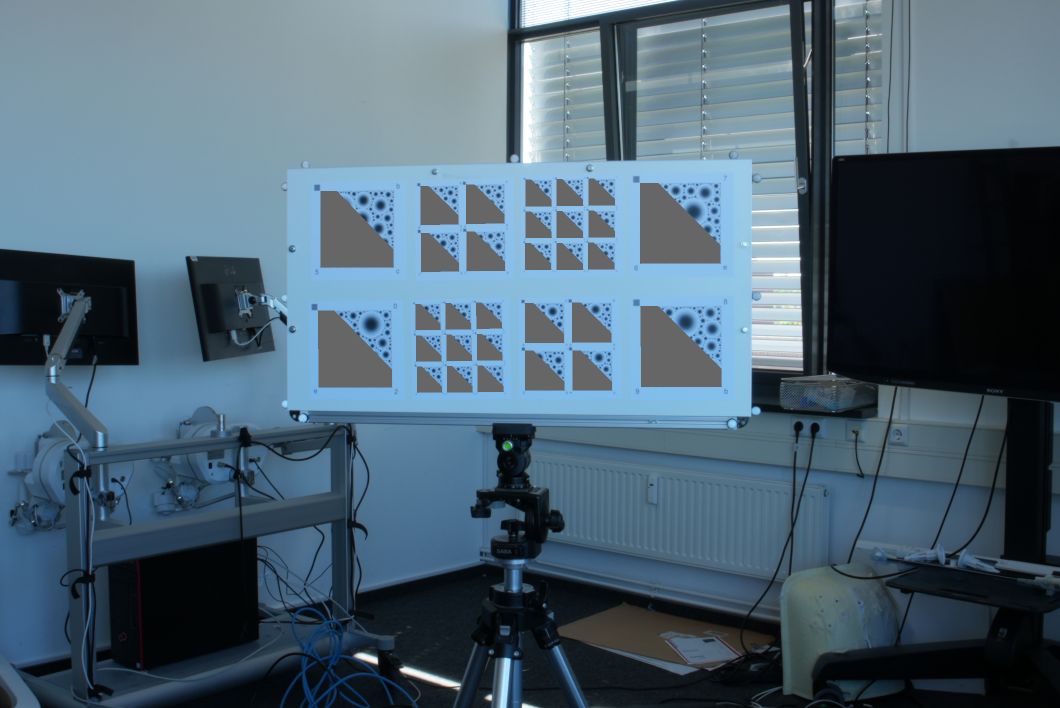
\includegraphics[width=\linewidth]{images/occ_setup/70/compressed_bb_DSC04549.png}
		\end{minipage}\hfill
		\begin{minipage}[c]{0.31\linewidth}
			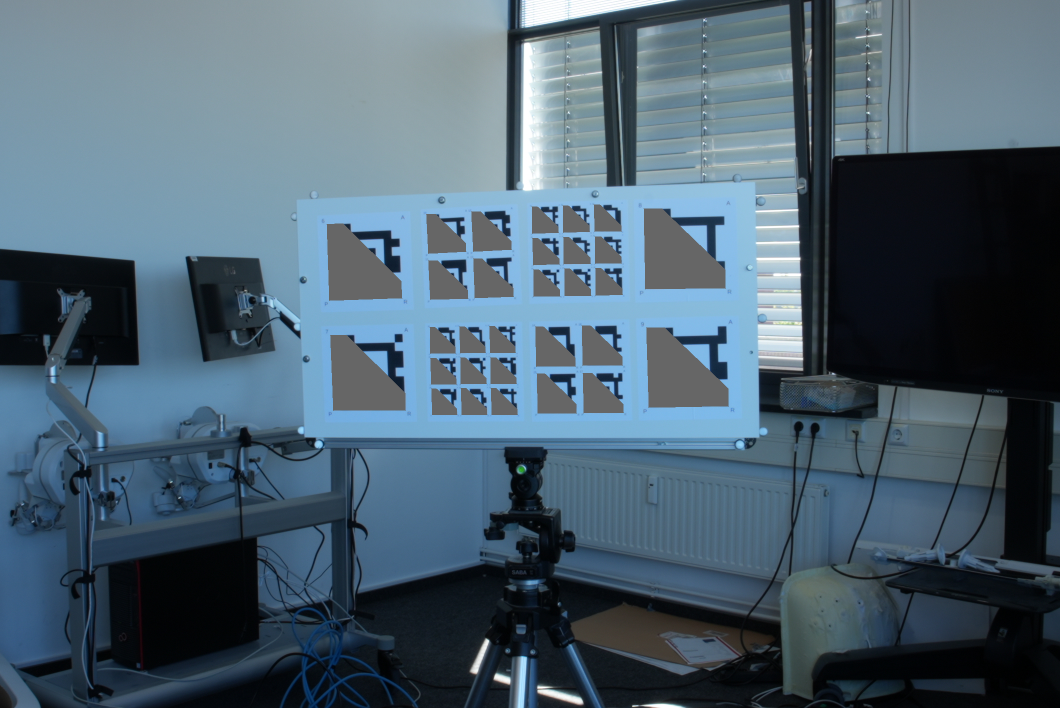
\includegraphics[width=\linewidth]{images/occ_setup/70/compressed_apr_DSC04451.png}
		\end{minipage}\hfill
		\begin{minipage}[c]{0.31\linewidth}
			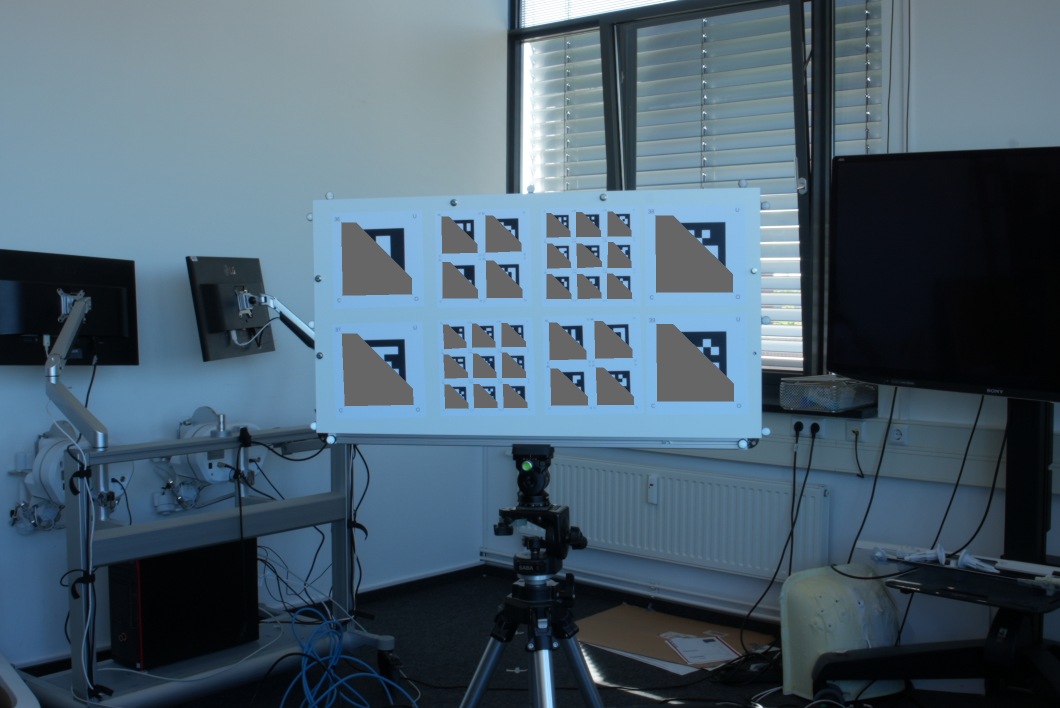
\includegraphics[width=\linewidth]{images/occ_setup/70/compressed_uco_DSC04362.png}
		\end{minipage}
	\end{center}

    \bigskip

    \begin{minipage}{\linewidth}
		\begin{center}
			\figheading{accuracy and probability of detection for occluded boards}
			\resizebox{\linewidth}{!}{%
			\paperfontsettings
			% occlusion_sweep_table.tex — generated by error_distributions.jl; do not edit by hand
\centering
\setlength{\tabcolsep}{2pt}
\providecolor{bbBlue}{HTML}{0072B2}
\providecolor{bbOrange}{HTML}{E69F00}
\providecolor{bbGreen}{HTML}{009E73}
\begin{tabular}{@{}ccc@{}}
% occ_rot.tex — generated (occlusion sweep) by error_distributions.jl; do not edit by hand
\providecolor{bbBlue}{HTML}{0072B2}
\providecolor{bbOrange}{HTML}{E69F00}
\providecolor{bbGreen}{HTML}{009E73}
\begin{tikzpicture}[baseline=(current bounding box.center)]
\begin{axis}[width=4.05cm, height=3.4cm, xmin=-5, xmax=95,
  ylabel={median error ($^\circ$)}, xlabel={occlusion level},
  xtick={0,30,60,90}, xticklabels={{0\%},{30\%},{60\%},{90\%}},
  ymode=log, log ticks with fixed point, ytick={0.5,1,2,5,10,25},
  label style={font=\scriptsize}, tick label style={font=\scriptsize},
  ]
\addplot[draw=bbBlue, line width=1.0pt, mark=*, mark size=1.1pt, mark options={fill=bbBlue, draw=bbBlue}] coordinates {(0,1.124) (10,1.122) (20,1.137) (30,1.112) (40,1.151) (50,1.038) (60,0.872) (70,0.83) (80,0.7412) (90,0.9127)};
\addplot[draw=bbOrange, line width=1.0pt, mark=*, mark size=1.1pt, mark options={fill=bbOrange, draw=bbOrange}] coordinates {(0,1.242) (10,1.617)};
\addplot[draw=bbGreen, line width=1.0pt, mark=*, mark size=1.1pt, mark options={fill=bbGreen, draw=bbGreen}] coordinates {(0,3.036) (10,18.79) (20,24.24)};
\end{axis}
\end{tikzpicture}
 & % occ_trans.tex — generated (occlusion sweep) by error_distributions.jl; do not edit by hand
\providecolor{bbBlue}{HTML}{0072B2}
\providecolor{bbOrange}{HTML}{E69F00}
\providecolor{bbGreen}{HTML}{009E73}
\begin{tikzpicture}[baseline=(current bounding box.center)]
\begin{axis}[width=4.05cm, height=3.4cm, xmin=-5, xmax=95,
  ylabel={median error (mm)}, xlabel={occlusion level},
  xtick={0,30,60,90}, xticklabels={{0\%},{30\%},{60\%},{90\%}},
  ymode=log, log ticks with fixed point, ytick={5,10,25,50,100},
  label style={font=\scriptsize}, tick label style={font=\scriptsize},
  ]
\addplot[draw=bbBlue, line width=1.0pt, mark=*, mark size=1.1pt, mark options={fill=bbBlue, draw=bbBlue}] coordinates {(0,3.777) (10,3.811) (20,3.822) (30,3.937) (40,4.099) (50,3.896) (60,3.882) (70,3.69) (80,3.525) (90,3.49)};
\addplot[draw=bbOrange, line width=1.0pt, mark=*, mark size=1.1pt, mark options={fill=bbOrange, draw=bbOrange}] coordinates {(0,25.62) (10,33.0)};
\addplot[draw=bbGreen, line width=1.0pt, mark=*, mark size=1.1pt, mark options={fill=bbGreen, draw=bbGreen}] coordinates {(0,19.04) (10,91.21) (20,107.6)};
\end{axis}
\end{tikzpicture}
 & % occ_pod.tex — generated (occlusion sweep) by error_distributions.jl; do not edit by hand
\providecolor{bbBlue}{HTML}{0072B2}
\providecolor{bbOrange}{HTML}{E69F00}
\providecolor{bbGreen}{HTML}{009E73}
\begin{tikzpicture}[baseline=(current bounding box.center)]
\begin{axis}[width=4.05cm, height=3.4cm, xmin=-5, xmax=95,
  ylabel={$P(\mathrm{detection})$}, xlabel={occlusion level},
  xtick={0,30,60,90}, xticklabels={{0\%},{30\%},{60\%},{90\%}},
  ymin=0, ymax=1.05, ytick={0,0.25,0.5,0.75,1}, yticklabels={0,,0.5,,1},
  label style={font=\scriptsize}, tick label style={font=\scriptsize},
  ]
\addplot[draw=bbBlue, line width=1.0pt, mark=*, mark size=1.1pt, mark options={fill=bbBlue, draw=bbBlue}] coordinates {(0,0.7982) (10,0.7982) (20,0.7964) (30,0.7893) (40,0.7649) (50,0.6958) (60,0.6125) (70,0.5143) (80,0.3827) (90,0.25)};
\addplot[draw=bbOrange, line width=1.0pt, mark=*, mark size=1.1pt, mark options={fill=bbOrange, draw=bbOrange}] coordinates {(0,0.7281) (10,0.1099) (20,0.0005848) (30,0.0005848) (40,0.0005848) (50,0.0005848) (60,0.0005848) (70,0.0005848) (80,0.0005848) (90,0.0005848)};
\addplot[draw=bbGreen, line width=1.0pt, mark=*, mark size=1.1pt, mark options={fill=bbGreen, draw=bbGreen}] coordinates {(0,0.569) (10,0.2304) (20,0.1023) (30,0.002924) (40,0.004094) (50,0.0) (60,0.0) (70,0.0) (80,0.0) (90,0.0)};
\end{axis}
\end{tikzpicture}
 \\[1pt]
(a) Rotation error & (b) Translation error & (c) Probability of detection \\
\end{tabular}\\[4pt]
\begin{tikzpicture}[baseline]
\draw[bbBlue, line width=1.2pt] (0.0cm,0) -- (0.6cm,0);
\node[anchor=west, font=\small] at (0.7cm,0) {BlobBoards};
\draw[bbOrange, line width=1.2pt] (3.0cm,0) -- (3.6cm,0);
\node[anchor=west, font=\small] at (3.7cm,0) {AprilTag};
\draw[bbGreen, line width=1.2pt] (6.0cm,0) -- (6.6cm,0);
\node[anchor=west, font=\small] at (6.7cm,0) {ArUco};
\end{tikzpicture}

			}
		\end{center}
	\end{minipage}
}

\block{Conclusion}{
	{\textbf{state of the art marker} in pose accuracy and occlusion robustness}

	\bigskip

\begin{center}

	\begin{minipage}[c]{0.19\linewidth}
		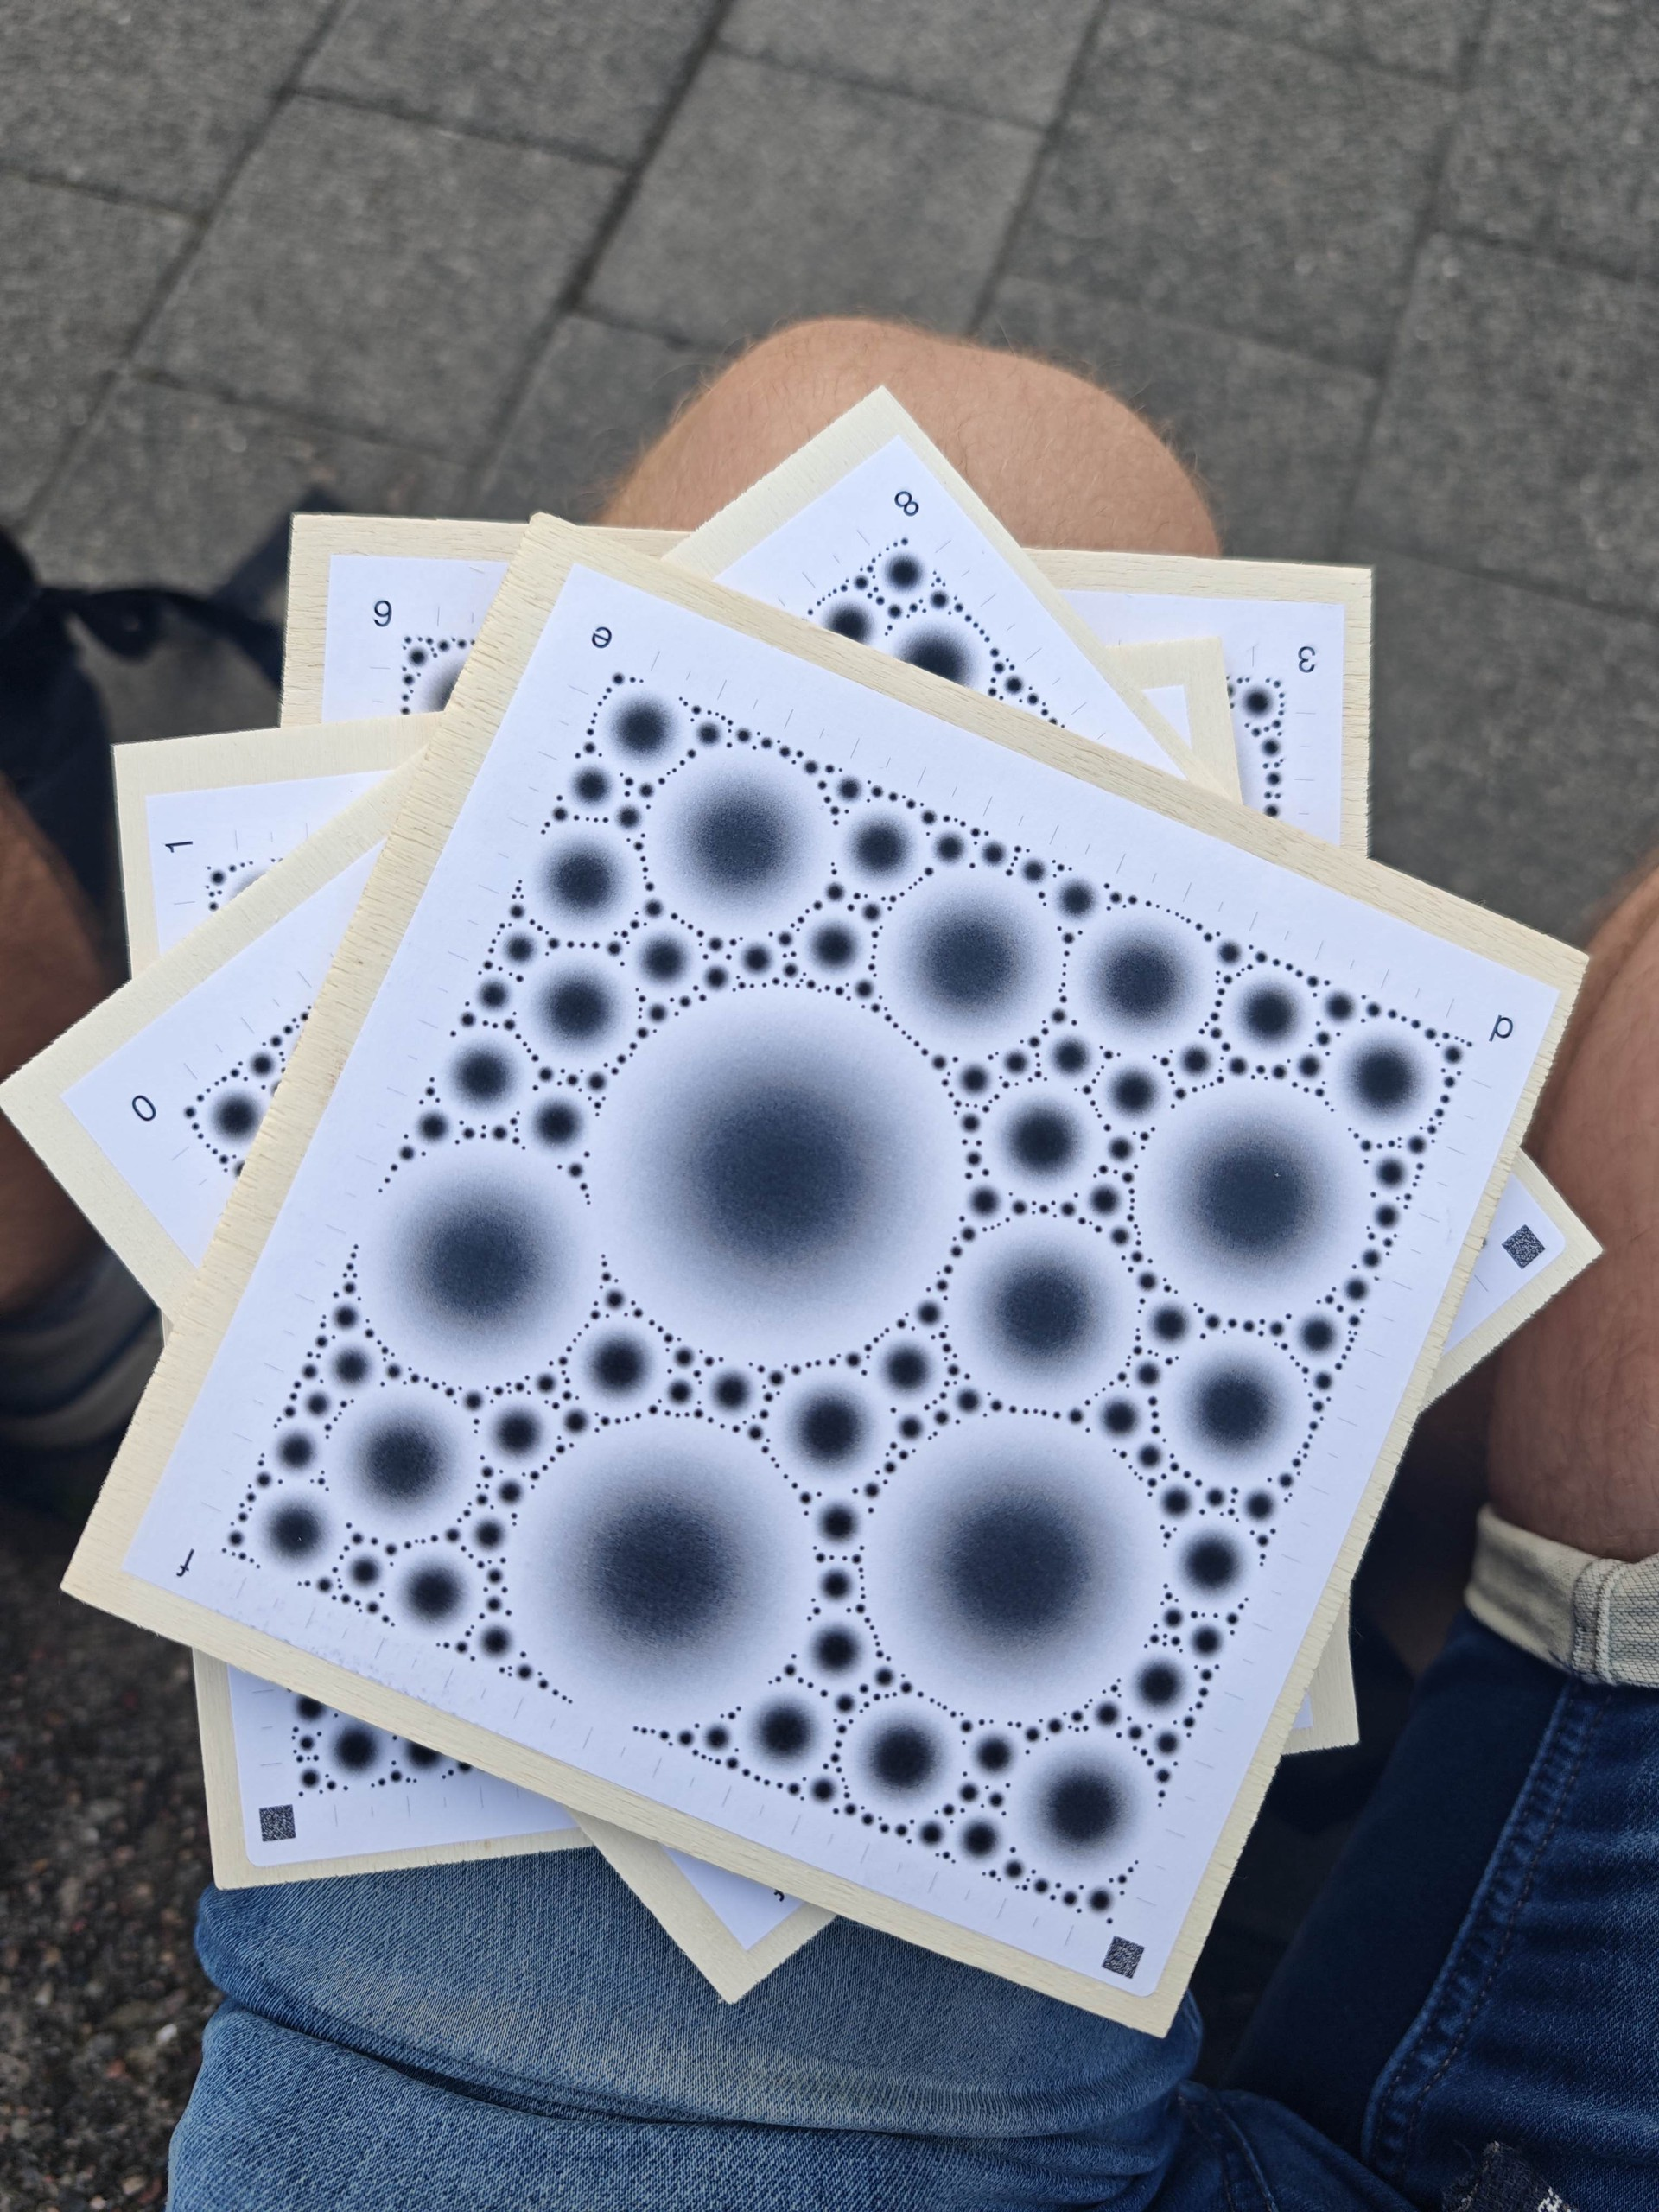
\includegraphics[width=\linewidth]{images/adapted/original.jpg}
	\end{minipage}\hfill
	\begin{minipage}[c]{0.19\linewidth}
		\overlaid[width=\linewidth]{images/adapted/original.jpg}{images/adapted/adapted_fde.pdf}
	\end{minipage}\hfill
	\begin{minipage}[c]{0.19\linewidth}
		\overlaid[width=\linewidth]{images/adapted/original.jpg}{images/adapted/adapted_f80.pdf}
	\end{minipage}\hfill
	\begin{minipage}[c]{0.19\linewidth}
		\overlaid[width=\linewidth]{images/adapted/original.jpg}{images/adapted/adapted_336.pdf}
	\end{minipage}\hfill
	\begin{minipage}[c]{0.19\linewidth}
		\overlaid[width=\linewidth]{images/adapted/original.jpg}{images/adapted/adapted_14b.pdf}
	\end{minipage}
\end{center}
\bigskip
\begin{center}
	\figheading{future work}
	\begin{minipage}[t]{0.48\linewidth}
		\centering
		{camera calibration}\\[\subcaptiongap]
		% \overlaid[width=\linewidth]{images/fisheye_overlays_photo.jpg}{images/fisheye_overlays.pdf}
		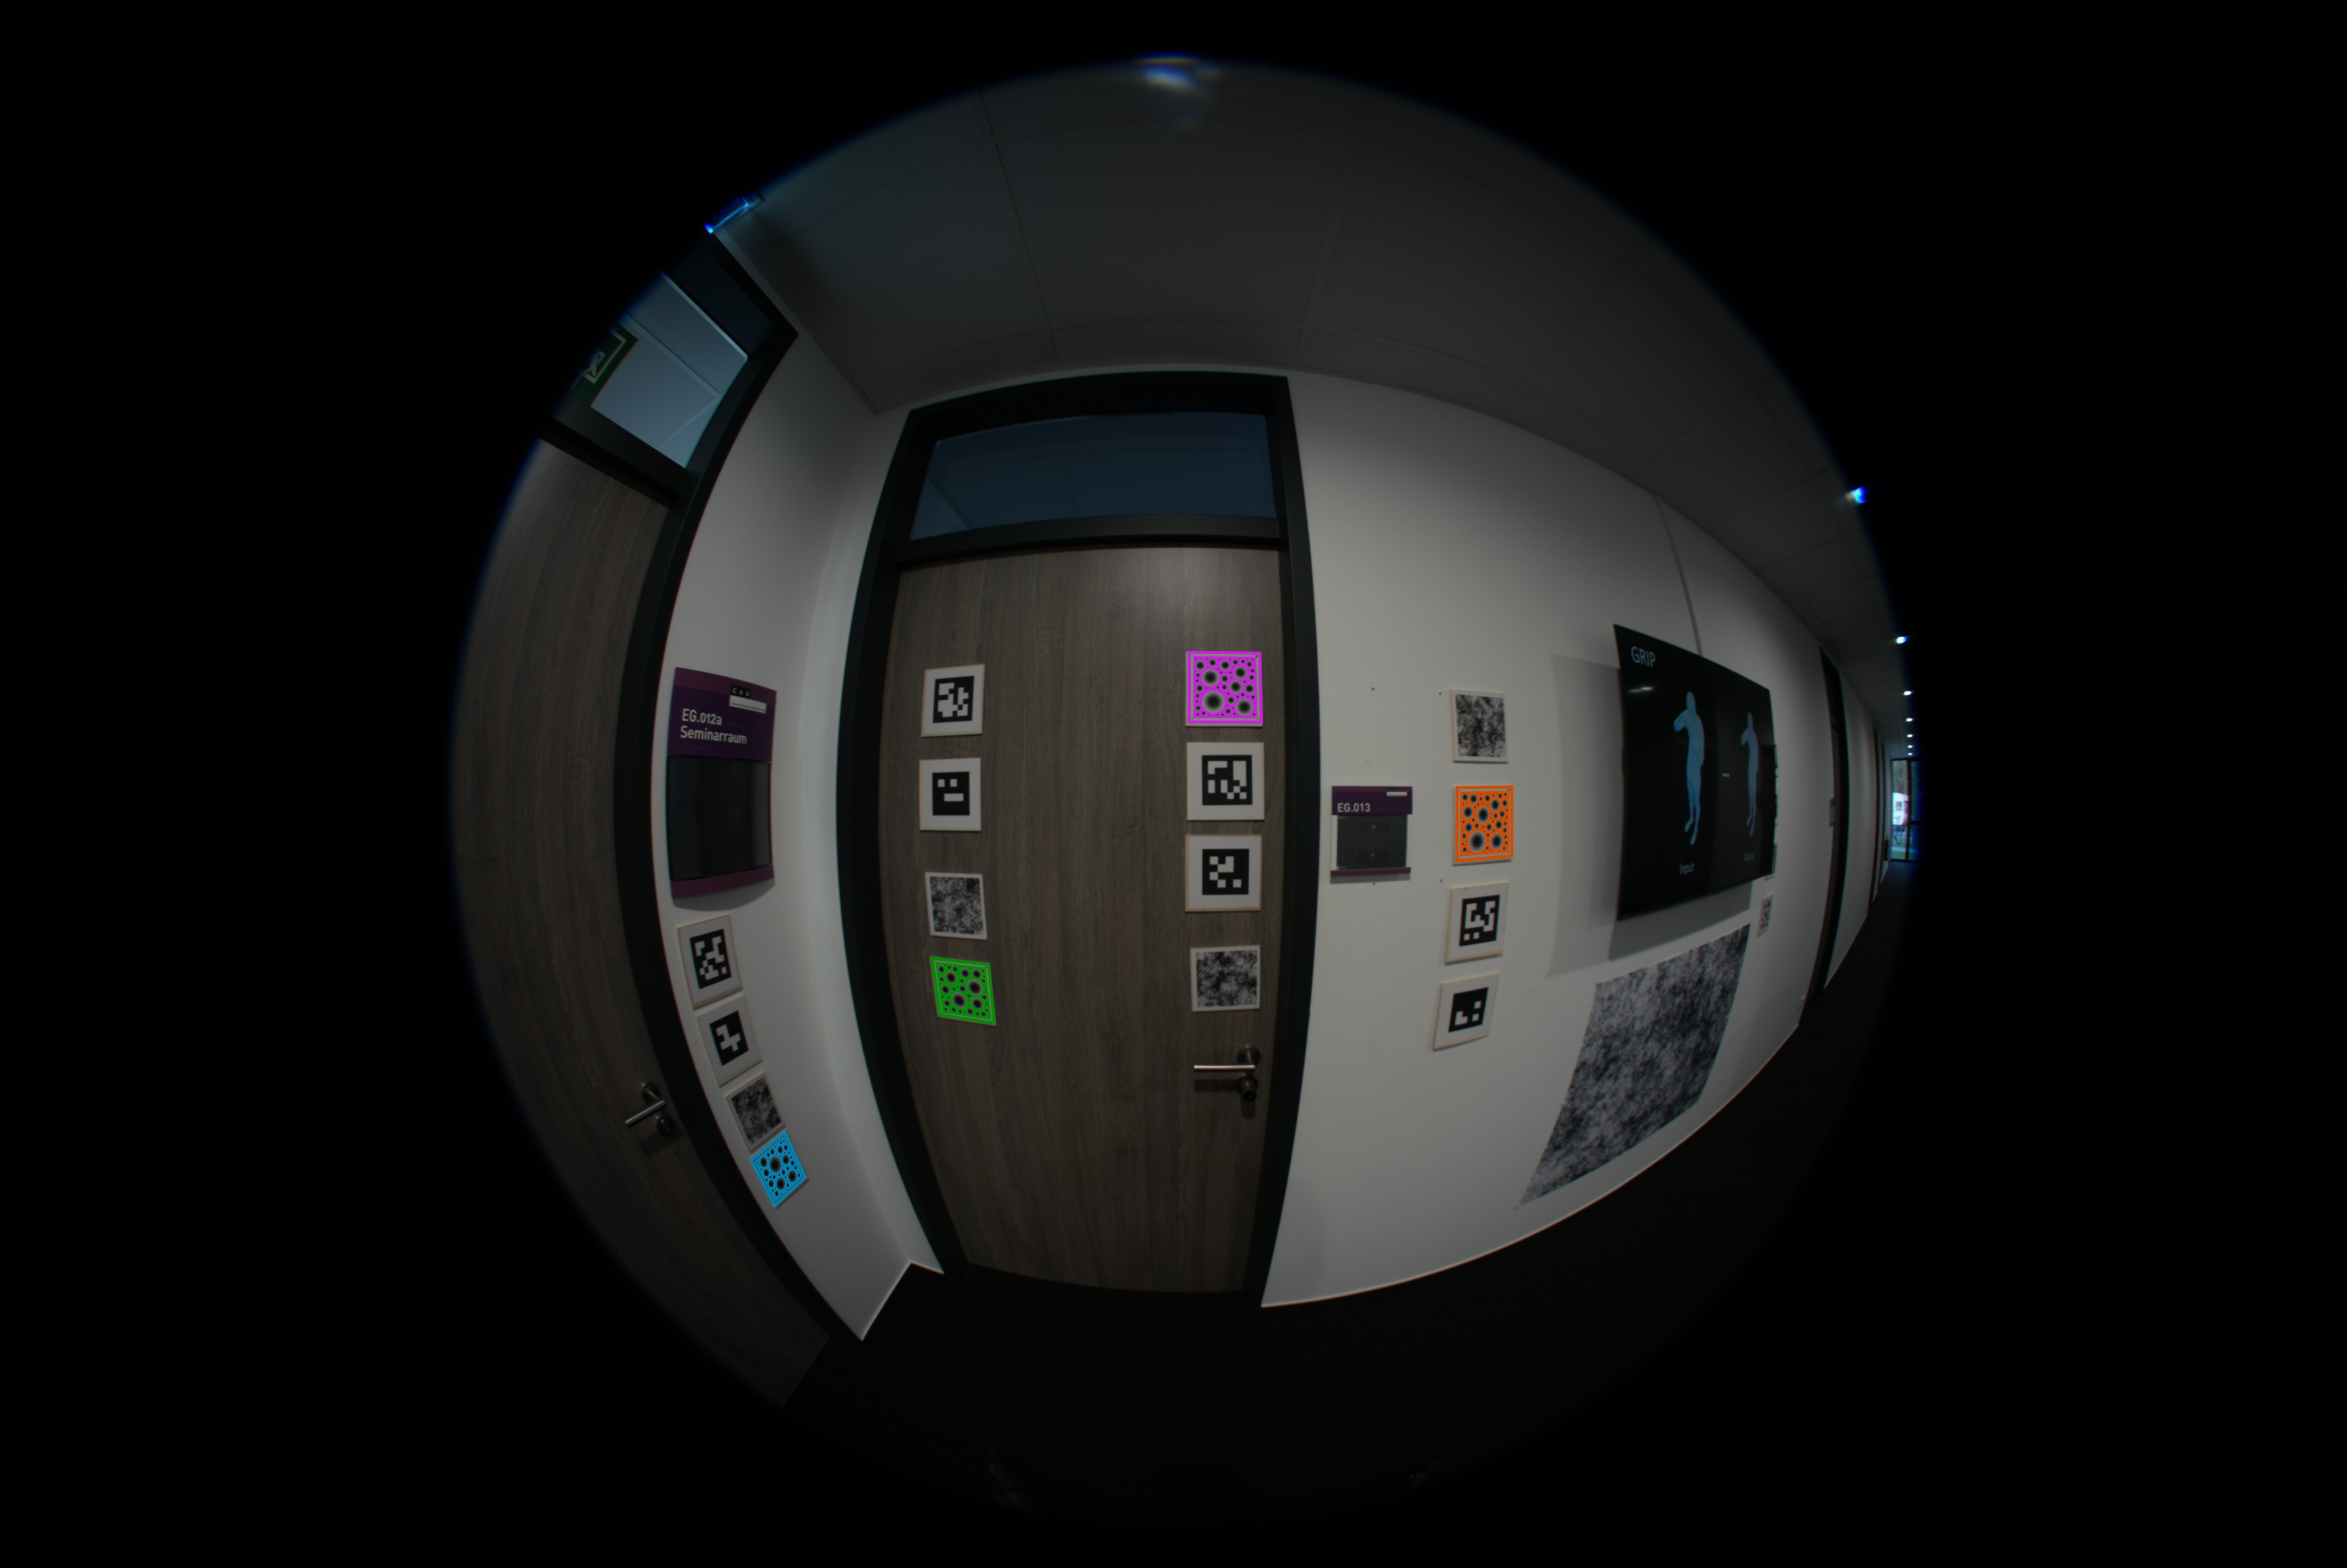
\includegraphics[width=\linewidth]{images/fisheye_overlays.jpg}
	\end{minipage}%
	\hfill%
	\begin{minipage}[t]{0.48\linewidth}
		\centering
		{real time application}\\[\subcaptiongap]
		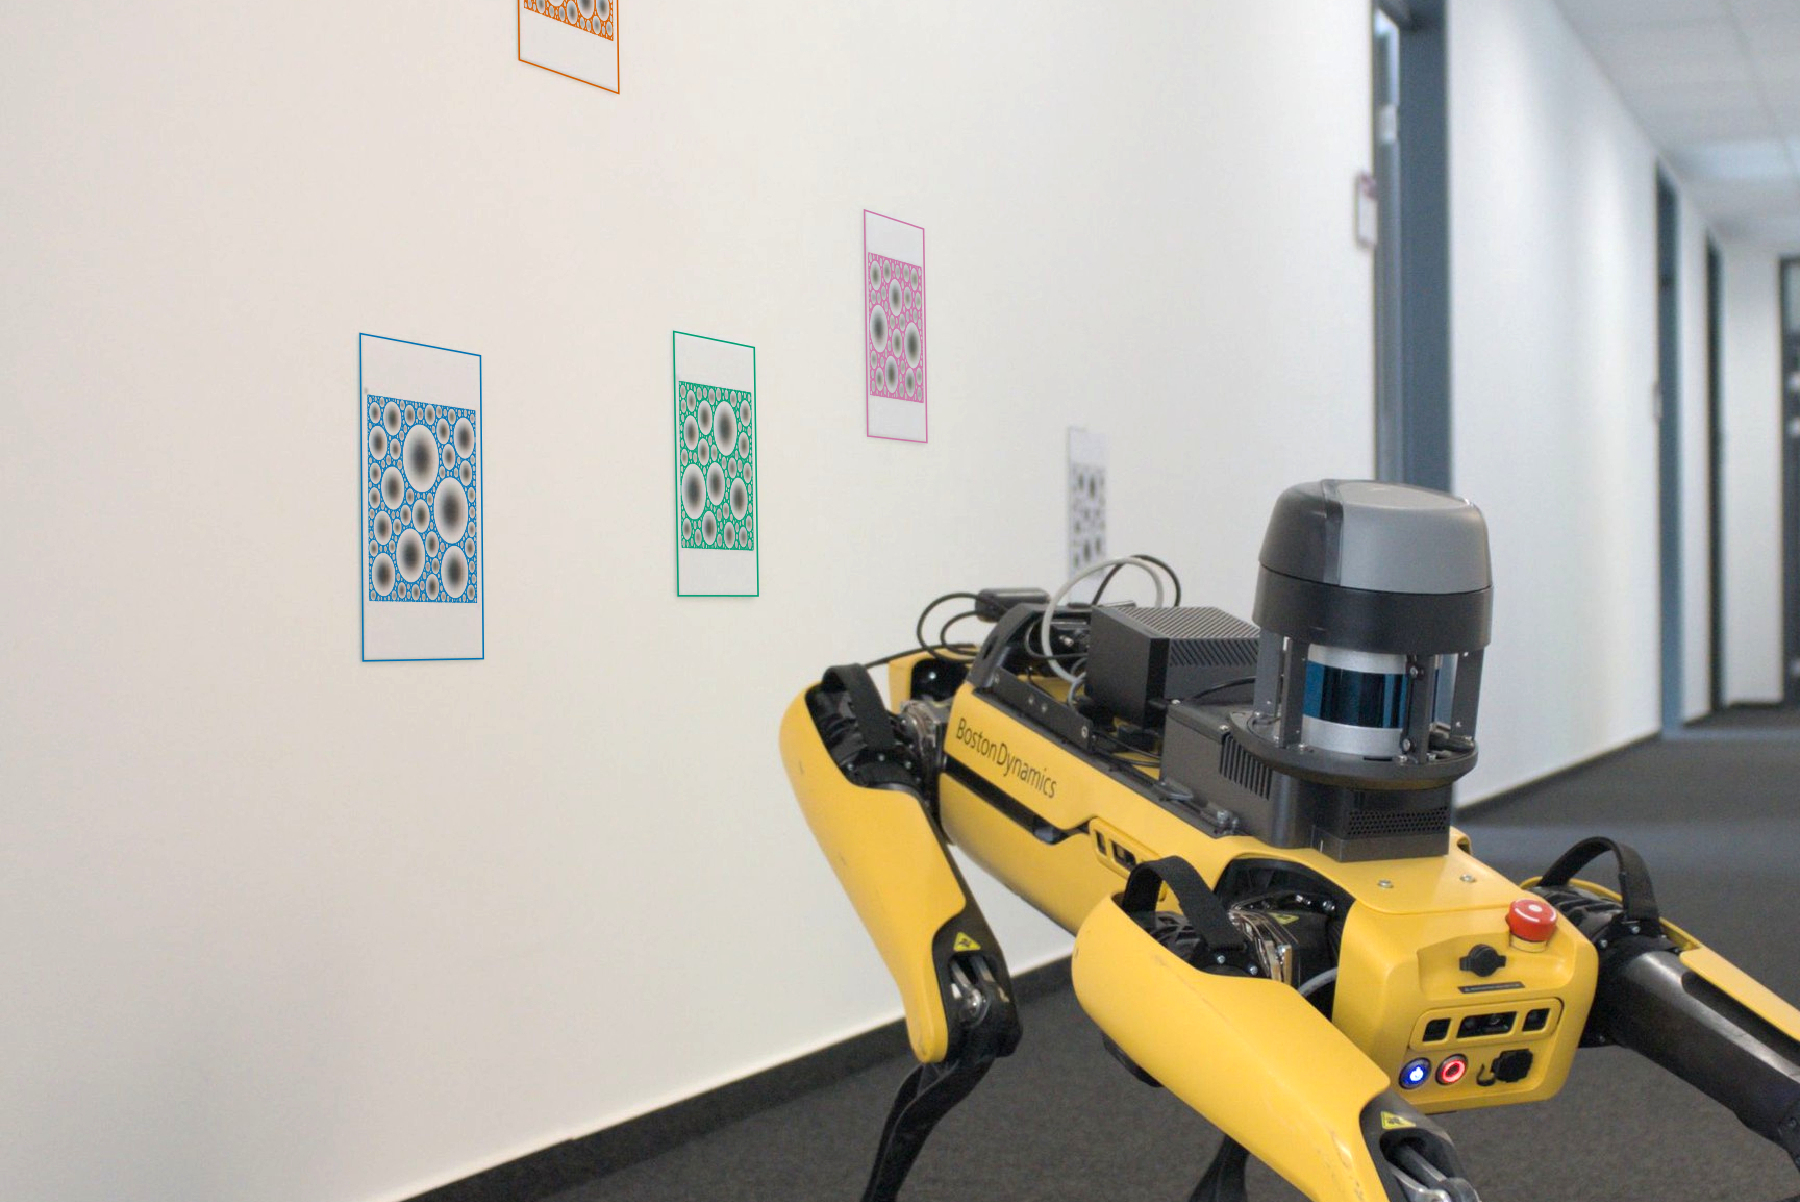
\includegraphics[width=\linewidth]{images/robot.jpg}
	\end{minipage}
\end{center}
}

\end{columns}

\end{document}
